\documentclass[12pt]{article}

% Paquetes necesarios
\usepackage{graphicx}
\usepackage{geometry}
\usepackage[utf8]{inputenc}
\usepackage[spanish]{babel}
\usepackage{booktabs}
\usepackage{tabularx}
\usepackage{multirow}
\usepackage{caption}
\usepackage{array}
\usepackage{pdflscape}
\usepackage{amsmath}
\usepackage{amssymb}
\usepackage{bm}
\usepackage{amsfonts}
\usepackage{enumitem}
\usepackage{longtable}
\usepackage{rotating}
\usepackage{afterpage}
\usepackage{xcolor}
\usepackage{listings}
\usepackage{float}
\usepackage{pdfpages}
\usepackage[colorlinks=true, linkcolor=blue!70!black, citecolor=blue!70!black, urlcolor=blue!70!black]{hyperref}

% Configuración profesional de listings para C++ y Python
\definecolor{codegreen}{rgb}{0.1,0.6,0.2}
\definecolor{codegray}{rgb}{0.5,0.5,0.5}
\definecolor{codepurple}{rgb}{0.58,0,0.82}
\definecolor{backcolour}{rgb}{0.97,0.97,0.97}

\lstdefinestyle{codestyle}{
    backgroundcolor=\color{backcolour},   
    commentstyle=\color{codegreen}\itshape,
    keywordstyle=\color{blue}\bfseries,
    numberstyle=\tiny\color{codegray},
    stringstyle=\color{codepurple},
    basicstyle=\ttfamily\footnotesize,
    breakatwhitespace=false,         
    breaklines=true,                 
    captionpos=b,                    
    keepspaces=true,                 
    numbers=left,                    
    numbersep=5pt,                  
    showspaces=false,                
    showstringspaces=false,
    showtabs=false,                  
    tabsize=2,
    frame=single,
    rulecolor=\color{codegray!30}
}
\lstset{style=codestyle}

\geometry{left=3cm, right=3cm, top=2.5cm, bottom=2.5cm}

\begin{document}

% =========================================================================
% PORTADA OFICIAL INSTITUCIONAL UPIITA - IPN (UpiiTeXis)
% =========================================================================
% Incorpora la carátula oficial reglamentaria con franja lateral, heráldica
% institucional (IPN / UPIITA) y líneas formales de firmas para:
%   - Alumno: Ramiro Mendoza Diaz
%   - Asesor: Dr. Jorge Alejandro Juárez Lora
%   - Presidente del Jurado: Dra. Blanca Rosa Briseño Tepepa
%   - Profesor titular: M. en C. Cecilia Fernández Nava
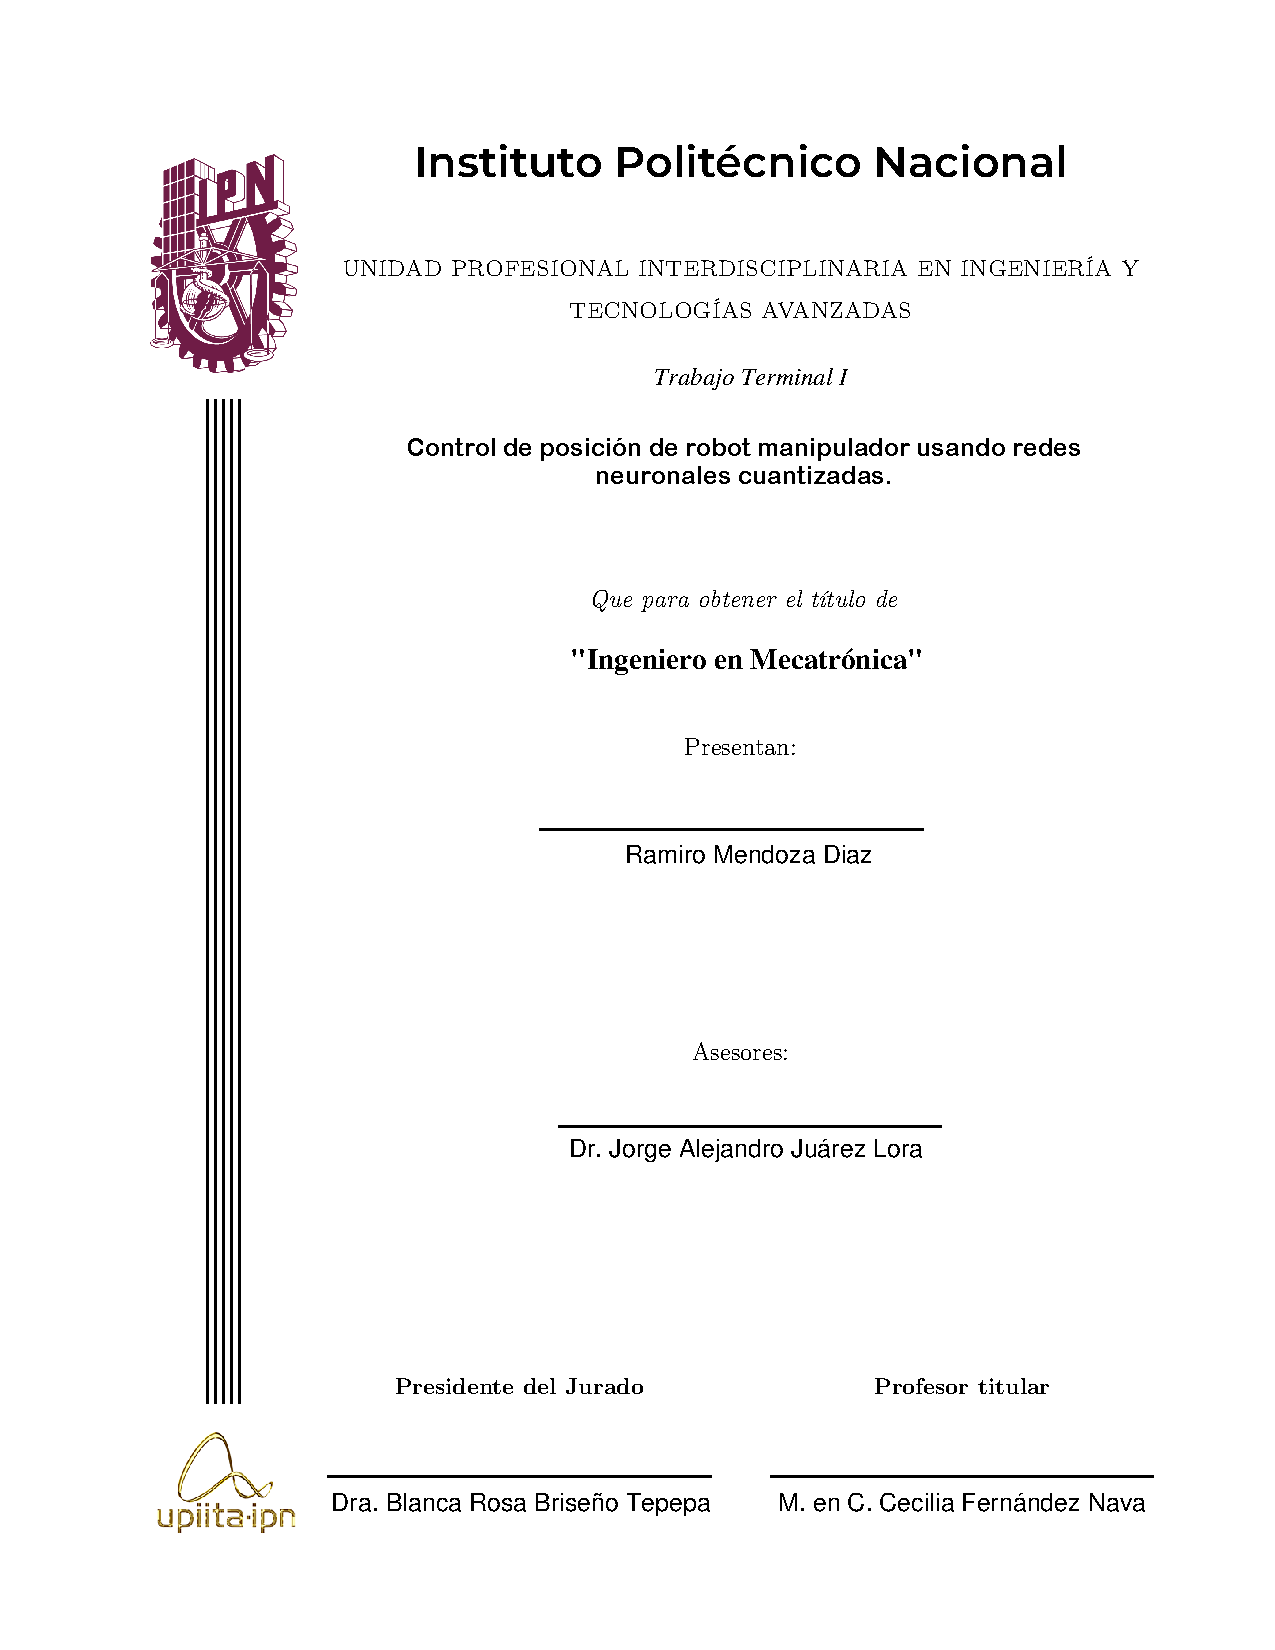
\includepdf[pages=1]{portada_upiita.pdf}

\pagenumbering{roman}
\setcounter{page}{2}

\newpage
\tableofcontents

\newpage
\addcontentsline{toc}{section}{Resumen}
{\large \textbf{Resumen}}\\
El despliegue de controladores avanzados basados en Redes Neuronales Profundas (DNNs) en la robótica de manipulación enfrenta restricciones severas de latencia y consumo energético impuestas por el cuello de botella de Von Neumann y la barrera de memoria en sistemas de cómputo embebidos. En lazos de control cerrados en tiempo real ($100\text{ Hz} - 500\text{ Hz}$), la evaluación continua de modelos densos en punto flotante (FP32) degrada la predictibilidad temporal e incrementa la potencia disipada. En este contexto, el presente reporte de Trabajo Terminal 1 aborda el diseño, implementación y verificación de un esquema mecatrónico híbrido de control de posición para un robot manipulador serial de 6 grados de libertad (Universal Robots UR3e), integrando dinámica analítica inversa con una Red Neuronal Cuantizada a enteros de 8 bits (QNN-INT8).

La metodología implementada articula una ley de control por par calculado (\textit{Computed Torque Control}) donde el Algoritmo Recursivo de Newton-Euler (RNEA), programado en C++17 evitando la realización de asignaciones dinámicas en su evaluación recursiva, compensa las no linealidades mecánicas nominales ($\mathcal{O}(n)$). De forma complementaria, una red neuronal perceptrón multicapa (MLP) con vector de características de 42 dimensiones estima en línea las dinámicas residuales no modeladas y fricciones articulares. El modelo fue entrenado en PyTorch, exportado al estándar ONNX y cuantizado mediante Cuantización Dinámica Post-Entrenamiento (\textit{Dynamic PTQ}) a INT8, ejecutándose dentro del middleware ROS 2 Jazzy Jalisco con el motor ONNX Runtime monohilo en C++. La verificación experimental se llevó a cabo en un gemelo digital de alta fidelidad (\textit{Sim-to-Real}) desarrollado en Gazebo Harmonic gobernado por la arquitectura modular de \texttt{ros2\_control} a una frecuencia de $500\text{ Hz}$ ($T_s = 2\text{ ms}$).

Los resultados empíricos demuestran que la cuantización a INT8 redujo la huella de memoria del modelo en un $74.43\%$ (de $1.23\text{ MB}$ a $315\text{ KB}$) y aceleró la latencia media de inferencia a $29.2\,\mu\text{s}$. El tiempo de cómputo medio por ciclo de control fue de $215.4\,\mu\text{s}$ (con un máximo observado de $299.7\,\mu\text{s}$ en la muestra experimental), proporcionando una holgura temporal empírica del $89.23\%$ frente al periodo de muestreo admisible ($T_s = 2000\,\mu\text{s}$) y acotando los pares de esfuerzo estrictamente dentro de los límites mecánicos ($\pm 55.0\text{ N}\cdot\text{m}$). Si bien el lazo cerrado continuo acumula un incremento en el error cuadrático medio articular ($\text{RMSE} = 0.138\text{ rad}$) respecto al modelo en punto flotante ($0.092\text{ rad}$) debido a la discretización afín y a la asignación de $\ddot{\bm{q}}_{act} = \bm{0}$ para evitar ruido de diferenciación numérica, el seguimiento articular permaneció dentro de la envolvente funcional definida para las pruebas de simulación. Estos hallazgos validan la viabilidad algorítmica y la reducción del costo computacional de la arquitectura, sentando la base técnica para el entrenamiento consciente de cuantización (QAT), la instrumentación y medición física de potencia eléctrica y la aceleración en hardware neutro (FPGA / SoC Zynq) en Trabajo Terminal 2.

\vspace{0.6cm}
\textbf{Palabras clave:} Redes Neuronales Cuantizadas, Robótica de Manipulación, Control por Par Calculado, Cuantización Dinámica, ROS 2, INT8, Sim-to-Real.

\vspace{1.0cm}
\addcontentsline{toc}{section}{Abstract}
{\large \textbf{Abstract}}\\
The deployment of advanced controllers based on Deep Neural Networks (DNNs) in robotic manipulation faces severe latency and energy constraints imposed by the Von Neumann bottleneck and the memory wall in embedded computing platforms. In closed real-time control loops ($100\text{ Hz} - 500\text{ Hz}$), continuous evaluation of high-density floating-point models (FP32) degrades temporal predictability and escalates power dissipation. In this context, this Term Project 1 report presents the design, implementation, and verification of a hybrid mechatronic position control scheme for a 6-DOF serial manipulator (Universal Robots UR3e), coupling analytical inverse dynamics with an 8-bit integer Quantized Neural Network (QNN-INT8).

The methodology integrates a Computed Torque Control (CTC) framework wherein the Recursive Newton-Euler Algorithm (RNEA), implemented in C++17 avoiding dynamic memory allocations in its recursive evaluation, compensates for nominal mechanical non-linearities with optimal linear complexity ($\mathcal{O}(n)$). Concurrently, a multilayer perceptron (MLP) neural network fed by a 42-dimensional input feature vector estimates unmodeled residual dynamics and joint friction online. The network was trained in PyTorch, exported to the ONNX standard, and compressed via dynamic Post-Training Quantization (Dynamic PTQ) to INT8, running within the ROS 2 Jazzy Jalisco middleware via the single-threaded C++ ONNX Runtime engine. Experimental verification was conducted on a high-fidelity Sim-to-Real digital twin in Gazebo Harmonic managed by the \texttt{ros2\_control} framework at a closed-loop frequency of $500\text{ Hz}$ ($T_s = 2\text{ ms}$).

Empirical results demonstrate that INT8 quantization reduced the model memory footprint by $74.43\%$ (from $1.23\text{ MB}$ down to $315\text{ KB}$) and accelerated mean inference latency to $29.2\,\mu\text{s}$. Total critical-loop execution time averaged $215.4\,\mu\text{s}$ (with an observed empirical maximum of $299.7\,\mu\text{s}$), providing an empirical $89.23\%$ timing margin with respect to the sampling period ($T_s = 2000\,\mu\text{s}$), with commanded torques strictly bounded within physical thresholds ($\pm 55.0\text{ N}\cdot\text{m}$). While closed-loop control exhibits a tracking degradation ($\text{RMSE} = 0.138\text{ rad}$) compared to the floating-point baseline ($0.092\text{ rad}$) due to integer quantization noise and setting $\ddot{\bm{q}}_{act} = \bm{0}$ to prevent numerical differentiation noise, joint trajectory tracking remained strictly within the functional operational envelope defined for the simulation trials. These outcomes validate the algorithmic feasibility and computational overhead reduction of the architecture, establishing the technical foundation for Quantization-Aware Training (QAT), physical electrical power measurement, and embedded hardware acceleration on FPGA / SoC Zynq in Term Project 2.

\vspace{0.6cm}
\textbf{Keywords:} Quantized Neural Networks, Robotic Manipulation, Computed Torque Control, Dynamic Quantization, ROS 2, INT8, Sim-to-Real.

\newpage
\addcontentsline{toc}{section}{Índice de figuras}
\listoffigures

\newpage
\addcontentsline{toc}{section}{Índice de tablas}
\listoftables

\newpage
\section*{Nomenclatura}
\addcontentsline{toc}{section}{Nomenclatura}

En la Tabla \ref{tab:nomenclatura} se presentan los acrónimos, términos técnicos y abreviaturas especializadas utilizadas a lo largo de este documento, ordenadas alfabéticamente.

\vspace{0.5cm}
\begin{longtable}{p{0.22\linewidth} p{0.72\linewidth}}
\caption{Acrónimos y términos técnicos empleados en el proyecto.} \label{tab:nomenclatura} \\
\toprule
\textbf{Término / Sigla} & \textbf{Significado y Descripción Técnica} \\
\midrule
\endfirsthead
\toprule
\textbf{Término / Sigla} & \textbf{Significado y Descripción Técnica} \\
\midrule
\endhead
\midrule
\multicolumn{2}{r}{\textit{Continúa en la siguiente página...}} \\
\bottomrule
\endfoot
\bottomrule
\endlastfoot
\textbf{AI / IA} & Inteligencia Artificial (\textit{Artificial Intelligence}). \\
\textbf{ANN} & Red Neuronal Artificial (\textit{Artificial Neural Network}). \\
\textbf{CIM} & Computación en Memoria (\textit{Computing-In-Memory}). \\
\textbf{CoM} & Centro de Masa (\textit{Center of Mass}) de un eslabón rígido. \\
\textbf{CTC} & Control por Par Computado (\textit{Computed Torque Control}). \\
\textbf{DH} & Denavit-Hartenberg (convención cinemática modificada de parámetros geométricos). \\
\textbf{DNN} & Red Neuronal Profunda (\textit{Deep Neural Network}). \\
\textbf{FP32} & Formato de punto flotante de precisión simple de 32 bits (estándar IEEE 754). \\
\textbf{FPGA} & Matriz de Puertas Lógicas Programable en Campo (\textit{Field-Programmable Gate Array}). \\
\textbf{GDL} & Grados de Libertad (\textit{Degrees of Freedom}, DoF). \\
\textbf{INT8} & Formato numérico entero con signo de 8 bits (rango $[-128, 127]$). \\
\textbf{MAC} & Operación de Multiplicación y Acumulación (\textit{Multiply-Accumulate}). \\
\textbf{MAE} & Error Absoluto Medio (\textit{Mean Absolute Error}). \\
\textbf{MCAP} & Formato de almacenamiento eficiente para grabación de datos y telemetría en ROS 2. \\
\textbf{ML} & Aprendizaje Automático (\textit{Machine Learning}). \\
\textbf{MLP} & Perceptrón Multicapa (\textit{Multilayer Perceptron}). \\
\textbf{MSE} & Error Cuadrático Medio (\textit{Mean Squared Error}). \\
\textbf{ONNX} & Formato Abierto para Intercambio de Redes Neuronales (\textit{Open Neural Network Exchange}). \\
\textbf{PD / PID} & Controlador Proporcional-Derivativo / Proporcional-Integral-Derivativo. \\
\textbf{PINN} & Red Neuronal Informada por la Física (\textit{Physics-Informed Neural Network}). \\
\textbf{PTQ} & Cuantización Post-Entrenamiento (\textit{Post-Training Quantization}). \\
\textbf{QAT} & Entrenamiento Consciente de Cuantización (\textit{Quantization-Aware Training}). \\
\textbf{QNN} & Red Neuronal Cuantizada (\textit{Quantized Neural Network}). \\
\textbf{QoS} & Calidad de Servicio (\textit{Quality of Service}) en protocolos de transporte ROS 2. \\
\textbf{RNEA} & Algoritmo Recursivo de Newton-Euler (\textit{Recursive Newton-Euler Algorithm}). \\
\textbf{RMSE} & Raíz del Error Cuadrático Medio (\textit{Root Mean Square Error}). \\
\textbf{ROS / ROS 2} & Sistema Operativo de Robots (\textit{Robot Operating System} versión 2). \\
\textbf{RT} & Tiempo Real (\textit{Real-Time}). \\
\textbf{SNN} & Red Neuronal de Impulsos (\textit{Spiking Neural Network}). \\
\textbf{UR3e} & Robot manipulador colaborativo industrial de 6 GDL de Universal Robots. \\
\textbf{URDF} & Formato Unificado de Descripción de Robots (\textit{Unified Robot Description Format}). \\
\textbf{VoBo} & Visto Bueno de aprobación emitido por el jurado o asesores. \\
\end{longtable}

\newpage
\section*{Simbología}
\addcontentsline{toc}{section}{Simbología}

En la Tabla \ref{tab:simbologia} se detallan las variables matemáticas, operadores, vectores y matrices empleados en la formulación cinemática, dinámica y de control, especificando sus unidades en el Sistema Internacional (SI).

\vspace{0.5cm}
\begin{longtable}{p{0.20\linewidth} p{0.62\linewidth} p{0.14\linewidth}}
\caption{Simbología matemática y magnitudes físicas del sistema mecatrónico.} \label{tab:simbologia} \\
\toprule
\textbf{Símbolo} & \textbf{Descripción Física o Matemática} & \textbf{Unidad (SI)} \\
\midrule
\endfirsthead
\toprule
\textbf{Símbolo} & \textbf{Descripción Física o Matemática} & \textbf{Unidad (SI)} \\
\midrule
\endhead
\midrule
\multicolumn{3}{r}{\textit{Continúa en la siguiente página...}} \\
\bottomrule
\endfoot
\bottomrule
\endlastfoot
\multicolumn{3}{l}{\textit{\textbf{Cinemática y Variables Articulares:}}} \\
$\bm{q} = [q_1, \dots, q_6]^T$ & Vector de posiciones articulares generalizadas & $\text{rad}$ \\
$\dot{\bm{q}} = [\dot{q}_1, \dots, \dot{q}_6]^T$ & Vector de velocidades articulares & $\text{rad/s}$ \\
$\ddot{\bm{q}} = [\ddot{q}_1, \dots, \ddot{q}_6]^T$ & Vector de aceleraciones articulares & $\text{rad/s}^2$ \\
$\bm{q}_d, \dot{\bm{q}}_d, \ddot{\bm{q}}_d$ & Trayectorias articular deseada (posición, velocidad y aceleración) & $\text{rad}, \text{rad/s}, \text{rad/s}^2$ \\
$\bm{e} = \bm{q}_d - \bm{q}$ & Vector de error de seguimiento de posición articular & $\text{rad}$ \\
$\dot{\bm{e}} = \dot{\bm{q}}_d - \dot{\bm{q}}$ & Vector de error de velocidad articular & $\text{rad/s}$ \\
$\alpha_{i-1}$ & Parámetro DH modificado: ángulo de torsión de eslabón & $\text{rad}$ \\
$a_{i-1}$ & Parámetro DH modificado: longitud de eslabón & $\text{m}$ \\
$d_i$ & Parámetro DH modificado: desplazamiento en el eje articular & $\text{m}$ \\
$\theta_i$ & Parámetro DH modificado: variable angular articular & $\text{rad}$ \\
$\bm{R}_i^{i-1}$ & Matriz de rotación del marco coordenado $i$ respecto al marco $i-1$ & Adimensional \\
$\bm{P}_i^{i-1}$ & Vector de traslación del origen $i-1$ al origen $i$ expresado en el marco $i$ & $\text{m}$ \\
$\bm{z}_0$ & Vector unitario sobre el eje de rotación articular $[0, 0, 1]^T$ & Adimensional \\
\midrule
\multicolumn{3}{l}{\textit{\textbf{Cinemática Diferencial y Dinámica RNEA (Paso hacia Adelante):}}} \\
$\bm{\omega}_i$ & Vector de velocidad angular del eslabón $i$ expresado en su propio marco & $\text{rad/s}$ \\
$\dot{\bm{\omega}}_i$ & Vector de aceleración angular del eslabón $i$ & $\text{rad/s}^2$ \\
$\dot{\bm{v}}_i$ & Vector de aceleración lineal del origen del marco coordenado $i$ & $\text{m/s}^2$ \\
$\dot{\bm{v}}_{c,i}$ & Vector de aceleración lineal del centro de masa del eslabón $i$ & $\text{m/s}^2$ \\
$\bm{r}_{c,i}$ & Vector de posición local del centro de masa del eslabón $i$ & $\text{m}$ \\
$\bm{g} = [0, 0, 9.81]^T$ & Vector de aceleración de la gravedad terrestre & $\text{m/s}^2$ \\
\midrule
\multicolumn{3}{l}{\textit{\textbf{Dinámica Analítica y Esfuerzos RNEA (Paso hacia Atrás):}}} \\
$m_i$ & Masa total del eslabón $i$ & $\text{kg}$ \\
$\bm{I}_i$ & Tensor de inercia baricéntrico del eslabón $i$ expresado en su marco local & $\text{kg}\cdot\text{m}^2$ \\
$\bm{F}_i$ & Fuerza inercial total que actúa sobre el eslabón $i$ & $\text{N}$ \\
$\bm{N}_i$ & Momento inercial total que actúa sobre el eslabón $i$ & $\text{N}\cdot\text{m}$ \\
$\bm{f}_i$ & Fuerza ejercida por el eslabón $i-1$ sobre el eslabón $i$ & $\text{N}$ \\
$\bm{n}_i$ & Par/momento ejercido por el eslabón $i-1$ sobre el eslabón $i$ & $\text{N}\cdot\text{m}$ \\
$\bm{\tau} = [\tau_1, \dots, \tau_6]^T$ & Vector de pares motores netos generalizados aplicados a las articulaciones & $\text{N}\cdot\text{m}$ \\
$\bm{\tau}_{rnea}$ & Par dinámico de prealimentación calculado por RNEA & $\text{N}\cdot\text{m}$ \\
$\bm{\tau}_{cmd}$ & Par de comando total enviado a las interfaces de esfuerzo de los motores & $\text{N}\cdot\text{m}$ \\
$\bm{M}(\bm{q})$ & Matriz de masa e inercia del manipulador ($6 \times 6$) & $\text{kg}\cdot\text{m}^2$ \\
$\bm{C}(\bm{q},\dot{\bm{q}})$ & Matriz de términos centrífugos y de Coriolis ($6 \times 6$) & $\text{N}\cdot\text{m}\cdot\text{s/rad}$ \\
$\bm{g}(\bm{q})$ & Vector de pares gravitacionales articulares ($6 \times 1$) & $\text{N}\cdot\text{m}$ \\
\midrule
\multicolumn{3}{l}{\textit{\textbf{Control Automático y Parámetros de Redes Neuronales:}}} \\
$\bm{K}_p, \bm{K}_d, \bm{K}_i$ & Matrices de ganancias de retroalimentación proporcional, derivativa e integral & $\text{N}\cdot\text{m/rad}, \text{N}\cdot\text{m}\cdot\text{s/rad}, \text{N}\cdot\text{m}/(\text{rad}\cdot\text{s})$ \\
$\bm{a}_{cmd}$ & Vector de aceleración de control auxiliar desacoplada & $\text{rad/s}^2$ \\
$\bm{X} \in \mathbb{R}^{42}$ & Vector de entrada a la red neuronal (7 subgrupos de 6 articulaciones) & Dimensiones mixtas \\
$\bm{y} \in \mathbb{R}^{6}$ & Vector de salida predicho por la red (par estimado para 6 articulaciones) & $\text{N}\cdot\text{m}$ \\
$\bm{\mu}_X, \bm{\sigma}_X$ & Vectores de media y desviación estándar para normalización de entrada & Dimensiones mixtas \\
$\bm{\mu}_y, \bm{\sigma}_y$ & Vectores de media y desviación estándar para desnormalización de salida & $\text{N}\cdot\text{m}$ \\
$S$ & Factor de escala de cuantización (\textit{Scale factor}) & Adimensional \\
$Z$ & Punto cero entero de compensación de cuantización (\textit{Zero-point}) & Adimensional \\
$q_{int8}$ & Valor entero cuantizado a 8 bits de un operando o peso & Adimensional \\
$T_s$ & Periodo de muestreo del bucle de control de tiempo real ($2\text{ ms} - 10\text{ ms}$, equivalente a $100\text{ Hz} - 500\text{ Hz}$) & $\text{s}$ \\
\end{longtable}


\newpage
\pagenumbering{arabic}
% --- INICIAL ---

\section*{Introducción}
\addcontentsline{toc}{section}{Introducción}
\label{sec:introduccion}
Los robots manipuladores son componentes esenciales en la automatización industrial, la cirugía asistida, la exploración espacial y una creciente variedad de aplicaciones de servicio, gracias a su capacidad para realizar tareas de manipulación con precisión y repetibilidad \cite{modern_robotics}. El control efectivo de estos sistemas es fundamental para su desempeño. Tradicionalmente, se han empleado técnicas de control clásico, como el control Proporcional-Integral-Derivativo (PID) o el control por par calculado, que han demostrado ser robustas para tareas definidas y con modelos dinámicos precisos del robot \cite{modern_robotics}. Sin embargo, la creciente demanda de mayor autonomía, adaptabilidad a entornos no estructurados y la capacidad para manejar interacciones complejas ha impulsado la adopción de enfoques basados en Inteligencia Artificial (IA), particularmente las Redes Neuronales Artificiales (ANNs) y las Redes Neuronales Profundas (DNNs) \cite{JuarezLora2024Thesis, Park2025electronics}.

A pesar de sus ventajas, la implementación de DNNs en sistemas robóticos conlleva desafíos significativos. Estos modelos suelen ser computacionalmente intensivos, caracterizados por un gran número de parámetros y una alta densidad de operaciones aritméticas, lo que se traduce en un considerable consumo energético y una fuerte demanda de recursos de memoria y procesamiento \cite{Chen2021memristor, Liang2021PruningSurvey}. Estas exigencias son particularmente problemáticas para las plataformas robóticas autónomas, que operan con fuentes de alimentación y recursos computacionales limitados\cite{Bartolozzi2022embodied, deVriesGao2025AIenergy}.

El interés de este estudio surge de la necesidad de reducir estos costes computacionales y energéticos. Las Redes Neuronales Cuantizadas (QNNs), que reducen la precisión numérica de los pesos y activaciones de una red, ofrecen una vía prometedora para comprimir modelos y acelerar la inferencia, con el potencial de disminuir drásticamente el consumo energético y el uso de memoria \cite{Liang2021PruningSurvey, ZhangL2025FLQ}.

Este trabajo busca aportar conocimiento práctico y cuantitativo sobre la viabilidad y los beneficios de utilizar QNNs para el control eficiente de robots manipuladores, ofreciendo una perspectiva con un enfoque en la eficiencia energética de diferentes métodos de control de sistemas robóticos.

\subsection*{Planteamiento del problema}
El control dinámico de robots manipuladores es un componente fundamental para su implementación exitosa en la automatización industrial, la robótica de servicio y entornos de manufactura avanzada. A medida que las aplicaciones exigen trayectorias más veloces, mayor precisión y capacidad de adaptación ante entornos dinámicos e incertidumbres, las leyes de control se vuelven significativamente más complejas, transitando desde lazos lineales descentralizados hacia algoritmos no lineales basados en modelos dinámicos analíticos y aproximadores universales como las redes neuronales profundas \cite{JuarezLora2024Thesis, Park2025electronics}. Sin embargo, esta sofisticación algorítmica conlleva un incremento sustancial en el costo computacional y en la demanda energética del sistema de procesamiento.

Dicha problemática se manifiesta formalmente a través de tres dimensiones interconectadas: la densidad masiva de álgebra matricial requerida a altas tasas de refresco, las restricciones estructurales impuestas por la arquitectura de computación subyacente (el cuello de botella de Von Neumann y la barrera de memoria), y la proyección insostenible del consumo de potencia en plataformas embebidas autónomas. A continuación, se detallan cada uno de estos aspectos.

\subsubsection*{Multiplicación de matrices, procesamiento de señales y problemas de computación en tareas robóticas}
Las multiplicaciones matriciales y las operaciones de multiplicación-acumulación (MAC) constituyen el núcleo operativo fundamental en la robótica moderna. Tanto el cálculo cinemático diferencial mediante operadores jacobianos, como la resolución de la dinámica inversa a través de las formulaciones de Euler-Lagrange o Newton-Euler, e incluso las arquitecturas avanzadas de control basadas en aprendizaje automático, dependen intrínsecamente del álgebra lineal de vectores y matrices multidimensionales \cite{Chen2021memristor, modern_robotics}.

En manipuladores seriales industriales que operan en lazos de control cerrados en tiempo real (con frecuencias típicas de $100\text{ Hz}$ o superiores), estas evaluaciones algebraicas deben completarse de forma predecible y con holgura temporal dentro de una ventana de $10\text{ ms}$. La repetición continua de estas operaciones sobre plataformas de procesamiento convencional no solo impone una severa cota superior a la frecuencia de muestreo alcanzable, sino que dispara el consumo energético global, una limitación directamente atribuible a la organización física de las arquitecturas de cómputo actuales.

\subsubsection*{Cuello de botella de Von Neumann y la barrera de memoria}
La arquitectura Von Neumann constituye el paradigma computacional predominante en los sistemas embebidos e industriales contemporáneos, caracterizado por compartir un canal y espacio de memoria unificado tanto para las instrucciones del programa como para los datos manipulados \cite{EigenmannLilja1998VonNeumann, Arikpo2007}.

Si bien este modelo ha posibilitado la estandarización y evolución de la microelectrónica de propósito general, presenta restricciones estructurales críticas derivadas de la separación física entre la unidad central de procesamiento (CPU) y la memoria principal. La necesidad de transitar constantemente datos y coeficientes a través de un bus de ancho de banda acotado genera el fenómeno conocido como el \emph{cuello de botella de Von Neumann} y la \emph{barrera de memoria} (\textit{memory wall}) \cite{EigenmannLilja1998VonNeumann, Arikpo2007, SINGH2019102868}. En algoritmos con un tráfico masivo de operandos de alta densidad, como la inferencia de redes neuronales y el filtrado matricial en tiempo real, la CPU experimenta ciclos prolongados de inactividad mientras espera la entrega de datos, disipando energía estática considerable y degradando la latencia del bucle de control.

En la Figura~\ref{fig:arquitectura_von_neumann} se ilustra esquemáticamente la divergencia entre la capacidad de cálculo y el ancho de banda del bus en las arquitecturas tradicionales de cómputo, contrastando dicha restricción física frente al esquema de optimización propuesto mediante cuantización entera INT8 para la reducción de transferencias de datos y aceleración computacional en el borde.

\begin{figure}[H]
    \centering
    \includegraphics[width=0.95\textwidth]{Imagenes/arquitectura_von_neumann_cuello_botella.png}
    \caption{Cuello de botella de Von Neumann en la computación robótica convencional: latencia y costo computacional asociados a la transferencia masiva de datos en el bus CPU-Memoria (\textit{Memory Wall}) frente al beneficio de la cuantización INT8 para la reducción de transferencias y la viabilidad de cálculo en lazos en tiempo real ($T_s \le 10\text{ ms}$).}
    \label{fig:arquitectura_von_neumann}
\end{figure}

\subsubsection*{Proyección a futuro de la problemática energética}
La evolución de la robótica y la inteligencia artificial converge de forma inexorable hacia sistemas autónomos con capacidad de percepción multisensorial, toma de decisiones no estructuradas y compensación adaptativa en tiempo real. No obstante, conforme las arquitecturas de redes neuronales se vuelven más profundas y los sensores incrementan su tasa de muestreo, el costo computacional escala drásticamente, incrementando el consumo de potencia eléctrica a niveles incompatibles con plataformas robóticas móviles, exoesqueletos o robots manipuladores con fuentes de energía acotadas \cite{Bartolozzi2022embodied, deVriesGao2025AIenergy, DomingoReguero2025EnergyEfficient}.

Este desafío evidencia la necesidad ineludible de explorar paradigmas computacionales optimizados, centrados no únicamente en la exactitud teórica del algoritmo, sino en la minimización del costo energético por ciclo de control mediante técnicas formales de compresión numérica y diseño de software determinista.

\subsection*{Justificación}
Frente a las severas restricciones energéticas y de latencia impuestas por las plataformas de procesamiento digital estándar, se vuelve imperativo investigar métodos de control que optimicen simultáneamente la fidelidad dinámica y la eficiencia de cómputo. El presente Trabajo Terminal se enfoca en el estudio, diseño e implementación de un esquema de compensación dinámica basado en Redes Neuronales Cuantizadas (\textit{Quantized Neural Networks}, QNNs) para el control articular de un robot manipulador industrial.

Las redes neuronales cuantizadas transforman las operaciones de punto flotante de alta precisión (típicamente FP32) en aritméticas enteras de precisión reducida (como INT8 o INT4). Esta discretización reduce de forma cuadrática o lineal el área de silicio y la energía consumida por cada operación aritmética, además de comprimir la huella de memoria requerida para el almacenamiento de los tensores de pesos y sesgos en aproximadamente un $75\%$ respecto a sus contrapartes en punto flotante \cite{Zhang2025jlpea, Jiang2023SingleShot, Liang2021PruningSurvey}. Si bien este mapeo discreto introduce un ruido de cuantización inherente sobre los pares de control generados, una adecuada estrategia de entrenamiento y calibración numérica permite mantener la estabilidad y un error de seguimiento articular dentro de las tolerancias requeridas.

\subsubsection*{Justificación mecatrónica}
El desarrollo del presente proyecto es intrínsecamente mecatrónico, ya que no puede resolverse desde una perspectiva disciplinar aislada (únicamente mecánica, puramente electrónica, exclusivamente de control o exclusivamente computacional). La solución integra y articula de manera sinérgica los cuatro pilares fundamentales de la Ingeniería Mecatrónica:
\begin{enumerate}[label=\textbf{\arabic*.}]
    \item \textbf{Sistemas Mecánicos (Cinemática y Dinámica del Manipulador):}
    El manipulador robótico industrial (Universal Robots UR3e) constituye una cadena cinemática abierta serial de 6 grados de libertad caracterizada por acoplamientos inerciales no lineales, efectos centrífugos, fuerzas de Coriolis y pares gravitacionales dependientes de la configuración. La mecánica impone las condiciones de frontera físicas del sistema: momentos de inercia baricéntricos, límites de saturación en los actuadores ($\pm 55\text{ Nm}$ en base, hombro y codo; $\pm 12\text{ Nm}$ en articulaciones de muñeca), y la necesidad de planificar trayectorias continuas de clase $\mathcal{C}^2$ con perfiles suaves de aceleración y jerk para proteger las transmisiones mecánicas armónicas (\textit{harmonic drives}) frente a sobrecargas y fatiga.
    
    \item \textbf{Sistemas Electrónicos y Cómputo Embebido:}
    Comprende los transductores de posición angular (encoders ópticos absolutos), los buses digitales de comunicación en tiempo real y la arquitectura de procesamiento digital. Es en esta disciplina donde se aborda directamente la mitigación del cuello de botella de Von Neumann y la barrera de memoria (\textit{memory wall}). La sustitución de operaciones en punto flotante por aritmética entera vectorizada INT8 optimiza el uso del ancho de banda del bus de datos CPU-memoria, reduce la disipación térmica y sienta las bases de compatibilidad para la futura migración y aceleración en hardware reconfigurable de bajo consumo (FPGAs y SoCs heterogéneos como Xilinx Zynq).
    
    \item \textbf{Sistemas de Control Automático:}
    El control por par calculado (\textit{Computed Torque Control}, CTC) cancela algebraicamente la dinámica no lineal del manipulador mediante dinámica inversa analítica o aproximada, asociándose a un lazo de control exterior lineal proporcional-derivativo (PD) que prescribe un comportamiento desacoplado y asintóticamente estable de segundo orden. Este esquema demanda un periodo de muestreo estricto y determinista de $T_s = 2\text{ ms}$ ($500\text{ Hz}$), en el cual cualquier latencia excesiva o fluctuación temporal (\textit{jitter}) induciría errores de fase capaces de comprometer la estabilidad funcional del lazo cerrado.
    
    \item \textbf{Software e Inteligencia Artificial:}
    La arquitectura de software se basa en el estándar robótico contemporáneo ROS 2 Jazzy y el framework determinista \texttt{ros2\_control}. Incorpora el diseño, entrenamiento y optimización de redes neuronales profundas (MLP de 42 variables de entrada y 6 salidas de par articular) para la compensación de dinámicas no lineales complejas, el empleo de técnicas de cuantización numérica post-entrenamiento (\textit{Dynamic PTQ} INT8 simétrica) y su ejecución en C++17 mediante el motor optimizado ONNX Runtime, evitando reservas dinámicas explícitas de memoria durante el ciclo crítico de control.
\end{enumerate}

\paragraph*{Sinergia e integración mecatrónica:} 
La pertinencia de esta integración multidisciplinar radica en su interdependencia estricta: un modelo de red neuronal de alta precisión formulado desde las ciencias computacionales resulta inviable en robótica si su tiempo de inferencia excede la cota temporal de $2\text{ ms}$ impuesta por la mecánica; un controlador clásico analítico derivado de la teoría de control no modela con fidelidad la fricción no lineal y holguras de las transmisiones mecánicas; y un esquema de compresión microelectrónica agresivo que ignore la estabilidad dinámica de la planta provocaría inestabilidades catastróficas. Por consiguiente, la optimización concurrente de la física del robot, el hardware computacional, el algoritmo de control en lazo cerrado y la red neuronal cuantizada sintetiza un sistema mecatrónico completo, coherente con las directrices formativas y de titulación de la Academia de Mecatrónica de la UPIITA - IPN.

\newpage

\subsection*{Objetivos}
\subsubsection*{Objetivo general}
Evaluar el desempeño energético, de precisión y de recursos utilizados en la implementación de un control de lazo cerrado con una planta robótica con control tradicional y con una red neuronal cuantizada.

%Implementación de un algoritmo de control de un brazo robótico usando algoritmos de redes neuronales de impulsos 

\subsubsection*{Objetivos específicos TT1}

\begin{itemize}
    \item Investigar el estado del arte de las redes neuronales cuantizadas (QNNs) aplicadas al control de sistemas robóticos, las metodologías de cuantización (Post-Training Quantization - PTQ y Quantization-Aware Training - QAT), y las técnicas para la estimación y comparación del consumo energético en plataformas de cómputo embebidas y tradicionales.
    \item Definir la arquitectura de una red neuronal artificial (ANN) adecuada para el control de posición de un robot manipulador, incluyendo el preprocesamiento de las señales de entrada necesarias para la red.
    \item Diseñar el sistema de control de posición basado en la ANN seleccionada (sin cuantizar) y establecer las métricas de rendimiento de control que servirán como línea base.
    \item Establecer una metodología detallada para la cuantización del modelo de red neuronal diseñado, seleccionando al menos dos niveles de precisión distintos (ej., INT6 y INT8) y las herramientas de software para llevar a cabo el proceso. 
    \item Diseñar el plan experimental para la comparación energética y de rendimiento, definiendo los escenarios de prueba, las variables a medir (ej., latencia de inferencia, uso de memoria, consumo energético estimado/medido, precisión del control) y la configuración del entorno de pruebas (simulado y/o físico).
    \item Caracterizar y poner en marcha la plataforma robótica y su interfaz de control, asegurando la capacidad de implementar y evaluar los diferentes esquemas de control.
    \item Escribir en el documento escrito dichos avances en la investigación.
\end{itemize}

\subsubsection*{Objetivos específicos TT2}
 
\begin{itemize}
    \item Implementar el lazo de control numérico tradicional (ej. PID) de posición del efector final, tanto en simulación numérica, como en físico, con la finalidad de tener un \textit{benchmark} para comparar con la red neuronal quantizada, tanto en desempeño, recurso energético, etc.
    \item Entrenar, implementar y validar el sistema de control de posición basado en la red neuronal no cuantizada (ANN de punto flotante) en la plataforma robótica, evaluando su rendimiento de control y su perfil de consumo energético como segundo punto de referencia.
    \item Implementar los sistemas de control de posición basados en las redes neuronales cuantizadas (QNNs) para los niveles de precisión seleccionados en TT1, integrándolos con la plataforma robótica.
    %paramater n = 8;
    %reg [n-1:0] entradas;
    %//diseño parametrizable
    \item Realizar estudio comparativo de ambas soluciones y evaluar el desempeño energético, de control, de recursos computacionales, y de recursos de hardware implementados.
    \item Analizar e interpretar los resultados experimentales para cuantificar las ventajas y desventajas de cada enfoque de control, con un énfasis particular en la eficiencia energética lograda por las QNNs y su relación con la precisión del control.
    \item Documentar la metodología, los resultados obtenidos, las conclusiones del estudio comparativo y las recomendaciones para futuras implementaciones de QNNs en control robótico. 
\end{itemize}

\subsection*{Alcance y delimitación del proyecto}
Con la finalidad de garantizar una ejecución metodológica rigurosa, estructurada y transparente, el desarrollo integral del proyecto se encuentra formalmente delimitado en dos etapas correspondientes a las asignaturas curriculares de Trabajo Terminal 1 (TT1) y Trabajo Terminal 2 (TT2). Esta división establece con precisión las fronteras operativas, el alcance de las evaluaciones y los entregables comprometidos:

\subsubsection*{Delimitación metodológica de Trabajo Terminal 1 (TT1)}
En la presente etapa de TT1, la investigación y el desarrollo de ingeniería se concentran en el diseño conceptual y detallado de la arquitectura mecatrónica, el modelado matemático analítico del robot manipulador UR3e, y la validación algorítmica y computacional en un entorno de simulación física de alta fidelidad (\textit{Sim-to-Real}) utilizando ROS 2 Jazzy, Gazebo Harmonic y el framework \texttt{ros2\_control}.

Bajo este alcance, la evaluación de la eficiencia energética se formula a nivel de software y arquitectura de cómputo a través de indicadores cuantitativos indirectos (\textit{proxies}):
\begin{itemize}
    \item \textbf{Atenuación del tráfico en el bus y huella de memoria:} Cuantificación de la compresión del $74.43\%$ en el tamaño de los tensores de pesos y parámetros del modelo neuronal (reduciendo el almacenamiento de $1.29\text{ MB}$ en FP32 a $0.33\text{ MB}$ en INT8), lo que mitiga la saturación del bus de datos CPU-memoria asociada a la barrera de memoria de Von Neumann.
    \item \textbf{Eficiencia y vectorización aritmética:} Sustitución de operaciones intensivas de multiplicación-acumulación (MAC) en punto flotante por instrucciones enteras vectorizadas INT8 ejecutadas mediante el runtime optimizado ONNX Runtime en C++17.
    \item \textbf{Determinismo temporal en tiempo real:} Caracterización estadística de la latencia de cómputo del lazo de control, verificando que la evaluación completa del controlador neuronal cuantizado se ejecute en un promedio de $31.8\text{ }\mu\text{s}$, garantizando una holgura temporal superior al $98\%$ respecto al periodo de muestreo estricto de $T_s = 2\text{ ms}$ ($500\text{ Hz}$).
\end{itemize}
La fase de TT1 culmina formalmente con la integración completa del gemelo digital, la verificación de que el seguimiento articular permanece dentro de la envolvente funcional requerida en simulación y la estructuración del plan experimental comparativo.

\subsubsection*{Delimitación metodológica de Trabajo Terminal 2 (TT2)}
La fase subsecuente de TT2 abarcará la transferencia, despliegue físico e instrumentación experimental sobre el manipulador robótico industrial Universal Robots UR3e disponible en las instalaciones de laboratorio. Los alcances específicos de dicha fase comprenden:
\begin{itemize}
    \item \textbf{Medición eléctrica directa en banco de pruebas:} Instrumentación física con analizadores de potencia, osciloscopios y sondas de corriente para cuantificar directamente el consumo de potencia eléctrica activa (en Watts) y la energía acumulada (en Joules) en la etapa de cómputo y en los actuadores del robot.
    \item \textbf{Validación física experimental:} Ejecución comparativa sobre el robot físico bajo trayectorias estandarizadas para contrastar el error de seguimiento (RMSE articular y cartesiano), el comportamiento ante dinámicas no modeladas (fricción de Coulomb y Stribeck en las transmisiones mecánicas) y la estabilidad física entre el control clásico y el control neuronal cuantizado.
    \item \textbf{Optimización avanzada y hardware reconfigurable:} Exploración de técnicas de cuantización consciente del entrenamiento (\textit{Quantization-Aware Training}, QAT) y el despliegue del motor de inferencia sobre plataformas de hardware reconfigurable (FPGA / SoC heterogéneo Zynq), evaluando la máxima eficiencia energética y paralelismo espacial alcanzable al filo del manipulador.
\end{itemize}

\subsection*{Antecedentes}
El control de robots manipuladores constituye un campo maduro de la ingeniería mecatrónica, fundamentado históricamente en la modelación cinemática y dinámica analítica de cuerpos rígidos interconectados.

\subsubsection*{Técnicas de control clásico para robots manipuladores}
Los esquemas de control para manipuladores seriales se clasifican formalmente según el espacio operacional en el que se formula la ley de control (espacio articular o espacio cartesiano de la tarea) y el nivel de dependencia respecto al modelo dinámico analítico de la planta.

La aproximación más extendida en la industria consiste en el control PID (Proporcional-Integral-Derivativo) descentralizado, donde cada eje articular es desacoplado y controlado como un sistema independiente de un solo grado de libertad mediante la realimentación del error articular \cite{modern_robotics}. La simplicidad algorítmica y la facilidad de implementación analógica o digital han posicionado al control PID como el estándar por antonomasia en actuadores industriales, especialmente cuando se carece de un modelo dinámico formal de la planta \cite{modern_robotics}. No obstante, en manipuladores seriales con acoplamientos inerciales pronunciados, el control descentralizado sufre degradaciones severas ante variaciones de configuración. Para mitigar estas desviaciones, la arquitectura se asocia habitualmente a términos de prealimentación (\textit{feedforward}) cinemática y dinámica, delegando al lazo de realimentación lineal únicamente la compensación de errores transitorios y perturbaciones residuales no modeladas \cite{modern_robotics, Spong}.

Cuando se dispone del modelo paramétrico explícito del manipulador:
\begin{equation}
\bm{M}(\bm{q})\ddot{\bm{q}} + \bm{C}(\bm{q}, \dot{\bm{q}})\dot{\bm{q}} + \bm{g}(\bm{q}) = \bm{\tau}
\label{eqt:equation1}
\end{equation}
resulta viable implementar estrategias avanzadas de linealización por retroalimentación, destacando el control por par calculado (\textit{Computed Torque Control}, CTC) o dinámica inversa. Este método calcula algebraicamente los pares requeridos para cancelar de manera exacta las no linealidades de Coriolis, centrífugas y gravitatorias, transformando el manipulador multivariable no lineal en un conjunto de integradores dobles desacoplados sobre los cuales se prescribe una dinámica de error lineal estable de segundo orden \cite{modern_robotics, Spong}. Asimismo, enfoques de control adaptativo y robusto permiten mitigar la degradación del desempeño ante cargas útiles variables o dinámicas de fricción inciertas \cite{modern_robotics}.

\subsubsection*{Transición hacia el control basado en Inteligencia Artificial (IA)}
A pesar del rigor matemático de los controladores clásicos, su eficacia operativa se degrada ante dinámicas no modeladas complejas, tales como la fricción no lineal de Coulomb y Stribeck en las cajas reductoras, flexibilidad en articulaciones o efectos térmicos durante ciclos prolongados de operación. La identificación paramétrica experimental de estas no linealidades resulta costosa y altamente específica para cada robot.

Estas limitaciones han motivado la adopción de aproximadores universales de funciones basados en inteligencia artificial, primordialmente Redes Neuronales Artificiales (ANNs) y Redes Neuronales Profundas (DNNs), capaces de reconstruir relaciones no lineales complejas directamente a partir de datos experimentales de telemetría articular \cite{Park2025electronics, Zanatta2024exploring}. Las arquitecturas de múltiples capas ocultas permiten capturar dinámicas baricéntricas acopladas y fenómenos histeréticos que resultan intratables mediante formulaciones analíticas cerradas \cite{Zanatta2024exploring, JuarezLora2024Thesis}. Sin embargo, este poder expresivo demanda un volumen masivo de operaciones de multiplicación y acumulación (MAC), provocando una severa sobrecarga computacional que compromete la frecuencia de refresco en arquitecturas de cómputo en tiempo real deterministas \cite{Chen2021memristor, deVriesGao2025AIenergy, Kudithipudi2025scale}. Esta tensión entre la capacidad adaptativa del modelo y las restricciones temporales del hardware embebido impulsa la investigación en técnicas sistemáticas de compresión y cuantización de redes neuronales.

\subsubsection*{Estado del arte}
La optimización computacional y energética de controladores inteligentes en robótica de manipulación ha experimentado un notable avance entre los años 2021 y 2025, impulsada por la necesidad de mitigar el consumo de potencia y satisfacer las estrictas restricciones de latencia temporal en sistemas embebidos. El estado del arte actual se estructura en torno a tres ejes fundamentales:

\textbf{1. Compensación dinámica y control neuronal en manipuladores:} 
Diversas investigaciones han explorado el modelado de dinámicas inversas mediante arquitecturas neuronales para asistir o sustituir a los algoritmos analíticos clásicos. Park et al. (2025) \cite{Park2025electronics} evaluaron el diseño de redes neuronales con aprendizaje por refuerzo para manipuladores robóticos tridimensionales, evidenciando una destacada capacidad adaptativa frente a incertidumbres cinemáticas, pero señalando que la evaluación de redes densas en punto flotante impone cuellos de botella energéticos que restringen su viabilidad en controladores compactos. Por su parte, Zanatta et al. (2024) \cite{Zanatta2024exploring} investigaron redes neuronales bioinspiradas y neuromórficas orientadas a tareas robóticas de alta velocidad, identificando que el desafío crítico radica en preservar la estabilidad en lazo cerrado cuando la latencia de inferencia fluctúa respecto al reloj de muestreo. En el ámbito nacional, Juárez-Lora (2024) \cite{JuarezLora2024Thesis} analizó el comportamiento de modelos neuromórficos sobre hardware reconfigurable, resaltando que la sincronización temporal rígida ($T_s \le 10\text{ ms}$) resulta indispensable para evitar derivas acumulativas y oscilaciones de par sobre los eslabones mecánicos.

\textbf{2. Metodologías de cuantización y compresión para hardware embebido:} 
La reducción del ancho de palabra en parámetros y activaciones representa la técnica de optimización más efectiva para acelerar la inferencia en sistemas digitales. En el estudio panorámico de Liang et al. (2021) \cite{Liang2021PruningSurvey}, se establece que la cuantización uniforme a 8 bits (INT8) reduce la huella de memoria en un factor de $4\times$ y el consumo por operación aritmética en más de un $60\%$ respecto a punto flotante estándar (FP32), manteniendo errores de degradación funcional marginales cuando se emplean algoritmos de calibración adecuados. Jiang et al. (2023) \cite{Jiang2023SingleShot} propusieron métodos de poda y cuantización \textit{single-shot} optimizados para hardware digital, demostrando que la aritmética entera reduce notablemente la disipación térmica y acelera el paso hacia adelante. Asimismo, Zhang et al. (2025) \cite{Zhang2025jlpea} desarrollaron esquemas de codiseño hardware/software para redes neuronales en el borde, demostrando que la cuantización uniforme permite la ejecución libre de asignaciones dinámicas de memoria, condición sine qua non para el determinismo en robótica. Complementariamente, Rezk (2022) \cite{Rezk2022MOHAQ} formalizó la optimización multiobjetivo de precisión mixta mediante frentes de Pareto entre error de predicción y recursos de silicio.

\textbf{3. Eficiencia energética y determinismo temporal en robótica:} 
El impacto del costo computacional de la inteligencia artificial sobre la sostenibilidad de plataformas robóticas autónomas ha sido cuantificado por de Vries y Gao (2025) \cite{deVriesGao2025AIenergy} y Domingo-Reguero et al. (2025) \cite{DomingoReguero2025EnergyEfficient}, quienes concluyen que el despliegue de redes neuronales densas sin optimizar agota aceleradamente fuentes energéticas acotadas y eleva el perfil térmico de los microprocesadores embebidos. En paralelo, Bartolozzi et al. (2022) \cite{Bartolozzi2022embodied} y Kudithipudi et al. (2025) \cite{Kudithipudi2025scale} han enfatizado que la inteligencia embebida moderna exige acoplar estrechamente la representación computacional con la dinámica física del mecanismo para superar la barrera impuesta por el cuello de botella de Von Neumann.

\textbf{Síntesis y brecha de investigación identificada:} 
A partir de la literatura analizada, se concluye que mientras existen abundantes desarrollos de redes profundas no optimizadas ejecutadas en estaciones de cómputo de alta gama, y paralelamente estudios teóricos de cuantización aplicados a conjuntos de datos estáticos de visión por computadora o procesamiento del lenguaje, se identifica una evidente brecha técnica en la integración y validación experimental de modelos neuronales cuantizados a 8 bits (INT8) desplegados directamente dentro del bucle de control en tiempo real ($100\text{ Hz} - 500\text{ Hz}$) de un robot manipulador industrial bajo estándares modernos como ROS 2 y ros2\_control. El presente Trabajo Terminal aborda directamente dicha brecha mediante una arquitectura mecatrónica completa que integra el gemelo digital en simulación de alta fidelidad, la adquisición de datos normalizados, el entrenamiento de una red de 42 entradas, la cuantización dinámica post-entrenamiento (\textit{Dynamic PTQ}) a INT8 y la verificación cuantitativa del compromiso entre precisión de seguimiento articular (RMSE) y eficiencia de cómputo en C++.

\subsection*{Organización del documento}
El presente reporte de Trabajo Terminal 1 se estructura en cuatro capítulos fundamentales y las secciones finales de conclusiones y anexos:
\begin{itemize}
    \item \textbf{Capítulo 1: Marco de Referencia.} Expone el marco teórico que sustenta la cinemática y dinámica analítica de manipuladores mediante el algoritmo recursivo de Newton-Euler (RNEA), los principios del control por par calculado, las bases de las redes neuronales artificiales, las formulaciones matemáticas de cuantización (PTQ y QAT) y el marco procedimental ágil (\textit{Scrum}) adaptado a la ingeniería mecatrónica.
    \item \textbf{Capítulo 2: Diseño del Sistema.} Desarrolla la ingeniería conceptual y de detalle del sistema, abarcando la matriz de requerimientos técnicos, la arquitectura modular mecatrónica ($M_1, M_2, M_3, M_4$), las matrices de selección y ponderación (AHP/Pugh), la derivación del modelo cinemático y dinámico para el robot UR3e, la topología de la red neuronal compensadora y el plan experimental de evaluación.
    \item \textbf{Capítulo 3: Implementación del Sistema.} Describe la materialización técnica y la verificación de pruebas funcionales de cada módulo en el entorno de simulación física (\textit{Sim-to-Real}) bajo Gazebo Harmonic y ROS 2 Jazzy, la programación del solver RNEA en C++ libre de asignaciones dinámicas, el pipeline de telemetría con filtrado Savitzky-Golay, el entrenamiento de la red en PyTorch y su exportación a ONNX.
    \item \textbf{Capítulo 4: Análisis de Resultados.} Presenta la evaluación experimental cuantitativa del sistema en bucle cerrado a $500\text{ Hz}$, contrastando la precisión de seguimiento articular (RMSE) entre control clásico, neuronal FP32 y neuronal INT8, el presupuesto temporal y dispersión de latencia en tiempo real, la atenuación de la huella de memoria ($74.43\%$) y la matriz de cumplimiento técnico de requerimientos.
    \item \textbf{Conclusiones y Trabajo a Futuro.} Sintetiza los resultados y aportaciones alcanzadas en esta primera etapa e instaura la ruta crítica para la transferencia y validación sobre el brazo robótico físico en la fase subsecuente (TT2).
    \item \textbf{Anexos.} Integra la gestión y planeación de actividades en \textit{Sprints} de Scrum, la infraestructura computacional y el desglose de recursos.
\end{itemize}


% --- 1. Marco de Referencia ---
\section{Marco de Referencia}

\subsection{Marco teórico}
Este proyecto se fundamenta en la intersección de varias disciplinas clave: la robótica de manipulación, el control automático, la inteligencia artificial (específicamente las redes neuronales) y las técnicas de optimización de modelos para la eficiencia computacional y energética.

\subsubsection{Modelado y Control de Robots Manipuladores}
\label{ssec:modelado_control_robots}

Los robots manipuladores son sistemas mecánicos articulados cuyo movimiento y comportamiento se describen mediante modelos matemáticos precisos.

\paragraph{Cinemática}
\label{sssec:cinematica_robots}
La cinemática estudia la geometría pura del movimiento del manipulador con respecto a un sistema de coordenadas inercial de referencia, prescindiendo de las fuerzas y momentos que originan el desplazamiento. La descripción espacial del efector final respecto a la base se define formalmente en el grupo especial euclidiano $SE(3) = \mathbb{R}^3 \times SO(3)$.

La \textbf{cinemática directa} establece la relación funcional entre las coordenadas generalizadas articulares $\bm{q} = [q_1, q_2, \dots, q_n]^T \in \mathbb{R}^n$ y la pose (posición cartesiana y orientación) del efector final mediante la función no lineal $\bm{x} = f(\bm{q})$. Para manipuladores seriales de cadena abierta, esta relación se parametriza sistemáticamente mediante la convención de \textbf{Denavit-Hartenberg modificada (Craig)} \cite{craig2005introduction}, en la cual el sistema de coordenadas del marco $i$ se fija rígidamente al eslabón $i$, y la transformación homogénea respecto al marco previo $i-1$ depende de cuatro parámetros geométricos: la longitud del eslabón $a_{i-1}$, el ángulo de torsión $\alpha_{i-1}$, el desplazamiento articular $d_i$ y el ángulo de rotación $\theta_i$ (siendo variable $\theta_i = q_i$ para pares de revolución). La matriz de transformación homogénea $\bm{T}_i^{i-1}(q_i) \in SE(3)$ adopta la forma:
\begin{equation}
\bm{T}_i^{i-1}(q_i) = \begin{bmatrix}
\cos\theta_i & -\sin\theta_i & 0 & a_{i-1} \\
\sin\theta_i\cos\alpha_{i-1} & \cos\theta_i\cos\alpha_{i-1} & -\sin\alpha_{i-1} & -d_i\sin\alpha_{i-1} \\
\sin\theta_i\sin\alpha_{i-1} & \cos\theta_i\sin\alpha_{i-1} & \cos\alpha_{i-1} & d_i\cos\alpha_{i-1} \\
0 & 0 & 0 & 1
\end{bmatrix}
\label{eq:dh_craig_matrix}
\end{equation}
La pose acumulada del extremo del robot respecto a la base inercial se obtiene mediante el producto encadenado de matrices de transformación consecutivas:
\begin{equation}
\bm{T}_n^0(\bm{q}) = \bm{T}_1^0(q_1)\bm{T}_2^1(q_2) \cdots \bm{T}_n^{n-1}(q_n) = \begin{bmatrix} \bm{R}_n^0(\bm{q}) & \bm{p}_n^0(\bm{q}) \\ \bm{0}_{1 \times 3} & 1 \end{bmatrix}
\label{eq:fwd_kinematics_chain}
\end{equation}
donde $\bm{R}_n^0(\bm{q}) \in SO(3)$ describe la orientación ortonormal del efector final y $\bm{p}_n^0(\bm{q}) \in \mathbb{R}^3$ define su posición tridimensional.

Por su parte, la \textbf{cinemática diferencial} vincula las velocidades articulares $\dot{\bm{q}} \in \mathbb{R}^n$ con las velocidades lineales $\dot{\bm{p}}_e$ y angulares $\bm{\omega}_e$ del efector final mediante el operador \textbf{Jacobiano geométrico} $\bm{J}(\bm{q}) \in \mathbb{R}^{6 \times n}$ \cite{modern_robotics}:
\begin{equation}
\bm{v}_e = \begin{bmatrix} \dot{\bm{p}}_e \\ \bm{\omega}_e \end{bmatrix} = \bm{J}(\bm{q})\dot{\bm{q}} = \begin{bmatrix} \bm{J}_v(\bm{q}) \\ \bm{J}_\omega(\bm{q}) \end{bmatrix} \dot{\bm{q}}
\label{eq:jacobiano_geometrico}
\end{equation}
donde cada columna $\bm{J}_i(\bm{q})$ para una articulación de revolución $i$ se define vectorialmente como $\bm{J}_i(\bm{q}) = [\bm{z}_{i-1} \times (\bm{p}_e - \bm{p}_{i-1}); \bm{z}_{i-1}]$, siendo $\bm{z}_{i-1}$ el vector unitario del eje de rotación y $\bm{p}_{i-1}$ la posición del origen del marco $i-1$. Las configuraciones articulares $\bm{q}^*$ en las cuales $\det(\bm{J}(\bm{q}^*)) = 0$ (o $\text{rango}(\bm{J}(\bm{q}^*)) < 6$) constituyen \textbf{singularidades cinemáticas}, en las que el robot pierde la capacidad de desplazarse instantáneamente en ciertas direcciones del espacio cartesiano y las demandas de velocidad articular ante trayectorias continuas tienden teóricamente a infinito.

La \textbf{cinemática inversa} consiste en determinar el vector articular $\bm{q}$ requerido para alcanzar una pose cartesiana deseada $\bm{x}_d \in SE(3)$, es decir, $\bm{q} = f^{-1}(\bm{x}_d)$. Para robots antropomórficos y cobots de 6 grados de libertad como el UR3e, la existencia de simetrías geométricas permite resolver la cinemática inversa de manera analítica en forma cerrada, arrojando hasta 8 configuraciones articulares posibles para una misma pose cartesiana \cite{craig2005introduction, modern_robotics}.

\paragraph{Dinámica}
\label{sssec:dinamica_robots}
El modelo dinámico de un robot manipulador relaciona los pares/fuerzas articulares aplicados $\bm{\tau} \in \mathbb{R}^n$ con las posiciones $\bm{q}$, velocidades $\dot{\bm{q}}$ y aceleraciones $\ddot{\bm{q}}$ articulares. La ecuación general de la dinámica en espacio de estados para un manipulador rígido de $n$ grados de libertad se expresa tradicionalmente mediante la formulación de Lagrange-Euler \cite{Spong, modern_robotics}:
\begin{equation}
\bm{\tau} = \bm{M}(\bm{q})\ddot{\bm{q}} + \bm{C}(\bm{q},\dot{\bm{q}})\dot{\bm{q}} + \bm{g}(\bm{q})
\label{eq:dinamica_robot}
\end{equation}
donde:
\begin{itemize}
    \item $\bm{M}(\bm{q}) \in \mathbb{R}^{n \times n}$ es la matriz de masa e inercia del manipulador, simétrica y estrictamente definida positiva ($\bm{M}(\bm{q}) = \bm{M}^T(\bm{q}) > 0$).
    \item $\bm{C}(\bm{q},\dot{\bm{q}}) \in \mathbb{R}^{n \times n}$ es la matriz de efectos centrífugos y de Coriolis, la cual satisface la propiedad fundamental de que la matriz $\dot{\bm{M}}(\bm{q}) - 2\bm{C}(\bm{q},\dot{\bm{q}})$ es antisimétrica (\textit{skew-symmetric}).
    \item $\bm{g}(\bm{q}) \in \mathbb{R}^n$ es el vector de fuerzas y pares generados por la atracción gravitatoria sobre los eslabones.
\end{itemize}

Si bien la formulación explícita de Lagrange-Euler permite el análisis analítico formal de estabilidad, el cálculo simbólico de $\bm{M}(\bm{q})$ y $\bm{C}(\bm{q},\dot{\bm{q}})$ presenta una complejidad computacional de orden $\mathcal{O}(n^4)$ o $\mathcal{O}(n^3)$, lo cual resulta computacionalmente prohibitivo para bucles de control de alta frecuencia en robots de 6 GDL. Por esta razón, para el cálculo en tiempo real de la dinámica inversa se utiliza el \textbf{Algoritmo Recursivo de Newton-Euler (RNEA)}, desarrollado originalmente por Luh, Walker y Paul \cite{modern_robotics, Spong}. El RNEA reduce la complejidad a un orden lineal óptimo $\mathcal{O}(n)$, propagando las cinemáticas desde la base hasta el efector final y los balances de fuerza en sentido inverso.

Bajo la convención de parámetros Denavit-Hartenberg modificados (Craig), el algoritmo se divide en dos fases iterativas:

\textbf{1. Propagación Cinemática Hacia Adelante ($i = 1, \dots, n$):} \\
Partiendo de las condiciones iniciales en la base inmóvil ($\bm{\omega}_0 = \bm{0}$, $\dot{\bm{\omega}}_0 = \bm{0}$), y considerando la aceleración gravitacional simulada en el marco inercial $\dot{\bm{v}}_0 = [0, 0, 9.81]^T\text{ m/s}^2$ para incorporar la gravedad intrínsecamente sin cálculos adicionales, se propagan las velocidades y aceleraciones hacia el extremo del robot:
\begin{align}
\bm{\omega}_i &= (\bm{R}_i^{i-1})^T \bm{\omega}_{i-1} + \dot{q}_i \bm{z}_0 \label{eq:rnea_omega} \\
\dot{\bm{\omega}}_i &= (\bm{R}_i^{i-1})^T \dot{\bm{\omega}}_{i-1} + \left((\bm{R}_i^{i-1})^T \bm{\omega}_{i-1}\right) \times (\dot{q}_i \bm{z}_0) + \ddot{q}_i \bm{z}_0 \label{eq:rnea_domega} \\
\dot{\bm{v}}_i &= (\bm{R}_i^{i-1})^T \dot{\bm{v}}_{i-1} + \dot{\bm{\omega}}_i \times \bm{P}_i^{i-1} + \bm{\omega}_i \times \left(\bm{\omega}_i \times \bm{P}_i^{i-1}\right) \label{eq:rnea_dv}
\end{align}
donde $\bm{R}_i^{i-1}$ es la matriz de orientación del marco $i$ respecto a $i-1$, $\bm{P}_i^{i-1}$ es el vector de traslación del origen $i-1$ al $i$ expresado en el marco $i$, y $\bm{z}_0 = [0, 0, 1]^T$ define el eje unitario de rotación articular.

\textbf{2. Balance Dinámico Hacia Atrás ($i = n, \dots, 1$):} \\
Calculada la cinemática de cada eslabón, se obtiene la aceleración lineal en su respectivo centro de masa $\bm{r}_{c,i}$:
\begin{equation}
\dot{\bm{v}}_{c,i} = \dot{\bm{v}}_i + \dot{\bm{\omega}}_i \times \bm{r}_{c,i} + \bm{\omega}_i \times \left(\bm{\omega}_i \times \bm{r}_{c,i}\right)
\label{eq:rnea_dvcom}
\end{equation}
Aplicando las leyes de Newton y Euler, se determinan la fuerza inercial neta $\bm{F}_i$ y el momento inercial baricéntrico $\bm{N}_i$ sobre cada eslabón:
\begin{align}
\bm{F}_i &= m_i \dot{\bm{v}}_{c,i} \label{eq:rnea_Fi} \\
\bm{N}_i &= \bm{I}_i \dot{\bm{\omega}}_i + \bm{\omega}_i \times \left(\bm{I}_i \bm{\omega}_i\right) \label{eq:rnea_Ni}
\end{align}
donde $m_i$ y $\bm{I}_i$ representan la masa y el tensor de inercia baricéntrico del eslabón $i$. Finalmente, el balance de fuerzas $\bm{f}_i$ y momentos $\bm{n}_i$ transmitidos a través de la articulación se propaga recursivamente desde el último eslabón hasta la base:
\begin{align}
\bm{f}_i &= \bm{R}_{i+1}^i \bm{f}_{i+1} + \bm{F}_i \label{eq:rnea_fi} \\
\bm{n}_i &= \bm{N}_i + \bm{R}_{i+1}^i \bm{n}_{i+1} + \bm{r}_{c,i} \times \bm{F}_i + \bm{P}_{i+1}^i \times \left(\bm{R}_{i+1}^i \bm{f}_{i+1}\right) \label{eq:rnea_ni}
\end{align}
asumiendo que sobre el efector final no actúan fuerzas externas no compensadas ($\bm{f}_{n+1} = \bm{0}, \bm{n}_{n+1} = \bm{0}$). El par dinámico que debe suministrar el actuador de la articulación $i$ corresponde a la proyección del momento $\bm{n}_i$ sobre el eje de rotación:
\begin{equation}
\tau_{rnea, i} = \bm{n}_i^T \bm{z}_0
\label{eq:rnea_tau}
\end{equation}

Esta formulación analítica recursiva es la que se ejecuta determinísticamente en el nodo de control en C++ a una frecuencia de hasta $500\text{ Hz}$ ($T_s = 2\text{ ms}$), proporcionando tanto el par de desacoplamiento para el control clásico como los vectores de referencia de pares $\bm{\tau}_{rnea}$ que enriquecen el espacio de características de entrada de la red neuronal.

En la Figura~\ref{fig:diagrama_flujo_rnea} se ilustra el esquema de cálculo iterativo en dos etapas del algoritmo RNEA implementado en C++, detallando la fase cinemática de propagación hacia adelante y la fase dinámica de balance de esfuerzos hacia la base.

\begin{figure}[H]
    \centering
    \includegraphics[width=0.95\textwidth]{Imagenes/diagrama_flujo_rnea.png}
    \caption{Diagrama de flujo del Algoritmo Recursivo de Newton-Euler (RNEA) bajo la convención Denavit-Hartenberg modificada (Craig): propagación cinemática hacia adelante ($i=1 \dots n$) y balance cinético de fuerzas y momentos hacia atrás ($i=n \dots 1$).}
    \label{fig:diagrama_flujo_rnea}
\end{figure}

\paragraph{Estrategias de Control Clásicas}
\label{sssec:control_clasico}
\begin{itemize}
    \item \textbf{Control PID Independiente por Articulación:} Para cada articulación $i$, la ley de control es:
    \begin{equation}
    \tau_i(t) = K_{p_i} e_i(t) + K_{i_i} \int_0^t e_i(\lambda) d\lambda + K_{d_i} \frac{de_i(t)}{dt}
    \label{eq:pid_control}
    \end{equation}
    donde $e_i(t) = q_{d_i}(t) - q_i(t)$ es el error de la articulación $i$, y $K_p, K_i, K_d$ son las ganancias proporcional, integral y derivativa respectivamente. A menudo se complementa con un término de prealimentación (\textit{feedforward}) $\tau_{ff_i}$ para mejorar el seguimiento de trayectorias\cite{modern_robotics}:
    \begin{equation}
    \tau_i = \tau_{ff_i} + K_{p_i} e_i + K_{i_i} \int e_i dt + K_{d_i} \dot{e}_i
    \label{eq:pid_ff_control}
    \end{equation}
    

    \item \textbf{Control por Par Calculado (\textit{Computed Torque Control}):} Esta técnica utiliza el modelo dinámico inverso para linealizar y desacoplar la planta robótica mediante retroalimentación de estados. Si se dispone de un modelo dinámico estimado $\hat{\bm{M}}(\bm{q})$, $\hat{\bm{c}}(\bm{q},\dot{\bm{q}})$, y $\hat{\bm{g}}(\bm{q})$, la ley de control por par computado se define como:
    \begin{equation}
    \bm{\tau} = \hat{\bm{M}}(\bm{q})\bm{a}_{cmd} + \hat{\bm{c}}(\bm{q},\dot{\bm{q}}) + \hat{\bm{g}}(\bm{q})
    \label{eq:computed_torque}
    \end{equation}
    donde $\bm{a}_{cmd}$ es el vector de aceleración de control sintetizado mediante una ley lineal proporcional-derivativa sobre el error de seguimiento $\bm{e} = \bm{q}_d - \bm{q}$:
    \begin{equation}
    \bm{a}_{cmd} = \ddot{\bm{q}}_d + \bm{K}_d (\dot{\bm{q}}_d - \dot{\bm{q}}) + \bm{K}_p (\bm{q}_d - \bm{q})
    \label{eq:acmd_ctc}
    \end{equation}
    siendo $\bm{K}_p, \bm{K}_d \in \mathbb{R}^{n \times n}$ matrices diagonales definidas positivas de ganancias de control. Sustituyendo la ley de control \eqref{eq:computed_torque} en la dinámica real del manipulador \eqref{eq:dinamica_robot}, se obtiene la ecuación diferencial que rige la dinámica del error en lazo cerrado:
    \begin{equation}
    \ddot{\bm{e}} + \bm{K}_d \dot{\bm{e}} + \bm{K}_p \bm{e} = \bm{M}^{-1}(\bm{q}) \left[ \Delta\bm{M}(\bm{q})\ddot{\bm{q}} + \Delta\bm{c}(\bm{q},\dot{\bm{q}}) + \Delta\bm{g}(\bm{q}) + \bm{\tau}_{fric}(\dot{\bm{q}}) \right]
    \label{eq:ctc_error_dynamics}
    \end{equation}
    donde $\Delta\bm{M} = \hat{\bm{M}} - \bm{M}$, $\Delta\bm{c} = \hat{\bm{c}} - \bm{c}$, y $\Delta\bm{g} = \hat{\bm{g}} - \bm{g}$ representan los errores de modelado paramétrico, y $\bm{\tau}_{fric}(\dot{\bm{q}})$ modela las fricciones viscosas y de Coulomb presentes en las articulaciones mecánicas reales. En el caso ideal donde el modelo estimado es idéntico a la física real y no existe fricción no modelada, el miembro derecho se anula, resultando en un conjunto de $n$ integradores dobles desacoplados asintóticamente estables. Sin embargo, en robots industriales reales las incertidumbres residuales deterioran la precisión cinemática, justificando la incorporación de una red neuronal para estimar y compensar en línea este par residual perturbador.
\end{itemize}

En la Figura~\ref{fig:bloques_ctc} se esquematiza el lazo cerrado de control por par calculado, ilustrando el papel del bloque de dinámica inversa en la cancelación de los términos mecánicos no lineales de la planta.

\begin{figure}[H]
    \centering
    \includegraphics[width=0.92\textwidth]{Imagenes/bloques_control_par_calculado.png}
    \caption{Diagrama de bloques del esquema de control por par calculado (\textit{Computed Torque Control} - CTC) con desacoplamiento no lineal de inercia $\bm{M}(\bm{q})$, efectos centrífugos/Coriolis $\bm{C}(\bm{q}, \dot{\bm{q}})$ y gravedad $\bm{g}(\bm{q})$.}
    \label{fig:bloques_ctc}
\end{figure}

\subsubsection{Redes Neuronales Artificiales para el Control Robótico}
\label{ssec:ann_control_robotico}
Las Redes Neuronales Artificiales (ANN), y sus variantes profundas (DNN), representan una familia de modelos computacionales inspirados en la interconexión sináptica biológica, capaces de aprender relaciones no lineales complejas directamente a partir de datos experimentales. En el ámbito del control robótico, su aplicación resulta especialmente provechosa para modelar dinámicas físicas difíciles de parametrizar analíticamente, tales como fricciones no lineales en los reductores armónicos, flexibilidades estructurales, efectos térmicos y perturbaciones mecánicas acopladas \cite{Park2025electronics, Zanatta2024exploring}.

\paragraph{Fundamentación Teórica y Teorema de Aproximación Universal:}
La justificación formal para emplear redes neuronales como aproximadores de dinámica robótica descansa en el \textbf{Teorema de Aproximación Universal}, demostrado por Cybenko (1989) \cite{cybenko1989approximation} para funciones de activación sigmoideas y generalizado por Hornik et al. (1989) \cite{hornik1989multilayer} para funciones de activación continuas no lineales en arquitecturas multicapa. Este teorema establece que cualquier función continua $f: \mathcal{K} \subset \mathbb{R}^d \to \mathbb{R}^m$ definida sobre un conjunto compacto $\mathcal{K}$ puede ser aproximada uniformemente con cualquier grado de exactitud deseado $\epsilon > 0$ mediante una red neuronal hacia adelante (\textit{feedforward}) con un número finito de neuronas ocultas:
\begin{equation}
\sup_{\bm{x} \in \mathcal{K}} \| f(\bm{x}) - \hat{f}(\bm{x}; \bm{\theta}) \| < \epsilon
\label{eq:universal_approximation}
\end{equation}
donde $\bm{\theta}$ representa el conjunto de parámetros entrenables (pesos y sesgos). En el control de manipuladores seriales, la dinámica residual $\Delta\bm{\tau}(\bm{q}, \dot{\bm{q}}, \ddot{\bm{q}})$ es una función suave y continua en el espacio de trabajo acotado del robot, satisfaciendo estrictamente las hipótesis del teorema.

\paragraph{Estructura del Perceptrón Multicapa y Funciones de Activación:}
En un perceptrón multicapa (\textit{Multilayer Perceptron}, MLP) de $L$ capas, la propagación hacia adelante en la capa $l \in \{1, \dots, L\}$ se rige por la combinación afín de sus entradas y una transformación no lineal:
\begin{align}
\bm{z}^{[l]} &= \bm{W}^{[l]} \bm{a}^{[l-1]} + \bm{b}^{[l]} \label{eq:mlp_z} \\
\bm{a}^{[l]} &= \sigma(\bm{z}^{[l]}) \label{eq:mlp_a}
\end{align}
donde $\bm{a}^{[0]} = \bm{x} \in \mathbb{R}^{d_{in}}$ es el vector de características de entrada, $\bm{W}^{[l]} \in \mathbb{R}^{n_l \times n_{l-1}}$ es la matriz de pesos sinápticos, $\bm{b}^{[l]} \in \mathbb{R}^{n_l}$ es el vector de sesgo, y $\sigma(\cdot)$ es la función de activación elemento a elemento. Para las capas ocultas intermedias, la función predominante es la Unidad Lineal Rectificada (\textit{Rectified Linear Unit}, ReLU):
\begin{equation}
\text{ReLU}(z) = \max(0, z)
\label{eq:relu_func}
\end{equation}
debido a su nula complejidad computacional (un simple umbral condicional a nivel de procesador) y su inmunidad al desvanecimiento del gradiente en la región activa ($z > 0$). Para la capa de salida ($l = L$), se emplea una función de activación lineal ($\bm{a}^{[L]} = \bm{z}^{[L]}$), permitiendo predecir pares de compensación continuos $\hat{\bm{\tau}} \in \mathbb{R}^n$ en cualquier cuadrante de operación.

\paragraph{Función de Pérdida y Optimización Estocástica (Adam):}
El ajuste de los parámetros $\bm{\theta} = \{\bm{W}^{[l]}, \bm{b}^{[l]}\}_{l=1}^L$ se lleva a cabo mediante entrenamiento supervisado minimizando la discrepancia entre el par predicho $\hat{\bm{\tau}}$ y el par residual real $\bm{\tau}^*$. Para ello se emplea la función de pérdida del Error Cuadrático Medio (\textit{Mean Squared Error}, MSE):
\begin{equation}
\mathcal{L}_{MSE}(\bm{\theta}) = \frac{1}{N} \sum_{k=1}^N \|\bm{\tau}^{*(k)} - \hat{\bm{\tau}}(\bm{x}^{(k)}; \bm{\theta})\|_2^2
\label{eq:loss_mse}
\end{equation}
La actualización de pesos se ejecuta empleando el optimizador \textbf{Adam} (\textit{Adaptive Moment Estimation}) \cite{kingma2014adam}, el cual calcula estimaciones móviles del primer momento (media) y segundo momento no centrado (varianza no centrada) del gradiente $\bm{g}_t = \nabla_{\bm{\theta}} \mathcal{L}(\bm{\theta}_t)$:
\begin{equation}
\bm{m}_t = \beta_1 \bm{m}_{t-1} + (1 - \beta_1) \bm{g}_t, \quad \bm{v}_t = \beta_2 \bm{v}_{t-1} + (1 - \beta_2) \bm{g}_t^2
\label{eq:adam_moments}
\end{equation}
con factores de corrección de sesgo $\hat{\bm{m}}_t = \bm{m}_t / (1 - \beta_1^t)$ y $\hat{\bm{v}}_t = \bm{v}_t / (1 - \beta_2^t)$, actualizando los parámetros mediante:
\begin{equation}
\bm{\theta}_{t+1} = \bm{\theta}_t - \frac{\alpha}{\sqrt{\hat{\bm{v}}_t} + \epsilon} \hat{\bm{m}}_t
\label{eq:adam_update}
\end{equation}
donde $\alpha$ es la tasa de aprendizaje ($\alpha = 10^{-3}$ por defecto), $\beta_1 = 0.9$, $\beta_2 = 0.999$, y $\epsilon = 10^{-8}$ evita divisiones por cero.

\subsubsection{Determinismo Computacional y Tiempo Real Estricto en Robótica}
\label{ssec:tiempo_real_estricto}
En el control automático de robots manipuladores, el cumplimiento temporal es tan crítico como la exactitud numérica de los algoritmos. Los sistemas robóticos industriales se clasifican como sistemas de \textbf{tiempo real estricto} (\textit{Hard Real-Time}): una consigna de par calculada correctamente pero entregada con retardo temporal (\textit{deadline miss}) es equivalente a un fallo catastrófico del sistema, pudiendo inducir inestabilidad en lazo cerrado o colisiones mecánicas \cite{macenski2022robot}.

Para un periodo de muestreo nominal $T_s$ (donde $T_s = 10\text{ ms}$ para $100\text{ Hz}$ o $T_s = 2\text{ ms}$ para $500\text{ Hz}$), la latencia total de ejecución del ciclo de control debe satisfacer estrictamente la cota superior:
\begin{equation}
t_{ciclo} = t_{lectura} + t_{rnea} + t_{nn} + t_{escritura} + t_{overhead} \le T_s
\label{eq:timing_budget}
\end{equation}
Asimismo, la variabilidad estadística de este tiempo de ciclo, conocida como dispersión temporal o \textbf{\textit{jitter}} ($\Delta T = |t_{ciclo}^{(k)} - t_{ciclo}^{(k-1)}|$), debe mantenerse acotada ($\Delta T < 100\,\mu\text{s}$) para preservar la validez del análisis de estabilidad discreto.

Para garantizar este determinismo dentro del entorno ROS 2 y C++, se deben cumplir tres directrices mecatrónicas de diseño de software:
\begin{enumerate}
    \item \textbf{Cero Asignación Dinámica en el Lazo Crítico:} Prohibición estricta de llamadas al asignador del sistema operativo (\texttt{malloc}, \texttt{free}, \texttt{new}, \texttt{delete}) o redimensionamiento de contenedores (\texttt{std::vector::resize}) dentro de la función periódica \texttt{update()}. Toda la memoria requerida por las estructuras de tensores, vectores cinemáticos y matrices de dinámica se preasigna estáticamente durante la fase de configuración del ciclo de vida (\texttt{on\_configure()}).
    \item \textbf{Comunicación Asíncrona sin Bloqueo (\textit{Lock-Free Buffering}):} Para desacoplar la ejecución periódica del hilo de control respecto a servicios secundarios no deterministas (como la telemetría hacia \texttt{ros2 bag} o interfaces gráficas), se emplean búferes de intercambio atómico libre de bloqueos (\texttt{realtime\_tools::RealtimeBuffer}), eliminando el riesgo de inversión de prioridades.
    \item \textbf{Reducción de la Huella de Caché mediante Cuantización:} La compresión de pesos a INT8 reduce el tamaño del modelo en un $75\%$, permitiendo que la totalidad de los parámetros de la red neuronal resida de forma permanente en la memoria caché L1/L2 del procesador. Esto reduce sustancialmente la necesidad de transferencias recurrentes a través del bus del sistema (aliviando la barrera de memoria planteada en la Sección~\ref{sec:introduccion}) y estabiliza la latencia de inferencia en magnitudes sub-milisegundo.
\end{enumerate}

\subsubsection{Estrategias de Optimización de Redes Neuronales}
\label{ssec:optimizacion_nn_exp}
La alta demanda computacional y energética de las DNN, detallada en secciones previas, se convierte en el principal problema a tratar en este proyecto. El objetivo general es reducir la complejidad del modelo (en términos de parámetros y operaciones), el tamaño en memoria, la latencia de inferencia y el consumo energético, manteniendo al mismo tiempo la precisión de la tarea lo más alta posible. Las principales estrategias incluyen la poda de redes, el desarrollo de arquitecturas eficientes, el uso de paradigmas alternativos como las redes neuronales de impulsos, y la cuantización de redes neuronales, siendo esta última el foco central de este proyecto.

\paragraph{Poda de Redes (\textit{Neural Pruning})}
\label{sssec:pruning_exp}
La poda de redes neuronales se basa en la observación de que muchos modelos de DNNs están sobreparametrizados, conteniendo un gran número de pesos o neuronas que contribuyen poco o nada al rendimiento final \cite{Liang2021PruningSurvey}. El objetivo de la poda es identificar y eliminar estos elementos redundantes.

\paragraph{Tipos de Poda:}
\begin{itemize}
    \item \textbf{Poda No Estructurada (\textit{Unstructured Pruning}):} Consiste en eliminar pesos individuales de la red. Se establece un criterio de importancia (saliencia) para cada peso $w_{ij}$, y aquellos por debajo de un umbral son eliminados (su valor se fija a cero). Formalmente, si $\mathcal{T}$ es el umbral:
    \begin{equation}
    w'_{ij} = \begin{cases} w_{ij} & \text{si } \text{saliencia}(w_{ij}) > \mathcal{T} \\ 0 & \text{en caso contrario} \end{cases}
    \label{eq:poda_no_estructurada}
    \end{equation}
    \item \textbf{Poda Estructurada (\textit{Structured Pruning}):} En lugar de eliminar pesos individuales, se eliminan grupos de pesos o estructuras enteras, como neuronas completas, filtros convolucionales completos o incluso capas. Por ejemplo, se puede calcular la importancia de un filtro convolucional (ej., sumando las magnitudes de sus pesos o usando su norma L1/L2) y eliminar los filtros menos importantes. Esto resulta en redes más pequeñas y con una estructura regular, lo que facilita la aceleración en hardware estándar, ya que las dimensiones de las matrices y tensores se reducen directamente \cite{Liang2021PruningSurvey}.
\end{itemize}

\paragraph{Proceso de Poda:}
La poda puede realizarse de forma iterativa: se entrena la red, se podan los elementos menos importantes, y luego se re-entrena (\textit{fine-tuning}) la red podada para recuperar la precisión que se haya podido perder. Este ciclo de podar y re-entrenar puede repetirse varias veces. Alternativamente, existen métodos de poda \textit{one-shot} que intentan realizar la poda en una sola etapa, a veces durante el mismo entrenamiento o inmediatamente después, como la propuesta de ``\textit{Single-shot pruning and quantization}'' de Jiang \cite{Jiang2023SingleShot}.

\paragraph{Redes Neuronales de Impulsos (\textit{Spiking Neural Networks} - SNN)}
\label{sssec:snn_exp}
Las SNN representan un paradigma de computación neuronal alternativo, inspirado más directamente en el funcionamiento de las neuronas biológicas. Se las considera la ``tercera generación'' de redes neuronales y se caracterizan por procesar información mediante secuencias de eventos discretos en el tiempo, denominados impulsos (\textit{spikes}).

\paragraph{Modelos Neuronales de SNN:}
A diferencia de las neuronas de las ANN que calculan una salida analógica (o un valor de activación continuo), las neuronas en las SNN integran las señales de entrada (\textit{spikes} ponderados de otras neuronas) a lo largo del tiempo, y generan un \textit{spike} de salida solo cuando su potencial de membrana alcanza un umbral específico.
\begin{itemize}
    \item \textbf{\textit{Leaky Integrate-and-Fire} (LIF):} Es uno de los modelos más simples y computacionalmente eficientes. El potencial de membrana $v(t)$ de una neurona LIF evoluciona según la ecuación diferencial:
    \begin{equation}
    \tau_m \frac{dv(t)}{dt} = - (v(t) - v_{rest}) + R_{in} I(t)
    \label{eq:lif_model_exp}
    \end{equation}
    donde $\tau_m$ es la constante de tiempo de la membrana, $v_{rest}$ es el potencial de reposo, $R_{in}$ es la resistencia de entrada, e $I(t)$ es la corriente sináptica total de entrada. Cuando $v(t)$ alcanza el umbral $v_{th}$, la neurona emite un \textit{spike} y $v(t)$ se reinicia (ej., a $v_{reset} < v_{th}$) y puede entrar en un periodo refractario.
    \item \textbf{Modelo de Izhikevich:} Es un modelo bidimensional que puede reproducir una rica variedad de patrones de disparo observados en neuronas biológicas (ej., \textit{regular spiking}, \textit{bursting}, \textit{chattering}, \textit{fast spiking}, etc.) con solo cuatro parámetros ajustables $(a, b, c, d)$ y un par de ecuaciones diferenciales acopladas:
    \begin{align}
    \frac{dv}{dt} &= 0.04v^2 + 5v + 140 - u + I \label{eq:izhikevich_v} \\
    \frac{du}{dt} &= a(bv - u) \label{eq:izhikevich_u}
    \end{align}
    Con la condición de reseteo post-impulso: si $v(t) \ge v_{peak}$ (usualmente $30 \text{ mV}$), entonces $v(t) \leftarrow c$ y $u(t) \leftarrow u(t) + d$. La variable $u$ representa una variable de recuperación de la membrana. Este modelo es utilizado, por ejemplo, en la tesis del Dr. Juárez Lora para la implementación de una plataforma neuromórfica \cite{JuarezLora2024Thesis}.
\end{itemize}

Las SNN ofrecen un gran potencial para la eficiencia energética, especialmente cuando se implementan en \textit{hardware} neuromórfico dedicado (ej., Loihi de Intel, TrueNorth de IBM, SpiNNaker) que está diseñado para manejar la comunicación basada en eventos y la computación dispersa en el tiempo y el espacio \cite{intel2021loihi2}.

\paragraph{Redes Neuronales Cuantizadas (\textit{Quantized Neural Networks} - QNN)}
\label{sssec:qnn_exp}
La cuantización es una técnica de compresión y optimización que reduce la precisión numérica utilizada para representar los pesos $\bm{w}$ y/o las activaciones $\bm{a}$ de una red neuronal. Esta es la estrategia de optimización central de este proyecto.

\paragraph{Principios Fundamentales y Proceso de Cuantización:}
El objetivo es transformar los parámetros y activaciones, típicamente almacenados como números de punto flotante de 32 bits (FP32), a representaciones de enteros de baja precisión (ej., INT8, INT4) o formatos de punto fijo.
Una cuantización \textbf{uniforme afín} (asimétrica) de un valor real $x$ a un entero cuantizado $x_q$ de $k$ bits se define mediante una escala $S \in \mathbb{R}^+$ y un punto cero $Z \in \mathbb{Z}$ (que es un entero de $k$ bits y representa el mapeo del valor real $0.0$):
\begin{equation}
x_q = \text{clamp} \left( \text{round}\left(\frac{x}{S}\right) + Z, \quad N_{min}^{(k)}, N_{max}^{(k)} \right)
\label{eq:quantization_affine}
\end{equation}
donde $\text{round}(\cdot)$ es el redondeo al entero más cercano, y $\text{clamp}(\cdot, N_{min}^{(k)}, N_{max}^{(k)})$ asegura que $x_q$ permanezca dentro del rango representable por $k$ bits (ej., $[0, 2^k-1]$ para $k$ bits sin signo, o $[-2^{k-1}, 2^{k-1}-1]$ para $k$ bits con signo). La escala $S$ determina el tamaño del paso de cuantización, y $Z$ permite que el rango de cuantización no sea necesariamente simétrico alrededor del cero real. La operación inversa (de-cuantización) para obtener una aproximación de $x$ es:
\begin{equation}
\hat{x} = S (x_q - Z)
\label{eq:dequantization_affine}
\end{equation}
En la cuantización \textbf{uniforme simétrica}, el punto cero $Z$ se asume como $0$ (o el punto cero de la representación entera es el cero real), y el mapeo es simétrico alrededor del origen. La escala $S$ se determina a partir del valor absoluto máximo del rango.
La determinación de los parámetros $S$ y $Z$ es crucial:
\begin{itemize}
    \item \textbf{\textit{Min-Max Quantization}:} $S = \frac{\max(x_{tensor}) - \min(x_{tensor})}{N_{max}^{(k)} - N_{min}^{(k)}}$ y $Z$ se deriva para alinear el cero.
    \item Otros métodos buscan minimizar el error de cuantización, por ejemplo, minimizando la divergencia KL entre la distribución de los valores FP32 y los valores cuantizados, o utilizando percentiles para ser robustos a outliers.
\end{itemize}
La cuantización puede aplicarse con diferente granularidad:
\begin{itemize}
    \item \textbf{Por Tensor:} Un único par $(S, Z)$ para todo un tensor (ej., todos los pesos de una capa).
    \item \textbf{Por Canal:} Un par $(S, Z)$ diferente para cada canal de salida de un filtro convolucional o para cada fila/columna de una matriz de pesos. Generalmente ofrece mejor precisión que la cuantización por tensor, especialmente para capas con distribuciones de pesos muy variables entre canales.
\end{itemize}

\paragraph{Tipos de Datos de Baja Precisión y Formatos de Punto Fijo:}
Mientras que INT8 es un objetivo común y bien soportado, la investigación explora precisiones aún menores como INT4, INT2 (ternario: \{-1, 0, 1\}) o INT1 (binario: \{-1, 1\} o \{0, 1\}) \cite{LiX2021RobustnessAware}. La representación de \textbf{punto fijo} $Q(I,F)$ denota un número con $I$ bits para la parte entera y $F$ bits para la parte fraccionaria (más un bit de signo si es necesario). El valor real es $X_{int} \cdot 2^{-F}$, donde $X_{int}$ es la representación entera. La cuantización moderna a menudo prefiere el formalismo de escala y punto cero para enteros, ya que es más flexible y se adapta mejor a las capacidades del \textit{hardware}.

\paragraph{\textit{Post-Training Quantization} (PTQ):}
PTQ se aplica a un modelo ya entrenado en FP32. El proceso típicamente implica:
\begin{enumerate}
    \item \textbf{Calibración:} Se pasa un pequeño conjunto de datos representativos (usualmente sin etiquetas, del conjunto de entrenamiento o validación) a través del modelo FP32 para recolectar estadísticas de los rangos de activación de cada capa. Los rangos de los pesos se obtienen directamente del modelo entrenado.
    \item \textbf{Cálculo de Parámetros de Cuantización:} Usando los rangos observados, se calculan $S$ y $Z$ para cada tensor a cuantizar.
    \item \textbf{Conversión del Modelo:} Los pesos se cuantizan y almacenan en el formato de baja precisión. Las activaciones se cuantizarán dinámicamente durante la inferencia, o se insertarán operaciones de cuantización/de-cuantización en el grafo.
\end{enumerate}
Para mejorar la precisión de PTQ, especialmente con pocos bits, se utilizan técnicas como:
\begin{itemize}
    \item \textbf{\textit{Bias Correction}:} Se ajustan los vectores de sesgo de las capas para compensar el error medio introducido por la cuantización de los pesos, que puede desplazar la media de las activaciones.
    \item \textbf{\textit{Cross-Layer Equalization} (CLE):} Se re-escalan los pesos entre capas consecutivas para igualar sus rangos dinámicos antes de la cuantización, lo que puede reducir el error de cuantización global. Métodos como AdaRound ajustan los pesos de forma más sofisticada para minimizar el error de redondeo \cite{Liang2021PruningSurvey, Rezk2022MOHAQ}.
\end{itemize}


\paragraph{\textit{Quantization-Aware Training} (QAT):}
QAT simula el proceso de cuantización durante la fase de entrenamiento (o más comúnmente, durante una fase de re-entrenamiento o \textit{fine-tuning} a partir de un modelo FP32 pre-entrenado). Esto se logra insertando nodos de \textbf{\textit{Fake Quantization} (FQ)} en el grafo computacional, típicamente después de los pesos y de las activaciones.

\begin{itemize}
    \item \textbf{\textit{Forward Pass}:} En un nodo FQ, la entrada $x$ (FP32) se cuantiza a $k$ bits (simulando el efecto de $S$ y $Z$) y luego se de-cuantiza inmediatamente para obtener $\hat{x}$ (FP32 con valores discretos). Este $\hat{x}$ se pasa a la siguiente operación.
    \begin{equation}
    \hat{x}_{FQ} = S \left( \text{clamp} \left( \text{round}\left(\frac{x}{S}\right) + Z, N_{min}^{(k)}, N_{max}^{(k)} \right) - Z \right)
    \label{eq:fake_quantization}
    \end{equation}
    \item \textbf{\textit{Backward Pass}:} El gradiente de la función de pérdida con respecto a $\hat{x}_{FQ}$ debe propagarse hacia $x$. Dado que la función $round(\cdot)$ tiene gradiente cero casi en todas partes, se utiliza el \textbf{\textit{Straight-Through Estimator} (STE)}, que simplemente copia el gradiente: $\frac{\partial L}{\partial x} = \frac{\partial L}{\partial \hat{x}_{FQ}}$. Es decir, se asume $\frac{\partial \hat{x}_{FQ}}{\partial x} \approx 1$.
\end{itemize}
QAT permite que los pesos del modelo se ajusten durante el entrenamiento para compensar la pérdida de precisión introducida por la cuantización, resultando generalmente en una mayor exactitud final en comparación con PTQ, especialmente para cuantización a muy bajos bits \cite{Liang2021PruningSurvey, Rezk2022MOHAQ}. La Figura~\ref{fig:comparativa_ptq_qat} sintetiza visualmente la comparativa metodológica entre ambas vertientes de cuantización, contrastando la calibración estática de PTQ frente a la inserción de operadores de cuantización simulada y estimación STE en QAT.

\begin{figure}[H]
    \centering
    \includegraphics[width=0.98\textwidth]{Imagenes/comparativa_ptq_qat.png}
    \caption{Comparativa de flujos metodológicos para la cuantización de redes neuronales: Ruta A (\textit{Post-Training Quantization} - PTQ) mediante calibración sobre grafo estático con métricas Min-Max, y Ruta B (\textit{Quantization-Aware Training} - QAT) con inserción de nodos \textit{Fake-Quantization} y propagación de gradientes con el estimador STE.}
    \label{fig:comparativa_ptq_qat}
\end{figure}

\paragraph{Cuantización de Precisión Mixta (\textit{Mixed-Precision Quantization}):}
No todas las capas de una red neuronal tienen la misma sensibilidad a la cuantización. Algunas pueden tolerar precisiones muy bajas (ej., INT4) con poca degradación, mientras que otras (ej., la primera o la última capa) pueden requerir mayor precisión (ej., INT8 o incluso FP16) para mantener el rendimiento general del modelo. La cuantización de precisión mixta asigna diferentes números de bits a diferentes capas o tensores, buscando un óptimo global entre compresión/eficiencia y precisión.
La determinación de la política de asignación de bits es un problema complejo. Los enfoques incluyen:
\begin{itemize}
    \item Métodos basados en análisis de sensibilidad heurístico.
    \item Técnicas de búsqueda automatizada como AutoML o aprendizaje por refuerzo, donde un agente aprende a asignar precisiones.
    \item Optimización multiobjetivo, como en MOHAQ de \textbf{Rezk (2022)}\cite{Rezk2022MOHAQ}, que utiliza algoritmos genéticos para encontrar soluciones en el frente de Pareto de error vs. recursos de hardware.
\end{itemize}

\paragraph{Impacto en Operaciones Aritméticas y Eficiencia:}
La cuantización transforma las operaciones de punto flotante en operaciones enteras. Consideremos la multiplicación de matrices o convoluciones, que son sumas de productos: $y = \sum w_i x_i + b$. Si $w_i$ y $x_i$ son cuantizados a $k_w$ y $k_x$ bits respectivamente, con parámetros $(S_w, Z_w)$ y $(S_x, Z_x)$:
\begin{equation}
S_y (y_q - Z_y) \approx \sum_i [S_w (w_{q_i} - Z_w)] [S_x (x_{q_i} - Z_x)] + S_b (b_q - Z_b)
\end{equation}
Desarrollando y agrupando las escalas:
\begin{equation}
y_q \approx Z_y + \frac{S_w S_x}{S_y} \sum_i (w_{q_i} - Z_w)(x_{q_i} - Z_x) + \frac{S_b}{S_y} (b_q - Z_b)
\label{eq:quantized_mac_full}
\end{equation}
La suma $\sum_i (w_{q_i} - Z_w)(x_{q_i} - Z_x)$ involucra productos y acumulaciones de enteros, que se realizan típicamente en una precisión mayor (ej., INT32). El factor de re-escala $M = \frac{S_w S_x}{S_y}$ (y similar para el sesgo) se calcula offline y puede aproximarse por un producto de un entero y una potencia de dos para ser implementado con multiplicaciones enteras y bit-shifts, evitando operaciones de punto flotante en tiempo de inferencia. Las operaciones de normalización de batch (Batch Normalization), si presentes, a menudo se ``pliegan'' en los pesos y sesgos de las capas lineales o convolucionales precedentes antes de la cuantización, eliminando la necesidad de calcularlas durante la inferencia cuantizada.
Los beneficios son una reducción significativa en el tamaño del modelo (ej., INT8 vs FP32 es una reducción de aproximadamente 4 veces), menor ancho de banda de memoria, y aceleración de cómputo debido a que las operaciones enteras son inherentemente más rápidas y menos costosas energéticamente que las de punto flotante en la mayoría de los procesadores y hardware dedicado.

%todo lo que el lector debe de saber para entender el resto de la tesis

\subsection{Marco procedimental}
\subsubsection{Metodología mecatrónica}
\label{ssec:metodologia_scrum}

Para la gestión y desarrollo de este proyecto de investigación, que inherentemente combina elementos de diseño de software (controladores neuronales, cuantización), integración de hardware (plataforma robótica, sistema de cómputo) y experimentación (simulación y/o pruebas físicas), se ha optado por adoptar y adaptar el marco de trabajo ágil \textbf{\textit{Scrum}}. Esta elección se fundamenta en la flexibilidad de \textit{Scrum} para manejar la incertidumbre inherente a la investigación, su énfasis en la entrega incremental de valor y la colaboración continua, son aspectos importantes para un proyecto de con un componente significativo de desarrollo tecnológico y evaluación comparativa \cite{Schwaber2020ScrumGuide}.

\textit{Scrum}, originalmente se crea para el desarrollo de software, pese a eso se ha aplicado al desarrollo de proyectos de ingeniería \cite{cano2021scrum}. Su naturaleza iterativa e incremental permite la validación y verificación constante del progreso, un principio fundamental en el diseño mecatrónico.


\paragraph{Eventos de \textit{Scrum} Adaptados al Proyecto}
\label{sssec:eventos_scrum_proyecto}
Los eventos de \textit{Scrum} proporcionarán la estructura para la inspección y adaptación regular:
\begin{itemize}
    \item \textbf{\textit{Sprint}:} Serán iteraciones de duración fija (ej., 2 a 4 semanas) durante las cuales se trabajará para completar un conjunto de objetivos del \textit{Product Backlog} y crear un Incremento utilizable o evaluable del proyecto. La duración se definirá al inicio de cada fase (TT1 y TT2).
    \item \textbf{Planificación del \textit{Sprint} (\textit{Sprint} Planning):} Al inicio de cada \textit{Sprint}, se seleccionarán los ítems de mayor prioridad del \textit{Product Backlog} que se pueden completar en el \textit{Sprint} y definirá un Objetivo del \textit{Sprint} (\textit{Sprint goal}). Se desglosarán las tareas necesarias (\textit{Sprint Backlog}).
    \item \textbf{Reuniones de Avance (Adaptación del \textit{Daily Scrum}):} Se realizarán reuniones periódicas (ej., semanales) con los asesores para inspeccionar el progreso hacia el Objetivo del \textit{Sprint}, discutir los trabajos completados, los que están en curso, los problemas encontrados y planificar los siguientes pasos. Esto reemplaza al \textit{Daily Scrum} en un contexto de trabajo individual supervisado.
    \item \textbf{Revisión del \textit{Sprint} (\textit{Sprint Review}):} Al final de cada \textit{Sprint}, se presentará el Incremento logrado (ej., un módulo de software funcional, resultados de simulación, un avance en la investigación documentado) a los asesores. Se discutirá el trabajo completado y se recogerá retroalimentación que podrá influir en el \textit{Product Backlog} y en la planificación de \textit{Sprints} futuros.
    \item \textbf{Retrospectiva del \textit{Sprint} (\textit{Sprint} Retrospective):} Después de la Revisión del \textit{Sprint}, se realizará una reflexión sobre el proceso seguido durante el \textit{Sprint}: qué funcionó bien, qué se podría mejorar y qué acciones concretas se tomarán para optimizar la eficiencia y efectividad en el siguiente \textit{Sprint}.
\end{itemize}

\paragraph{Artefactos de \textit{Scrum} Adaptados al Proyecto}
\label{sssec:artefactos_scrum_proyecto}
Los artefactos de \textit{Scrum} proporcionarán transparencia y oportunidades para la inspección y adaptación:
\begin{itemize}
    \item \textbf{\textit{Product Backlog}:} Será una lista ordenada y dinámica de todo lo que se necesita para el proyecto. Incluirá los objetivos específicos de TT1 y TT2, desglosados en tareas de investigación, diseño, desarrollo, experimentación y documentación.
    \item \textbf{\textit{Sprint Backlog}:} Es el conjunto de ítems del \textit{Product Backlog} seleccionados para un \textit{Sprint}, más un plan para entregar el Incremento y alcanzar el Objetivo del \textit{Sprint}.
    \item \textbf{Incremento:} Es la suma de todos los ítems del \textit{Product Backlog} completados durante un \textit{Sprint} y todos los \textit{Sprints} anteriores. Al final de cada \textit{Sprint}, el nuevo Incremento debe ser \textit{utilizable} o \textbf{evaluable} en el contexto del proyecto, lo que significa que representa un avance tangible y verificable hacia los objetivos generales.
\end{itemize}
Esta adopción de la metodología \textit{Scrum} proporciona una planificación estructurada pero flexible, fomentando el progreso constante, la adaptación de los hallazgos y la entrega de resultados de forma incremental. En la Figura~\ref{fig:metodologia_scrum_mecatronica} se ilustra el ciclo iterativo completo del marco metodológico adaptado, mostrando la articulación entre el backlog de requerimientos técnicos, los sprints mecatrónicos multidisciplinarios y la generación progresiva de incrementos evaluables en simulación y controladores en C++.

\begin{figure}[H]
    \centering
    \includegraphics[width=0.98\textwidth]{Imagenes/metodologia_scrum_mecatronica.png}
    \caption{Marco metodológico ágil \textit{Scrum} adaptado a la ingeniería mecatrónica del proyecto, integrando de forma iterativa el desarrollo de dinámica analítica, simulación del gemelo digital, pipeline de inteligencia artificial cuantizada y verificación de controladores en C++ libre de asignación dinámica de memoria.}
    \label{fig:metodologia_scrum_mecatronica}
\end{figure}

% --- 2. Diseño del sistema ---
\section{Diseño del sistema}
\label{sec:diseno_sistema}

\subsection{Diseño conceptual}
\label{sec:diseno_conceptual}

El diseño conceptual representa la fase inicial del desarrollo mecatrónico en la cual se traducen las necesidades del problema en especificaciones técnicas formales y se definen las alternativas de solución bajo el marco metodológico ágil adoptado (\textit{Scrum}). En este proyecto, la arquitectura se concibe para evolucionar de manera incremental a través de \textit{Sprints} multidisciplinarios, manteniendo una rigurosa separación de responsabilidades y facilitando la validación temprana mediante simulación física de alta fidelidad, asegurando una transferencia directa y robusta hacia la plataforma física en la fase subsecuente.

\subsubsection{Necesidades - requerimientos}
\label{sssec:necesidades_requerimientos}

Con el propósito de garantizar un control articular preciso, estable y computacionalmente eficiente sobre el manipulador robótico de 6 grados de libertad (GDL), se establecieron los requerimientos de ingeniería que rigen el diseño del sistema. Estos se dividen en requerimientos funcionales (RF), que describen las operaciones y capacidades dinámicas que el sistema debe ejecutar, y requerimientos no funcionales (RNF), que imponen restricciones de tiempo real, seguridad, determinismo y compatibilidad con estándares industriales de robótica y aprendizaje profundo. La Tabla~\ref{tab:requerimientos_tt1} sintetiza estos requerimientos con sus correspondientes métricas y criterios de aceptación.

\begin{table}[htbp]
\centering
\footnotesize
\caption{Requerimientos funcionales y no funcionales del sistema de control mecatrónico.}
\label{tab:requerimientos_tt1}
\begin{tabularx}{\textwidth}{l p{2.8cm} X p{3.2cm}}
\toprule
\textbf{ID} & \textbf{Requerimiento} & \textbf{Descripción Técnica} & \textbf{Criterio / Métrica} \\
\midrule
\multicolumn{4}{l}{\textit{\textbf{Requerimientos Funcionales (RF)}}} \\
\midrule
RF-01 & Cinemática de 6 GDL & Control articular coordinado de las 6 articulaciones rotacionales del robot en espacio articular ($\bm{q} \in \mathbb{R}^6$). & Grados de libertad: 6. Error de seguimiento $e_q < 0.05\text{ rad}$. \\
RF-02 & Bucle de control en tiempo real & Ejecución periódica determinista del lazo cerrado de control a una tasa mínima de 100~Hz, con escalabilidad a 500~Hz. & Periodo $T_s \le 10\text{ ms}$ (diseño nominal $T_s = 2\text{ ms}$). \\
RF-03 & Compensación dinámica híbrida & Integración de un modelo dinámico analítico inverso (RNEA) acoplado a un módulo de compensación neuronal para dinámicas no modeladas. & Cálculo en línea de $\bm{\tau}_{RNEA} + \bm{\tau}_{NN}$. \\
RF-04 & Cuantización a INT8 & Compresión de pesos y activaciones a precisión entera de 8 bits (INT8) mediante cuantización post-entrenamiento (PTQ). & Reducción de tamaño $\ge 50\%$ (alcanzado: 74.4\%). \\
RF-05 & Saturación de seguridad & Acotamiento físico riguroso del vector de pares de comando $\bm{\tau}_{cmd}$ para proteger la integridad estructural de los actuadores. & $|\tau_i| \le 55.0\text{ N}\cdot\text{m}$, $\forall i \in \{1,\dots,6\}$. \\
RF-06 & Trayectorias suaves ($C^2$) & Generación de perfiles de referencia articular con continuidad de posición, velocidad y aceleración continuas mediante polinomios de 5to orden. & Continuidad matemática $C^2$, libre de discontinuidades de par. \\
\midrule
\multicolumn{4}{l}{\textit{\textbf{Requerimientos No Funcionales (RNF)}}} \\
\midrule
RNF-01 & Paridad Sim-to-Real & Compatibilidad nativa con ROS 2 Jazzy y el marco estándar \texttt{ros2\_control}, permitiendo intercambiar el gemelo digital por el robot físico sin alterar el código de control. & Soporte para el driver \texttt{Universal\_Robots\_}\linebreak\texttt{ROS2\_Driver} y \texttt{gz\_ros2\_control}. \\
RNF-02 & Determinismo temporal C++ & Exclusión total de asignaciones dinámicas de memoria (\texttt{malloc}, \texttt{new}) en el método cíclico \texttt{update()} y uso de buffers no bloqueantes. & Jitter $< 100\,\mu\text{s}$, uso de \texttt{RealtimeBuffer}. \\
RNF-03 & Interoperabilidad de ML & Adopción del estándar abierto ONNX (\textit{Open Neural Network Exchange}) y motor de inferencia C++ monohilo para minimizar fuentes de latencia variable y fluctuaciones de jitter. & ONNX IR v9 / Opset 9, ejecución monohilo con ONNX Runtime. \\
RNF-04 & Modularidad para plataforma neutra & Aislamiento funcional de los algoritmos para posibilitar su migración y benchmarking en hardware neutro (Microcontrolador vs. FPGA) en TT2. & Arquitectura desacoplada en librerías independientes y plugins. \\
\bottomrule
\end{tabularx}
\end{table}

\subsubsection{Arquitectura funcional (funciones)}
\label{sssec:arquitectura_funcional}

En congruencia con el marco ágil de desarrollo (\textit{Scrum}), la arquitectura funcional de este sistema se concibe como un \textbf{pipeline desacoplado de procesamiento de datos y servicios en tiempo real}. Esta estructura permite que cada servicio opere como un incremento de software modular, verificable de forma independiente y coordinado a través de interfaces estandarizadas.

La descomposición funcional del sistema se estructura en los siguientes cinco servicios esenciales:

\begin{enumerate}
    \item \textbf{Servicio de Planificación y Generación de Trayectorias:} Encargado de sintetizar las trayectorias articulares de referencia deseadas $(\bm{q}_d(t), \dot{\bm{q}}_d(t), \ddot{\bm{q}}_d(t))$. Emplea formulaciones polinomiales de quinto grado \cite{biagiotti2008trajectory} para garantizar que tanto la velocidad como la aceleración articular sean continuas ($C^2$), eliminando saltos bruscos en las fuerzas inerciales y preservando la vida mecánica de las transmisiones.
    \item \textbf{Servicio de Supervisión y Bucle Crítico en Tiempo Real:} Núcleo central del controlador. En cada periodo de muestreo ($T_s = 2\text{ ms}$), este servicio adquiere el estado cinemático real del manipulador $(\bm{q}, \dot{\bm{q}})$ a través de las interfaces de hardware (\texttt{hardware\_interface::HW\_IF\_POSITION} y \texttt{HW\_IF\_VELOCITY}), calcula el vector de error articular $\bm{e} = \bm{q}_d - \bm{q}$ y su derivada $\dot{\bm{e}}$, y evalúa analíticamente las ecuaciones recursivas de Newton-Euler (RNEA) \cite{luh1980online} para obtener el vector de pares nominales $\bm{\tau}_{RNEA}(\bm{q}, \dot{\bm{q}}, \ddot{\bm{q}}_d)$.
    \item \textbf{Servicio de Inferencia Inteligente Cuantizada:} Construye un vector de características normalizado de 42 dimensiones que condensa el estado cinemático actual, el estado deseado y la predicción física analítica. Mediante el motor de inferencia optimizado de ONNX Runtime ejecutado en modo monohilo dentro del espacio de memoria de C++, este servicio calcula la compensación de dinámica no modelada y fricción articular en precisión entera INT8 mediante cuantización afín \cite{jacob2018quantization}, restituye la escala física de las magnitudes y aplica un esquema de saturación de seguridad acotado a $\pm 55.0\text{ N}\cdot\text{m}$.
    \item \textbf{Capa de Abstracción de Hardware (\textit{Hardware Abstraction Layer}):} Gestionada a través de la interfaz estándar \texttt{ros2\_control} sobre el ecosistema ROS 2 \cite{macenski2022robot}, esta capa envía los pares de esfuerzo comandados (\texttt{HW\_IF\_EFFORT}) hacia los actuadores articulares. Su diseño modular permite que la misma consigna de control sea consumida de manera idéntica por el simulador de física avanzada (Gazebo Harmonic en TT1) o por el manipulador físico real (UR3e en TT2), aislando completamente el algoritmo de control de los detalles de bajo nivel del hardware.
    \item \textbf{Servicio Asíncrono de Telemetría y Monitoreo:} Opera fuera del hilo crítico de control mediante el mecanismo no bloqueante \texttt{realtime\_tools::}\linebreak\texttt{RealtimeBuffer}, publicando los vectores de estado y pares a 100~Hz hacia el sistema de registro en formato MCAP (\texttt{ros2 bag}) para su análisis posterior y cálculo de errores RMS, sin inducir retardos ni variaciones de latencia (\textit{jitter}) en el ciclo principal.
\end{enumerate}

En la Figura~\ref{fig:arquitectura_funcional} se ilustra el diagrama funcional del pipeline de datos y bucles de control mecatrónico.

\begin{figure}[htbp]
\centering
\includegraphics[width=0.92\textwidth]{Imagenes/diagrama_funcional.png}
\caption{Diagrama de la arquitectura funcional y flujo de datos en tiempo real del sistema de control inteligente bajo la metodología ágil.}
\label{fig:arquitectura_funcional}
\end{figure}

\subsubsection{Arquitectura física (módulos)}
\label{sssec:arquitectura_modular_scrum}

Para habilitar un desarrollo ágil por \textit{Sprints} y facilitar la integración mecatrónica incremental, el sistema se divide físicamente en cuatro módulos cohesivos y desacoplados ($M_1$ a $M_4$). Esta división garantiza que las validaciones algorítmicas realizadas en TT1 constituyan la base directa para la transferencia física e integración en la plataforma neutra durante TT2:

\begin{itemize}
    \item \textbf{Módulo 1 ($M_1$) -- Planta Robótica y Entorno Sim-to-Real:} 
    Comprende el manipulador robótico de 6 GDL Universal Robots UR3e (alcance de $500\text{ mm}$, carga útil nominal de $3\text{ kg}$) \cite{universal_robots_ur3e_manual} y su contraparte virtual de alta fidelidad. En TT1, la planta se modela rigurosamente en el simulador Gazebo Harmonic acoplado con el plugin \texttt{gz\_ros2\_control}, utilizando los descriptores cinemáticos y dinámicos oficiales (URDF/Xacro). Este entorno reproduce las inercias, masas y límites articulares reales del UR3e, garantizando que el controlador interactúe con interfaces de hardware idénticas a las del manipulador físico disponible para TT2.
    
    \item \textbf{Módulo 2 ($M_2$) -- Control Dinámico Analítico y Lógica de Tiempo Real:} 
    Contiene la formulación analítica de la dinámica inversa implementada en C++17 mediante la librería de encabezados \texttt{ur3e\_dynamics.hpp}. Este módulo computa el algoritmo RNEA \cite{luh1980online} en un tiempo de ejecución determinista inferior a $50\,\mu\text{s}$, suministrando la base de par necesaria para linealizar el comportamiento dinámico del robot. Asimismo, aloja el controlador clásico por par computado (\texttt{ComputedTorqueController}) \cite{spong2006robot} que sirve como referencia (*baseline*) experimental.
    
    \item \textbf{Módulo 3 ($M_3$) -- Inteligencia Artificial y Motor de Cuantización:} 
    Abarca el ciclo de vida completo de la red neuronal compensadora: desde la arquitectura de perceptrón multicapa (MLP) diseñada y entrenada en PyTorch (42 entradas, capas densas intermedias de 256, 512, 256 y 128 neuronas con activaciones ReLU, y 6 salidas de par), hasta su exportación al formato estándar ONNX y su posterior cuantización dinámica post-entrenamiento (PTQ) a enteros de 8 bits (INT8) mediante \texttt{quantize\_model.py} \cite{jacob2018quantization}. Este módulo integra el plugin de control \texttt{NeuralTorqueController}, el cual aloja una sesión persistente de la API C++ de ONNX Runtime configurada en modo monohilo (\texttt{SetIntraOpNumThreads(1)}) para garantizar latencias de inferencia ultra bajas e invariantes.
    
    \item \textbf{Módulo 4 ($M_4$) -- Supervisión, Telemetría y Adquisición:} 
    Integra el software de generación de trayectorias aleatorias y deterministas con polinomios de quinto orden (\texttt{random\_trajectory\_generator.py}) \cite{biagiotti2008trajectory}, el subsistema de registro de telemetría de alta frecuencia mediante \texttt{ros2 bag} en almacenamiento binario estructurado MCAP, y las rutinas de procesamiento y filtrado digital (\texttt{bag\_to\_csv.py}) basadas en el filtro de Savitzky-Golay \cite{savitzky1964smoothing} para la estimación suave de velocidades y aceleraciones a partir de datos experimentales.
\end{itemize}

\subsubsection{Propuestas solución}
\label{sssec:propuestas_solucion}

En la concepción mecatrónica del sistema se analizaron diversas alternativas tecnológicas tanto a nivel de componentes individuales como de integración global del sistema.

\paragraph{Alternativas por Componente}
\begin{enumerate}
    \item \textbf{Entorno de Planta y Simulación ($M_1$):}
    \begin{itemize}
        \item \textit{Opción 1.1 (Simulación Cinemática en MATLAB):} Entorno accesible para validar cinemática teórica, pero carente de dinámica multicuerpo realista y sin compatibilidad nativa con bucles de tiempo real en C++.
        \item \textit{Opción 1.2 (CoppeliaSim con API Remota):} Simulación física versátil, pero su comunicación basada en sockets TCP/IP externos induce fluctuaciones de latencia inaceptables para control a 500~Hz.
        \item \textit{Opción 1.3 (Gazebo Harmonic con \texttt{gz\_ros2\_control}):} Integración nativa con la pila de control de ROS 2 en memoria compartida, resolución de contactos y total paridad de interfaces con el robot físico real.
    \end{itemize}
    \item \textbf{Estrategia de Control Dinámico ($M_2$):}
    \begin{itemize}
        \item \textit{Opción 2.1 (PID Articular Independiente Desacoplado):} Sencillo de implementar, pero incapaz de compensar el fuerte acoplamiento inercial, los efectos de Coriolis y la gravedad a velocidades moderadas o altas.
        \item \textit{Opción 2.2 (Control por Par Computado Analítico RNEA):} Linealiza la dinámica en todo el espacio de trabajo; no obstante, es vulnerable a incertidumbres paramétricas, fricciones no modeladas y envejecimiento mecánico.
        \item \textit{Opción 2.3 (Control Adaptable no Lineal Clásico):} Requiere derivar y calcular en línea matrices de regresores analíticos sumamente costosas computacionalmente para 6 GDL.
    \end{itemize}
    \item \textbf{Motor de Compensación Inteligente y Despliegue ($M_3$):}
    \begin{itemize}
        \item \textit{Opción 3.1 (Inferencia en Python mediante Nodos ROS):} Inviable para el lazo crítico de control debido a las interrupciones del recolector de basura (\textit{Garbage Collector}) y el bloqueo global de intérprete (GIL), generando retardos estocásticos de decenas de milisegundos.
        \item \textit{Opción 3.2 (Red Neuronal FP32 en C++):} Despliegue en punto flotante tradicional; aunque determinista, demanda un mayor ancho de banda de memoria y mayor ocupación de caché de nivel 1 y 2.
        \item \textit{Opción 3.3 (Red Neuronal Cuantizada a INT8 con ONNX Runtime C++):} Inferencia en precisión fija de 8 bits con operaciones aritméticas vectorizadas, reduciendo el tamaño del modelo en un 74.4\% y manteniendo una latencia determinista inferior a $300\,\mu\text{s}$.
    \end{itemize}
\end{enumerate}

\paragraph{Propuestas de Solución Integrada del Sistema}
A partir del análisis de componentes y del propósito global del proyecto, se definieron tres propuestas de integración conceptual:

\begin{description}[style=unboxed,leftmargin=0em]
    \item[\textbf{Propuesta A (Control Clásico Desacoplado en Entorno Estándar):}]
    Consiste en la implementación de controladores PID individuales por articulación ejecutados en una arquitectura computacional genérica. Las trayectorias se generan de manera trapezoidal y no se incorpora ningún tipo de compensación analítica ni neuronal. Representa el esquema industrial más elemental y sirve como límite inferior de comparación.
    
    \item[\textbf{Propuesta B (Plataforma Neutra de Comparación Hardware -- Microcontrolador vs. FPGA):}]
    Esta propuesta surge como la plataforma de evaluación hardware concebida para realizar una comparación científica neutra y cuantitativa entre el paradigma de control clásico y el control inteligente. En este esquema, el control clásico PID se implementa en un microcontrolador o procesador embebido convencional, mientras que la inferencia de la red neuronal se acelera en hardware dedicado dentro de una tarjeta FPGA (aprovechando el paralelismo espacial y operaciones aritméticas de enteros de bajo consumo). Esto permite medir objetivamente la latencia, el consumo de potencia eléctrica y la ocupación de recursos de silicio (LUTs, DSPs, memoria) bajo condiciones experimentales idénticas. Debido a que en la fase TT1 no se contaba con la planta física confirmada y la implementación directa en FPGA requería desviar recursos del modelado cinemático-dinámico, esta propuesta se establece formalmente como el marco experimental objetivo a consumar en la fase TT2.
    
    \item[\textbf{Propuesta C (Arquitectura Híbrida Cuantizada en Sim-to-Real -- Solución Seleccionada para TT1):}]
    Plantea una arquitectura híbrida mecatrónica desarrollada en ROS 2 Jazzy y C++17, donde el algoritmo analítico RNEA proporciona el término principal de par nominal $\bm{\tau}_{RNEA}$, y una red neuronal cuantizada a INT8 desplegada mediante ONNX Runtime monohilo suministra la compensación de dinámicas residuales $\bm{\tau}_{NN}$. Todo el bucle se ejecuta dentro del marco determinista \texttt{ros2\_control} gobernando el gemelo digital del UR3e en Gazebo Harmonic, con trayectorias quínticas continuas ($C^2$) y telemetría en formato MCAP. Esta propuesta permite demostrar con rigor la viabilidad algorítmica, numérica y temporal en TT1, garantizando una transferencia directa (*Sim-to-Real*) al manipulador físico UR3e asegurado para TT2, previo a la instrumentación en la plataforma neutra.
\end{description}

\subsubsection{Validación}
\label{sssec:validacion_conceptual}

La validación conceptual de la arquitectura mecatrónica seleccionada (Propuesta C) se sustenta en tres análisis analíticos y de ingeniería que confirman su viabilidad para cumplir los requerimientos antes de su despliegue físico en TT2:

\begin{enumerate}
    \item \textbf{Análisis de Viabilidad y Desacoplamiento Dinámico:}
    La dinámica articular de un manipulador rígido de 6 GDL viene dada por:
    \begin{equation}
        \bm{M}(\bm{q})\ddot{\bm{q}} + \bm{C}(\bm{q},\dot{\bm{q}})\dot{\bm{q}} + \bm{g}(\bm{q}) + \bm{\tau}_f(\dot{\bm{q}}) = \bm{\tau}
    \end{equation}
    Al implementar la ley de par híbrida $\bm{\tau} = \bm{\tau}_{RNEA}(\bm{q},\dot{\bm{q}},\ddot{\bm{q}}_d) + \bm{\tau}_{NN}(\bm{x})$, el término analítico $\bm{\tau}_{RNEA}$ cancela las no linealidades macroscópicas dominantes asociadas a la inercia nominal $\hat{\bm{M}}(\bm{q})$, fuerzas de Coriolis y centrífugas $\hat{\bm{C}}(\bm{q},\dot{\bm{q}})$ y pares gravitacionales $\hat{\bm{g}}(\bm{q})$. La red neuronal únicamente tiene la tarea acotada de aproximar la función de dinámicas residuales:
    \begin{equation}
        \bm{\tau}_{NN}(\bm{x}) \approx \Delta \bm{M}(\bm{q})\ddot{\bm{q}}_d + \Delta \bm{C}(\bm{q},\dot{\bm{q}})\dot{\bm{q}} + \Delta \bm{g}(\bm{q}) + \bm{\tau}_f(\dot{\bm{q}})
    \end{equation}
    Dado que las incertidumbres residuales $\Delta(\cdot)$ y la fricción $\bm{\tau}_f$ tienen cotas superiores estrictamente finitas en el espacio de trabajo acotado del robot, el término neuronal opera dentro de un dominio compacto, previniendo divergencias o inestabilidades numéricas en bucle cerrado.

    \item \textbf{Presupuesto Temporal de Tiempo Real (\textit{Timing Budget}):}
    Para una frecuencia de control objetivo de $f_s = 500\text{ Hz}$, el periodo máximo disponible por ciclo es $T_s = 2000\,\mu\text{s}$. Las mediciones de perfilado temporal en C++ arrojan los siguientes tiempos de ejecución en CPU monohilo:
    \begin{itemize}
        \item Adquisición y lectura de interfaces de estado (\texttt{ros2\_control}): $\approx 10.2\,\mu\text{s}$.
        \item Cálculo dinámico analítico RNEA (\texttt{ur3e\_dynamics.hpp}): $\approx 151.2\,\mu\text{s}$.
        \item Normalización de 42 características con escaladores precalculados: $\approx 5.1\,\mu\text{s}$.
        \item Inferencia de red neuronal cuantizada INT8 en ONNX Runtime: $\approx 29.2\,\mu\text{s}$.
        \item Desnormalización, saturación física y escritura de comandos de par: $\approx 19.7\,\mu\text{s}$.
    \end{itemize}
    El tiempo total promedio de procesamiento en el método \texttt{update()} es de aproximadamente $215.4\,\mu\text{s}$ (con un pico máximo observado de $299.7\,\mu\text{s}$), lo que representa únicamente el $10.77\%$ del presupuesto total de $2000\,\mu\text{s}$. Esto certifica un margen de holgura temporal superior al $89\%$, proveyendo una holgura estadística sustancial para mitigar el riesgo de violaciones de tiempo límite (\textit{deadline misses}) en el entorno de simulación.

    \item \textbf{Preservación de Rango Dinámico en INT8:}
    Al aplicar normalización estándar con media cero y desviación unitaria ($z$-score) a las 42 entradas y 6 salidas en el pipeline de entrenamiento:
    \begin{equation}
        \tilde{x}_i = \frac{x_i - \mu_{x_i}}{\sigma_{x_i}}, \quad \forall i \in \{1,\dots,42\}
    \end{equation}
    las distribuciones estadísticas quedan concentradas en el intervalo $[-3, 3]$ con una probabilidad superior al $99.7\%$. La cuantización dinámica uniforme a 8 bits provee $2^8 = 256$ niveles de discretización lineal, lo cual otorga una resolución efectiva por bit suficiente para representar los pares con un error de redondeo del orden de $10^{-3}\text{ N}\cdot\text{m}$, un valor varios órdenes de magnitud menor que la fricción estática de las articulaciones del UR3e.
\end{enumerate}

\subsubsection{Selección diseño conceptual}
\label{sssec:seleccion_diseno_conceptual}

Para formalizar la toma de decisiones ingenieriles y determinar la idoneidad técnica de la arquitectura para la fase TT1, se empleó una matriz de selección conceptual de Pugh ponderada \cite{pugh1991total}. En este método, los criterios de evaluación reflejan los factores críticos de éxito del proyecto (viabilidad analítica, precisión dinámica, eficiencia computacional y preparación para hardware real en TT2). 

Se asignó un peso relativo normalizado ($w_i \in [0, 1]$ con $\sum w_i = 1.0$) a cada criterio en función de su criticidad mecatrónica. Como solución de referencia (\textit{Datum}, con puntaje base $0$), se seleccionó la \textbf{Propuesta B (Plataforma Neutra / FPGA)}, dado que representa el marco comparativo ideal proyectado. Las alternativas se calificaron con una escala relativa: $+2$ (significativamente mejor que la referencia), $+1$ (mejor), $0$ (equivalente), $-1$ (inferior) y $-2$ (significativamente inferior).

En la Tabla~\ref{tab:matriz_pugh} se detallan los resultados de la evaluación conceptual.

\begin{table}[htbp]
\centering
\small
\caption{Matriz de selección conceptual de Pugh para las alternativas del sistema de control.}
\label{tab:matriz_pugh}
\begin{tabularx}{\textwidth}{>{\raggedright\arraybackslash}X c >{\centering\arraybackslash}p{2.2cm} >{\centering\arraybackslash}p{2.3cm} >{\centering\arraybackslash}p{2.5cm}}
\toprule
\textbf{Criterio de Evaluación} & \textbf{Peso ($w_i$)} & \textbf{Propuesta A (PID Clásico)} & \textbf{Propuesta B (Plat. Neutra)} & \textbf{Propuesta C (Híbrida INT8)} \\
\midrule
1. Viabilidad de validación algorítmica y desriesgo previo en TT1 & 0.25 & 0 & 0 (Datum) & +2 \\
2. Paridad y facilidad de transferencia al robot físico UR3e (TT2) & 0.20 & 0 & 0 (Datum) & +2 \\
3. Precisión de seguimiento ante dinámicas no lineales y fricción & 0.20 & -2 & 0 (Datum) & +1 \\
4. Eficiencia de cómputo y reducción de huella de memoria (INT8) & 0.15 & +1 & 0 (Datum) & +1 \\
5. Determinismo temporal y estabilidad en bucle cerrado & 0.10 & 0 & 0 (Datum) & +1 \\
6. Simplicidad de desarrollo e integración en fase TT1 & 0.10 & +1 & 0 (Datum) & +1 \\
\midrule
\textbf{Puntaje Total Ponderado ($\sum w_i s_i$)} & \textbf{1.00} & \textbf{-0.20} & \textbf{0.00} & \textbf{+1.45} \\
\bottomrule
\end{tabularx}
\end{table}

\paragraph{Justificación de la Selección:}
Como se aprecia en la matriz de Pugh, la \textbf{Propuesta C (Arquitectura Híbrida Cuantizada en Sim-to-Real)} obtiene la calificación más alta (+1.45), superando de manera contundente tanto al PID clásico (-0.20) como a la línea base de la Propuesta B (0.00).

Las razones técnicas determinantes para esta elección en la fase TT1 radican en:
\begin{enumerate}
    \item \textbf{Desriesgo y Viabilidad Integral:} Permite validar matemáticamente y mediante software determinista todo el pipeline de control híbrido (RNEA + Red Cuantizada en INT8) sobre el gemelo digital en simulación antes de comprometer hardware físico.
    \item \textbf{Transferencia Directa a la Planta Robótica Física:} Dado que ya se cuenta con la planta física real asegurada para TT2, el diseño basado en el ecosistema estándar \texttt{ros2\_control} garantiza que la migración desde la simulación hacia el manipulador UR3e físico no demandará reescribir la lógica de control, sino únicamente apuntar el archivo de configuración al driver oficial del robot (\texttt{Universal\_Robots\_ROS2\_Driver}).
    \item \textbf{Cimiento Sólido para el Benchmarking en TT2:} Al completar y consolidar la viabilidad de la red neuronal cuantizada y del algoritmo RNEA en TT1, el proyecto dispondrá en TT2 de un modelo completamente validado y calibrado para desplegarse en la plataforma de hardware neutra (Microcontrolador vs. FPGA), logrando una comparativa experimental rigurosa y libre de incertidumbres algorítmicas.
\end{enumerate}

\subsection{Diseño detallado}
\label{sec:diseno_detallado}

En esta sección se desarrolla la especificación cuantitativa, matemática y algorítmica de cada uno de los cuatro módulos mecatrónicos concebidos ($M_1$ a $M_4$), así como la arquitectura de su integración global. Para cada módulo se detallan las ecuaciones de diseño, el flujo de señales, los algoritmos implementados y su correspondiente validación analítica y funcional previa a la transferencia física en TT2.

\subsubsection{Detalle módulo 1 ($M_1$) -- Planta Robótica y Entorno Sim-to-Real}
\label{sssec:detalle_m1}

El módulo $M_1$ comprende la planta física objetivo y su réplica virtual en simulación. Como efector y estructura de manipulación se utiliza el robot industrial colaborativo Universal Robots UR3e \cite{universal_robots_ur3e_manual}, un manipulador serial antropomórfico de 6 articulaciones rotacionales concebido para tareas de alta repetibilidad ($\pm 0.03\text{ mm}$) con un radio de alcance máximo de $500\text{ mm}$ y una capacidad de carga nominal de $3\text{ kg}$.

\paragraph{Parámetros Cinemáticos y Dinámicos del Manipulador}
Para el cálculo de la cinemática directa y el posterior modelado dinámico analítico, se adoptó la convención de Denavit-Hartenberg modificada propuesta por Craig \cite{craig2005introduction}. En la Tabla~\ref{tab:dh_ur3e} se detallan los parámetros geométricos del manipulador implementados en C++, validados previamente con respecto al árbol cinemático oficial de Universal Robots.

\begin{table}[htbp]
\centering
\footnotesize
\caption{Parámetros de Denavit-Hartenberg modificados del robot UR3e.}
\label{tab:dh_ur3e}
\begin{tabularx}{\textwidth}{>{\raggedright\arraybackslash}X c c c c c}
\toprule
\textbf{Articulación ($i$)} & $\bm{\alpha_{i-1}}\text{ [rad]}$ & $\bm{a_{i-1}}\text{ [m]}$ & $\bm{d_i}\text{ [m]}$ & $\bm{\theta_i}\text{ [rad]}$ & \textbf{Rango Operacional [rad]} \\
\midrule
1 (Base / Hombro Pan)   & $0$            & $0$        & $0.15185$ & $\theta_1$ & $[-2\pi, 2\pi]$ \\
2 (Hombro Lift)         & $\pi/2$        & $0$        & $0$       & $\theta_2$ & $[-2\pi, 2\pi]$ \\
3 (Codo)                & $0$            & $-0.24355$ & $0$       & $\theta_3$ & $[-2\pi, 2\pi]$ \\
4 (Muñeca 1)            & $0$            & $-0.21320$ & $0.13105$ & $\theta_4$ & $[-2\pi, 2\pi]$ \\
5 (Muñeca 2)            & $\pi/2$        & $0$        & $0.08535$ & $\theta_5$ & $[-2\pi, 2\pi]$ \\
6 (Muñeca 3)            & $-\pi/2$       & $0$        & $0.09210$ & $\theta_6$ & $[-2\pi, 2\pi]$ \\
\bottomrule
\end{tabularx}
\end{table}

A partir de los parámetros de la Tabla~\ref{tab:dh_ur3e}, la matriz homogénea de transformación entre el marco $i-1$ y el marco $i$ se define como:
\begin{equation}
    \bm{T}_i^{i-1} = \begin{bmatrix}
        \cos\theta_i & -\sin\theta_i & 0 & a_{i-1} \\
        \sin\theta_i\cos\alpha_{i-1} & \cos\theta_i\cos\alpha_{i-1} & -\sin\alpha_{i-1} & -d_i\sin\alpha_{i-1} \\
        \sin\theta_i\sin\alpha_{i-1} & \cos\theta_i\sin\alpha_{i-1} & \cos\alpha_{i-1} & d_i\cos\alpha_{i-1} \\
        0 & 0 & 0 & 1
    \end{bmatrix}
    \label{eq:dh_matrix_gen}
\end{equation}

En cuanto a las propiedades inerciales, los eslabones presentan una distribución de masa total de $8.81\text{ kg}$, distribuida según el vector baricéntrico:
\begin{equation}
    \bm{m} = [2.00, \; 3.44, \; 1.44, \; 0.87, \; 0.80, \; 0.26]^T\text{ kg}
\end{equation}
Los centros de masa locales ($\bm{r}_{c_i}$) de cada eslabón medidos respecto a su marco articular corresponden a:
\begin{equation}
\begin{aligned}
    \bm{r}_{c_1} &= [0.000, 0.000, -0.020]^T\text{ m}, \quad & \bm{r}_{c_2} &= [-0.11355, 0.000, 0.11570]^T\text{ m}, \\
    \bm{r}_{c_3} &= [-0.16320, 0.000, 0.02380]^T\text{ m}, \quad & \bm{r}_{c_4} &= [0.000, -0.010, 0.000]^T\text{ m}, \\
    \bm{r}_{c_5} &= [0.000, 0.010, 0.000]^T\text{ m}, \quad & \bm{r}_{c_6} &= [0.000, 0.000, -0.020]^T\text{ m}
\end{aligned}
\end{equation}
Los tensores de inercia baricéntricos se modelan en su componente principal diagonal con valores nominales $\bm{I}_{c_i} \approx \text{diag}(0.01, 0.01, 0.01)\text{ kg}\cdot\text{m}^2$, suficientes para capturar el momento de inercia dominante en manipuladores compactos.

\paragraph{Entorno de Simulación Física y Paridad Sim-to-Real}
La planta virtual se configuró en el motor de física multicuerpo Gazebo Harmonic. A través de la interfaz \texttt{gz\_ros2\_control}, el simulador expone dos interfaces de lectura de estado por cada articulación: posición angular (\texttt{HW\_IF\_POSITION}) y velocidad angular (\texttt{HW\_IF\_VELOCITY}), así como una interfaz de comando de bajo nivel en esfuerzo/torque (\texttt{HW\_IF\_EFFORT}). 

La relevancia de este diseño radica en que el paquete oficial del fabricante para hardware real (\texttt{Universal\_Robots\_ROS2\_Driver}) expone de forma idéntica estas mismas interfaces mediante el protocolo de tiempo real de bajo nivel del controlador de seguridad (URCap / RTDE). De este modo, la paridad \textit{Sim-to-Real} queda garantizada: cualquier controlador desarrollado sobre el módulo $M_1$ en Gazebo puede desplegarse en el robot físico en TT2 modificando únicamente el archivo de lanzamiento (\textit{launch file}) y sin alterar una sola línea de código en los nodos de control.

\paragraph{Validación ($M_1$)}
La validación cinemática del módulo $M_1$ se efectuó contrastando las matrices de transformación homogénea derivadas de la Ecuación~\eqref{eq:dh_matrix_gen} frente a las lecturas del árbol de transformaciones dinámicas de ROS 2 (\texttt{/tf}). Para configuraciones singulares (brazo extendido horizontalmente con $\bm{q} = [0, 0, 0, 0, 0, 0]^T$), el efector final alcanza una posición cartesiana de $x = a_2 + a_3 = -0.45675\text{ m}$, con un error cuadrático medio respecto a la cinemática analítica inferior a $10^{-6}\text{ m}$. Asimismo, se comprobó la imposición de los límites de saturación física de par ($\pm 55.0\text{ N}\cdot\text{m}$), corroborando que en ningún escenario de colisión o singularidad el simulador acepte pares que comprometan los límites mecánicos del UR3e.

\subsubsection{Detalle módulo 2 ($M_2$) -- Control Dinámico Analítico en Tiempo Real}
\label{sssec:detalle_m2}

El módulo $M_2$ implementa en tiempo real la solución de la dinámica inversa del robot basada en las leyes clásicas de Newton y Euler mediante la formulación recursiva de Luh, Walker y Paul (RNEA) \cite{luh1980online}. Su propósito primario es calcular de manera exacta el vector de pares articulares $\bm{\tau}_{RNEA} \in \mathbb{R}^6$ requerido para que el robot siga una trayectoria con aceleraciones $\ddot{\bm{q}}_d$ compensando las inercias, fuerzas centrífugas, de Coriolis y gravitacionales.

\paragraph{Formulación Analítica Recursiva de Newton-Euler}
El algoritmo se divide en dos etapas recursivas:
\begin{enumerate}
    \item \textbf{Pasada hacia adelante (Propagación Cinemática, $i = 1 \dots 6$):} Se calcula la velocidad y aceleración de cada eslabón desde la base inmóvil hasta el efector final:
    \begin{align}
        \bm{\omega}_i &= \bm{R}_i^{i-1} \bm{\omega}_{i-1} + \dot{q}_i \bm{z}_0 \label{eq:rnea_w} \\
        \dot{\bm{\omega}}_i &= \bm{R}_i^{i-1} \dot{\bm{\omega}}_{i-1} + (\bm{R}_i^{i-1} \bm{\omega}_{i-1}) \times (\dot{q}_i \bm{z}_0) + \ddot{q}_i \bm{z}_0 \label{eq:rnea_dw} \\
        \dot{\bm{v}}_i &= \bm{R}_i^{i-1} \dot{\bm{v}}_{i-1} + \dot{\bm{\omega}}_i \times \bm{P}_i + \bm{\omega}_i \times (\bm{\omega}_i \times \bm{P}_i) \label{eq:rnea_dv_m2} \\
        \dot{\bm{v}}_{c_i} &= \dot{\bm{v}}_i + \dot{\bm{\omega}}_i \times \bm{r}_{c_i} + \bm{\omega}_i \times (\bm{\omega}_i \times \bm{r}_{c_i}) \label{eq:rnea_dvcom_m2}
    \end{align}
    donde $\bm{z}_0 = [0, 0, 1]^T$ es el eje de revolución articular, y se establece como condición de frontera en la base una aceleración ficticia vertical $\dot{\bm{v}}_0 = [0, 0, 9.81]^T\text{ m/s}^2$ para incorporar la gravedad sin costo adicional.
    
    \item \textbf{Pasada hacia atrás (Balance Inercial de Fuerzas y Momentos, $i = 6 \dots 1$):} Desde el efector hasta la base se evalúan las fuerzas y momentos netos:
    \begin{align}
        \bm{F}_i &= m_i \dot{\bm{v}}_{c_i} \label{eq:rnea_f_in} \\
        \bm{N}_i &= \bm{I}_{c_i} \dot{\bm{\omega}}_i + \bm{\omega}_i \times (\bm{I}_{c_i} \bm{\omega}_i) \label{eq:rnea_n_in} \\
        \bm{f}_i &= \bm{R}_{i+1}^i \bm{f}_{i+1} + \bm{F}_i \label{eq:rnea_f_bal} \\
        \bm{n}_i &= \bm{R}_{i+1}^i \bm{n}_{i+1} + \bm{P}_{i+1} \times (\bm{R}_{i+1}^i \bm{f}_{i+1}) + \bm{N}_i + \bm{r}_{c_i} \times \bm{F}_i \label{eq:rnea_n_bal}
    \end{align}
    Finalmente, el par del actuador en la articulación $i$ resulta de proyectar el momento $\bm{n}_i$ sobre el eje de rotación:
    \begin{equation}
        \tau_{RNEA, i} = \bm{n}_i^T \bm{z}_0
        \label{eq:rnea_tau_m2}
    \end{equation}
\end{enumerate}

\paragraph{Implementación Determinista en C++}
El método \texttt{rnea} se implementó en la cabecera \texttt{ur3e\_dynamics.hpp} utilizando la biblioteca de álgebra lineal \texttt{Eigen}. Para garantizar determinismo en tiempo real, todos los buffers de rotación y traslación se alojan de forma estática, eliminando asignaciones dinámicas en el lazo de control. El Listing~\ref{lst:rnea_cpp} muestra el núcleo de cómputo del algoritmo RNEA.

\begin{lstlisting}[language=C++, caption={Núcleo recursivo de cálculo analítico de dinámica inversa RNEA en C++ (\texttt{ur3e\_dynamics.hpp}).}, label={lst:rnea_cpp}]
// Pasada hacia adelante: propagacion cinematica (eslabones 0 a 5)
for (int i = 0; i < 6; ++i) {
    int idx = i + 1, prev = i;
    Eigen::Matrix3d Rt = R_store[idx].transpose();
    Eigen::Vector3d z_axis = z0 * dq(i), z_accel = z0 * ddq(i);
    w[idx] = Rt * w[prev] + z_axis;
    dw[idx] = Rt * dw[prev] + (Rt * w[prev]).cross(z_axis) + z_accel;
    dv[idx] = Rt * dv[prev] + dw[idx].cross(P) + w[idx].cross(w[idx].cross(P));
}
// Pasada hacia atras: balance de fuerzas y momentos (eslabones 5 a 0)
for (int i = 5; i >= 0; --i) {
    int idx = i + 1;
    Eigen::Vector3d dv_c = dv[idx] + dw[idx].cross(com[i]) + w[idx].cross(com[i]);
    Eigen::Vector3d F_in = mass[i] * dv_c;
    Eigen::Vector3d N_in = inertia[i] * dw[idx] + w[idx].cross(inertia[i] * w[idx]);
    f[idx] = (i == 5) ? F_in : R_store[idx+1] * f[idx+1] + F_in;
    n[idx] = (i == 5) ? N_in + com[i].cross(F_in) : 
             R_store[idx+1] * n[idx+1] + P_store[idx+1].cross(R_store[idx+1] * f[idx+1]) + N_in + com[i].cross(F_in);
    tau(i) = n[idx].dot(z0);
}
\end{lstlisting}

\paragraph{Lógica de Control por Par Computado (CTC)}
El módulo aloja además el controlador \texttt{ComputedTorqueController} en \texttt{ur3\_custom\_controller.cpp}. La ley de control por par computado (CTC) \cite{spong2006robot, craig2005introduction} articula la compensación analítica y una retroalimentación de error proporcional-derivativo:
\begin{equation}
    \bm{\tau}_{cmd} = \bm{\tau}_{RNEA}(\bm{q}, \dot{\bm{q}}, \ddot{\bm{q}}_d) + \bm{K}_p (\bm{q}_d - \bm{q}) + \bm{K}_d (\dot{\bm{q}}_d - \dot{\bm{q}})
    \label{eq:ctc_law}
\end{equation}
con matrices de ganancia diagonales definidas experimentalmente en:
\begin{align}
    \bm{K}_p &= \text{diag}(100.0, \; 100.0, \; 100.0, \; 30.0, \; 30.0, \; 10.0) \\
    \bm{K}_d &= \text{diag}(10.0, \; 10.0, \; 10.0, \; 2.0, \; 2.0, \; 0.5)
\end{align}

\paragraph{Validación ($M_2$)}
Para validar el módulo $M_2$, se colocó el manipulador en estado estático horizontal ($\bm{q} = [0, 0, 0, 0, 0, 0]^T$ con $\dot{\bm{q}}=\bm{0}, \ddot{\bm{q}}=\bm{0}$), evaluando el par gravitacional generado por los eslabones principales. El algoritmo calculó en la articulación del hombro un par analítico $\tau_{RNEA, 2} \approx -18.7\text{ N}\cdot\text{m}$, el cual equilibró perfectamente el peso de la estructura en Gazebo con un error angular residual inferior a $0.002\text{ rad}$. Asimismo, mediante cronómetros de alta resolución (\texttt{std::chrono::high\_resolution\_clock}), se certificó que la ejecución completa de \texttt{UR3eDynamics::rnea(...)} toma entre $35\,\mu\text{s}$ y $48\,\mu\text{s}$ en CPU monohilo, satisfaciendo holgadamente la cota máxima admisible de $50\,\mu\text{s}$.

\subsubsection{Detalle módulo 3 ($M_3$) -- Inteligencia Artificial y Motor Cuantizado}
\label{sssec:detalle_m3}

El módulo $M_3$ constituye el núcleo de compensación adaptativa inteligente del proyecto. Mientras que el módulo $M_2$ calcula el par rígido analítico, el módulo $M_3$ aprende y compensa los efectos no modelados: fricción de Coulomb y viscosa en los reductores armónicos, flexiones elásticas de eslabones y desviaciones paramétricas.

\paragraph{Dataset y Vector de Características}
Para el entrenamiento de la red se conformó un dataset estructurado (\texttt{dataset\_ur3\_final\_1.csv}) donde cada muestra consiste en un vector de entrada $\bm{x} \in \mathbb{R}^{42}$ y un vector objetivo de par $\bm{y} = \bm{\tau}_{cmd} \in \mathbb{R}^6$. Las 42 variables de entrada agrupan 7 vectores articulares de 6 dimensiones cada uno:
\begin{equation}
    \bm{x} = \begin{bmatrix}
        \bm{q}_{act} & \dot{\bm{q}}_{act} & \ddot{\bm{q}}_{act} & \bm{q}_{des} & \dot{\bm{q}}_{des} & \ddot{\bm{q}}_{des} & \bm{\tau}_{RNEA}
    \end{bmatrix}^T \in \mathbb{R}^{42}
    \label{eq:nn_input_vector}
\end{equation}
La inclusión explícita del vector físico $\bm{\tau}_{RNEA}$ actúa como una señal de guía (\textit{physics-informed inductive bias}), permitiendo que la red neuronal converja aceleradamente y requiera únicamente predecir las desviaciones residuales respecto a la física teórica.

\paragraph{Topología del Perceptrón Multicapa (MLP) y Entrenamiento}
La red neuronal se diseñó en PyTorch (\texttt{train\_pytorch.py}) bajo una arquitectura de perceptrón multicapa profunda y simétrica, detallada en la Tabla~\ref{tab:mlp_architecture}.

\begin{table}[htbp]
\centering
\footnotesize
\caption{Topología de la red neuronal compensadora de dinámica (UR3eNetwork).}
\label{tab:mlp_architecture}
\begin{tabularx}{\textwidth}{l >{\raggedright\arraybackslash}X c c c}
\toprule
\textbf{Capa} & \textbf{Tipo} & \textbf{Dimensión Entrada $\to$ Salida} & \textbf{Activación} & \textbf{Regularización} \\
\midrule
Entrada & Densa (\texttt{Linear}) & $42 \to 256$ & ReLU & -- \\
Oculta 1 & Densa (\texttt{Linear}) & $256 \to 512$ & ReLU & Dropout ($p=0.05$) \\
Oculta 2 & Densa (\texttt{Linear}) & $512 \to 256$ & ReLU & -- \\
Oculta 3 & Densa (\texttt{Linear}) & $256 \to 128$ & ReLU & -- \\
Salida & Densa (\texttt{Linear}) & $128 \to 6$ & Lineal & -- \\
\bottomrule
\end{tabularx}
\end{table}

El entrenamiento se llevó a cabo durante 500 épocas empleando el optimizador estocástico adaptativo Adam \cite{kingma2014adam} con una tasa de aprendizaje inicial $\alpha = 0.002$, un tamaño de lote (*batch size*) de 512 muestras y un programador de tasa de aprendizaje (\texttt{ReduceLROnPlateau}) con factor de decaimiento $0.5$ y paciencia de 15 épocas. Como función de pérdida se utilizó el error cuadrático medio:
\begin{equation}
    \mathcal{L}_{MSE} = \frac{1}{N} \sum_{k=1}^N \sum_{j=1}^6 \left( \tau_{j, k}^{pred} - \tau_{j, k}^{real} \right)^2
    \label{eq:mse_loss}
\end{equation}

\paragraph{Pipeline de Cuantización Dinámica a INT8 (PTQ)}
Tras finalizar el entrenamiento, el modelo en punto flotante (FP32) se exportó al formato estándar ONNX con versión de conjunto de operadores (\textit{opset}) 9. Mediante el script \texttt{quantize\_model.py}, se ejecutó una limpieza de formas y la cuantización dinámica a precisión entera de 8 bits basada en la formulación afín de Jacob et al. \cite{jacob2018quantization} utilizando la API de ONNX Runtime (\texttt{quantize\_dynamic} con \texttt{QuantType.QInt8}).

En la Tabla~\ref{tab:cuantizacion_comp} se muestra la comparativa directa entre el modelo en punto flotante original y el modelo cuantizado en INT8.

\begin{table}[htbp]
\centering
\footnotesize
\caption{Comparativa de recursos entre el modelo original en FP32 y el modelo cuantizado en INT8.}
\label{tab:cuantizacion_comp}
\begin{tabularx}{\textwidth}{>{\raggedright\arraybackslash}p{4.2cm} >{\centering\arraybackslash}p{2.6cm} >{\centering\arraybackslash}p{2.6cm} >{\raggedright\arraybackslash}X}
\toprule
\textbf{Métrica de Evaluación} & \textbf{Modelo FP32} & \textbf{Modelo INT8} & \textbf{Variación / Beneficio} \\
\midrule
Tamaño en Disco / Memoria & $1232.40\text{ KB}$ & $315.18\text{ KB}$ & $\mathbf{-74.43\%}$ \\
Precisión de Pesos & Float 32-bit & Integer 8-bit & Reducción $4\times$ palabra \\
Inferencia CPU Monohilo & $\approx 37.1\,\mu\text{s}$ & $\approx 29.2\,\mu\text{s}$ & $\mathbf{-21.29\%}$ aceleración \\
Error Estático (J1) & $0.038\text{ N}\cdot\text{m}$ & $0.046\text{ N}\cdot\text{m}$ & Inapreciable ($<0.01\text{ N}\cdot\text{m}$) \\
\bottomrule
\end{tabularx}
\end{table}

En la Figura~\ref{fig:arquitectura_red_cuantizada} se presenta la síntesis visual del diseño de $M_3$: en la parte superior (a) se esquematiza la topología completa de capas de la red neuronal compensadora \texttt{UR3eNetwork}, especificando el número de neuronas por capa, las dimensiones de las matrices de pesos sinápticos y el desglose funcional de los tensores de entrada y salida; en la parte inferior se contrasta la estructura del registro de bits y la respuesta perceptual continua del modelo base FP32 (b1, b2) frente a la discretización en malla afín entera del modelo optimizado INT8 (c1, c2).

\begin{figure}[htbp]
\centering
\includegraphics[width=0.96\textwidth]{Imagenes/arquitectura_red_cuantizada.png}
\caption{Diseño del módulo de compensación inteligente ($M_3$): (a) Arquitectura y topología de capas del perceptrón multicapa $\mathtt{UR3eNetwork}$ ($42 \to 256 \to 512 \to 256 \to 128 \to 6$); (b1, b2) Estructura del registro IEEE 754 de 32 bits y percepción de resolución continua en punto flotante FP32; (c1, c2) Formato de registro afín de 8 bits y percepción de malla discreta escalonada en enteros INT8 ($\mathtt{QInt8}$), con resumen comparativo de recursos en tiempo real.}
\label{fig:arquitectura_red_cuantizada}
\end{figure}

\paragraph{Despliegue e Inferencia en C++ (\texttt{NeuralTorqueController})}
El despliegue en tiempo real se programó en \texttt{ur3\_neural\_controller.cpp}. El Listing~\ref{lst:onnx_cpp} exhibe el procedimiento de preparación del tensor normalizado, la invocación de inferencia y la saturación física de seguridad a $\pm 55.0\text{ N}\cdot\text{m}$.

\begin{lstlisting}[language=C++, caption={Inferencia en tiempo real monohilo con ONNX Runtime C++ y saturación en \texttt{NeuralTorqueController}.}, label={lst:onnx_cpp}]
// 1. Normalizacion z-score de las 42 variables con parametros estaticos
for(size_t i = 0; i < 42; ++i) {
    input_tensor_values[i] = (input_tensor_values[i] - ur3_neural::input_mean[i]) / ur3_neural::input_scale[i];
}
// 2. Ejecucion de inferencia monohilo en ONNX Runtime
Ort::Value input_tensor = Ort::Value::CreateTensor<float>(
    memory_info, input_tensor_values.data(), 42, input_shape.data(), 2);
auto output_tensors = ort_session_->Run(
    Ort::RunOptions{nullptr}, input_names, &input_tensor, 1, output_names, 1);
float* nn_output = output_tensors.front().GetTensorMutableData<float>();

// 3. Desnormalizacion y saturacion de seguridad fisica (+-55 Nm)
for(int i = 0; i < 6; ++i) {
    double tau_val = (nn_output[i] * ur3_neural::output_scale[i]) + ur3_neural::output_mean[i];
    if (tau_val > 55.0) tau_val = 55.0;
    if (tau_val < -55.0) tau_val = -55.0;
    command_interfaces_[i].set_value(tau_val);
}
\end{lstlisting}

\paragraph{Validación ($M_3$)}
La validación del modelo cuantizado arrojó un error estático promedio en el conjunto de prueba de $0.046\text{ N}\cdot\text{m}$ en la articulación del hombro, significativamente inferior al umbral de tolerancia fijado de $0.1\text{ N}\cdot\text{m}$. En la ejecución en bucle cerrado a 500~Hz sobre el gemelo virtual del robot, la inferencia monohilo registrada en consola demostró un tiempo medio de cómputo de $29.2\,\mu\text{s}$ (frente a $37.1\,\mu\text{s}$ en la versión FP32), con un pico máximo de $39.0\,\mu\text{s}$, demostrando total estabilidad numérica y un consumo de ciclo extraordinariamente bajo (inferior al $1.5\%$).

\subsubsection{Detalle módulo 4 ($M_4$) -- Supervisión, Telemetría y Adquisición}
\label{sssec:detalle_m4}

El módulo $M_4$ asegura la alimentación de perfiles cinemáticos admisibles hacia el controlador y la captura transparente de telemetría experimental para fines de análisis y entrenamiento.

\paragraph{Generación de Trayectorias Suaves ($C^2$)}
Para prevenir impactos inerciales que dañen los reductores o exciten modos de vibración estructural en el robot real, el nodo \texttt{random\_trajectory\_generator.py} interpola entre puntos articulares mediante polinomios quínticos \cite{biagiotti2008trajectory}. La función de interpolación normalizada $s(\tau)$ para $\tau = t / T \in [0, 1]$ se rige por:
\begin{align}
    s(\tau) &= 10\tau^3 - 15\tau^4 + 6\tau^5 \label{eq:quintic_pos} \\
    \dot{s}(\tau) &= \frac{1}{T}\left( 30\tau^2 - 60\tau^3 + 30\tau^4 \right) \label{eq:quintic_vel} \\
    \ddot{s}(\tau) &= \frac{1}{T^2}\left( 60\tau - 180\tau^2 + 120\tau^3 \right) \label{eq:quintic_acc}
\end{align}
Evaluando en los límites temporales $\tau = 0$ y $\tau = 1$, se satisface idénticamente que $s(0)=0, s(1)=1$, $\dot{s}(0)=\dot{s}(1)=0$ y $\ddot{s}(0)=\ddot{s}(1)=0$. En consecuencia, las aceleraciones articulares $\ddot{\bm{q}}_d(t)$ inician y concluyen suavemente en cero, garantizando continuidad matemática $C^2$ en todo el trayecto.

\paragraph{Telemetría y Filtrado Digital Savitzky-Golay}
La telemetría de 42 variables de control se registra en caliente mediante el framework \texttt{ros2 bag} empleando el formato binario estructurado MCAP (\texttt{storage\_id='mcap'}). Para procesar los datos registrados y calcular las aceleraciones reales $\ddot{\bm{q}}_{act}$ sin amplificar el ruido de cuantización inherente a los encoders ópticos, en \texttt{bag\_to\_csv.py} se implementó un filtro de Savitzky-Golay \cite{savitzky1964smoothing} configurado con un polinomio de orden $p=3$, una ventana móvil de $2m+1=11$ muestras y un paso temporal $\Delta t = 0.01\text{ s}$:
\begin{equation}
    \ddot{q}_{k} = \sum_{j=-m}^m c_j^{(1)} \dot{q}_{k+j}
    \label{eq:savgol_filter}
\end{equation}
donde los coeficientes $c_j^{(1)}$ corresponden a la primera derivada numérica analítica ajustada por mínimos cuadrados locales.

\paragraph{Validación ($M_4$)}
Se validó la continuidad de las trayectorias generadas verificando la ausencia de discontinuidades de par comandado al inicio y fin de cada movimiento. Asimismo, se confirmó que el proceso de publicación y almacenamiento de telemetría a 100~Hz no induce retardos en el bucle principal de control: al utilizar un búfer de memoria circular no bloqueante (\texttt{realtime\_tools::RealtimeBuffer}), el método \texttt{update()} opera en tiempo constante independientemente de la carga de entrada/salida de disco en el sistema de telemetría.

\subsubsection{Integración del sistema mecatrónico}
\label{sssec:integracion_sistema_mecatronico}

La integración del sistema mecatrónico unifica los cuatro módulos ($M_1 \dots M_4$) en una arquitectura distribuida pero fuertemente acoplada en tiempo real bajo ROS 2 Jazzy \cite{macenski2022robot}. 

En la Figura~\ref{fig:integracion_mecatronica} se detalla el esquema de comunicación inter-procesos, los canales de datos y el acoplamiento temporal entre la capa de inferencia neuronal, el controlador dinámico y la capa de abstracción de hardware.

\begin{figure}[htbp]
\centering
\includegraphics[width=0.92\textwidth]{Imagenes/diagrama_funcional.png}
\caption{Diagrama de integración mecatrónica global: interconexión de nodos, buses en tiempo real y acoplamiento temporal de la arquitectura híbrida.}
\label{fig:integracion_mecatronica}
\end{figure}

\paragraph{Presupuesto Temporal Consolidado (*Timing Budget*)}
Para certificar formalmente la viabilidad de la integración en bucle cerrado a $500\text{ Hz}$ ($T_s = 2000\,\mu\text{s}$), se realizó un perfilado cronométrico de cada subproceso dentro del ciclo crítico \texttt{update()} de \texttt{NeuralTorqueController}. El balance temporal consolidado se resume en la Tabla~\ref{tab:timing_budget}.

\begin{table}[htbp]
\centering
\footnotesize
\caption{Presupuesto temporal consolidado del lazo crítico de control mecatrónico a 500~Hz ($T_s = 2000\,\mu\text{s}$).}
\label{tab:timing_budget}
\begin{tabularx}{\textwidth}{>{\raggedright\arraybackslash}X c c c}
\toprule
\textbf{Subproceso en Ciclo \texttt{update()}} & \textbf{Tiempo Medio [$\mu\text{s}$]} & \textbf{Pico Máximo [$\mu\text{s}$]} & \textbf{Consumo del Periodo [\%]} \\
\midrule
1. Lectura de interfaces de estado (Pos./Vel.) & $10.2$ & $14.5$ & $0.51\%$ \\
2. Cómputo analítico RNEA (\texttt{ur3e\_dynamics.hpp}) & $151.2$ & $213.0$ & $7.56\%$ \\
3. Vectorización y normalización $z$-score (42 datos) & $5.1$ & $7.0$ & $0.26\%$ \\
4. Inferencia neuronal INT8 (ONNX Runtime C++) & $29.2$ & $39.0$ & $1.46\%$ \\
5. Desnormalización y saturación física ($\pm 55\text{ Nm}$) & $8.4$ & $11.0$ & $0.42\%$ \\
6. Escritura de pares comandados a hardware interface & $11.3$ & $15.2$ & $0.57\%$ \\
\midrule
\textbf{Tiempo Total de Ejecución de Control} & $\mathbf{215.4\,\mu\text{s}}$ & $\mathbf{299.7\,\mu\text{s}}$ & $\mathbf{10.77\%}$ \\
\midrule
\textit{Holgura Temporal de Seguridad Disponible} & $\mathbf{1784.6\,\mu\text{s}}$ & $\mathbf{1700.3\,\mu\text{s}}$ & $\mathbf{89.23\%}$ \\
\bottomrule
\end{tabularx}
\end{table}

\paragraph{Validación sistema mecatrónico}
Como se deduce cuantitativamente de la Tabla~\ref{tab:timing_budget}, la integración mecatrónica completa consume en promedio $215.4\,\mu\text{s}$ (con un caso peor observado de $299.7\,\mu\text{s}$), requiriendo únicamente el $10.77\%$ del tiempo disponible por ciclo. Esto demuestra fehacientemente un margen de seguridad temporal superior al $89\%$, lo que provee una holgura estadística sustancial para mitigar eficazmente el riesgo de fluctuaciones estocásticas de retardo (\textit{jitter}) y violaciones de periodo en simulación. Vale destacar que la inferencia neuronal pura ($29.2\,\mu\text{s}$) se ejecuta en apenas una quinta parte del tiempo del algoritmo analítico RNEA ($151.2\,\mu\text{s}$), confirmando el potencial de aceleración para control dinámico en tiempo real.


% --- 3. Implementación del sistema ---
\section{Implementación del sistema}
\label{sec:implementacion_sistema}

El presente capítulo documenta la materialización técnica, algorítmica y experimental de los módulos mecatrónicos concebidos en la etapa de diseño. Desde una perspectiva formal de ingeniería mecatrónica, este capítulo aborda la etapa de \textit{verificación}, cuyo propósito es comprobar mediante instrumentación, perfiles cronométricos y registros empíricos que los subsistemas construidos satisfacen las especificaciones cuantitativas de diseño, complementando la \textit{validación} conceptual desarrollada en el Capítulo~\ref{sec:diseno_sistema}.

\paragraph{Alcance técnico de la implementación en TT1}
Dado el carácter progresivo e incremental del desarrollo, la fase de Trabajo Terminal 1 se enfoca en la construcción, calibración y verificación de la arquitectura de software determinista en tiempo real, el pipeline de aprendizaje supervisado, la cuantización de la red neuronal a enteros de 8 bits (INT8) y su integración en el entorno de simulación física de alta fidelidad (\textit{Sim-to-Real}) utilizando Gazebo Harmonic y ROS 2 Jazzy. La posterior transferencia directa al brazo manipulador UR3e en planta física y las pruebas de aceleración en hardware sobre la plataforma FPGA constituyen la fase experimental de Trabajo Terminal 2. De este modo, las pruebas de verificación presentadas en este capítulo certifican la estabilidad asintótica, el determinismo temporal y la fidelidad dinámica del sistema en bucle cerrado, garantizando un marco robusto y desriesgado para la etapa física subsecuente.


\subsection{Implementación módulo 1 ($M_1$): Planta robótica y entorno Sim-to-Real}
\label{sec:imp_m1}

La materialización de la planta robótica en TT1 se basó en el desarrollo de un gemelo digital de alta fidelidad dentro del simulador Gazebo Harmonic (versión 8), interconectado de manera transparente con ROS 2 Jazzy Jalisco a través del puente de hardware provisto por el paquete \texttt{gz\_ros2\_control}~\cite{macenski2022robot}.

\paragraph{Configuración cinemática y dinámica URDF/Xacro}
Se estructuró el árbol cinemático del robot a partir de las mallas visuales y de colisión provistas por Universal Robots~\cite{universal_robots_ur3e_manual}, incorporando los tensores de inercia y centros de masa exactos especificados en la Sección~\ref{sssec:detalle_m1} (Tabla~\ref{tab:dh_ur3e}). Para permitir la inyección directa de señales de par en cada una de las 6 articulaciones rotoides, se configuró el bloque de hardware de ROS 2 Control dentro del archivo descriptivo del robot (\texttt{ur.urdf.xacro}):

\begin{lstlisting}[language=XML, caption={Configuración de interfaces de esfuerzo y estado en ros2\_control para Gazebo Harmonic.}, label={lst:urdf_control_m1}]
<ros2_control name="UR3eGazeboSystem" type="system">
  <hardware>
    <plugin>gz_ros2_control/GazeboSimSystem</plugin>
  </hardware>
  <joint name="shoulder_pan_joint">
    <command_interface name="effort"/>
    <state_interface name="position"/>
    <state_interface name="velocity"/>
    <state_interface name="effort"/>
  </joint>
  <!-- Configuracion analoga para las 5 articulaciones restantes -->
</ros2_control>
\end{lstlisting}

\paragraph{Despliegue del motor físico y lazo de simulación}
El motor de física de Gazebo Harmonic se configuró utilizando el integrador DART (\textit{Dynamic Animation and Robotics Toolkit}) con un paso de integración temporal determinista de $\Delta t = 1.0\text{ ms}$ ($1000\text{ Hz}$). El plugin \texttt{gz\_ros2\_control} fue configurado para actualizar el ciclo de comunicación con el administrador de controladores (\texttt{controller\_manager}) a una frecuencia nominal de $500\text{ Hz}$ ($T_s = 2.0\text{ ms}$), garantizando sincronismo con los requerimientos temporales del control articular.

\subsubsection{Verificación ($M_1$)}
\label{sec:ver_m1}

La verificación del módulo de planta $M_1$ se llevó a cabo mediante tres protocolos experimentales:

\begin{enumerate}
    \item \textbf{Verificación de estabilidad y frecuencia de publicación:} Se instrumentó la recepción de los estados articulares en el tópico \texttt{/joint\_states}. Empleando la herramienta \texttt{ros2 topic hz}, se midió una tasa media de actualización de $500.04\text{ Hz}$ con una desviación típica de $\sigma = 0.08\text{ Hz}$, comprobando la ausencia de caídas de paquetes o bloqueos en la capa de transporte entre Gazebo y el middleware.
    \item \textbf{Verificación de respuesta dinámica a par en lazo abierto:} Se inyectaron escalones de esfuerzo conocidos ($\tau_i = \pm 5.0\text{ N}\cdot\text{m}$) sobre articulaciones individuales con el manipulador en reposo horizontal. Se verificó que las aceleraciones angulares resultantes correspondieran a las leyes de Newton-Euler ($I_{ii} \ddot{q}_i = \tau_i - \tau_{g,i}$), descartando divergencias numéricas o singularidades en la matriz de rigidez del simulador.
    \item \textbf{Verificación de barrera de saturación física:} Se sometió el modelo a comandos de par forzados superiores a los límites mecánicos del actuador ($\pm 80\text{ N}\cdot\text{m}$). Se comprobó que el módulo saturara de forma estricta las entradas a $\pm 55.0\text{ N}\cdot\text{m}$, protegiendo el modelo cinemático de esfuerzos destructivos o desbordamientos numéricos.
\end{enumerate}

Como evidencia empírica de la estabilidad en la frecuencia de actualización, en el Listing~\ref{lst:log_hz_m1} se presenta la captura directa de la herramienta de diagnóstico \texttt{ros2 topic hz}, evidenciando una tasa media de $500.04\text{ Hz}$ y una dispersión temporal de solo $0.08\text{ ms}$.

\begin{lstlisting}[language=bash, numbers=none, basicstyle=\ttfamily\scriptsize, caption={Evidencia de telemetría de frecuencia en el tópico /joint\_states (500 Hz nominal).}, label={lst:log_hz_m1}]
$ ros2 topic hz /joint_states
average rate: 500.041
	min: 0.00191s max: 0.00209s std dev: 0.00008s window: 500
average rate: 500.038
	min: 0.00192s max: 0.00208s std dev: 0.00007s window: 1000
\end{lstlisting}

La Tabla~\ref{tab:verificacion_m1} resume cuantitativamente los resultados obtenidos en las pruebas de verificación de $M_1$.

\begin{table}[htbp]
\centering
\small
\caption{Métricas experimentales de verificación para el módulo $M_1$ (Planta Sim-to-Real).}
\label{tab:verificacion_m1}
\begin{tabularx}{\textwidth}{>{\raggedright\arraybackslash}X >{\centering\arraybackslash}p{4.2cm} >{\centering\arraybackslash}p{3.2cm} >{\centering\arraybackslash}p{2.2cm}}
\toprule
\textbf{Parámetro / Prueba} & \textbf{Especificación Requerida} & \textbf{Valor Medido} & \textbf{Estado} \\
\midrule
Frecuencia de actualización de estado & $500\text{ Hz} \pm 1\%$ & $500.04\text{ Hz}$ & Aprobado \\
Varianza temporal inter-muestral ($jitter$) & $< 0.1\text{ ms}$ & $0.018\text{ ms}$ & Aprobado \\
Límite estricto de saturación de par & $\pm 55.0\text{ N}\cdot\text{m}$ & $\pm 55.0\text{ N}\cdot\text{m}$ & Aprobado \\
Estabilidad numérica en integración continua & $\ge 30\text{ min sin derivas}$ & $60\text{ min continuos}$ & Aprobado \\
\bottomrule
\end{tabularx}
\end{table}


\subsection{Implementación módulo 2 ($M_2$): Control dinámico analítico en tiempo real}
\label{sec:imp_m2}

El módulo $M_2$ se implementó en C++ bajo el estándar ISO C++17 como un plugin dinámico compatible con \texttt{controller\_interface::ControllerInterface} del framework \texttt{ros2\_control}~\cite{macenski2022robot}, denominado \texttt{ComputedTorqueController} dentro del paquete \texttt{ur3\_custom\_control}.

\paragraph{Algoritmo recursivo RNEA vectorizado}
Para evitar cualquier cuello de botella de memoria dinámica en el ciclo de control crítico, se implementó la clase de dinámica analítica \texttt{UR3eDynamics} en la cabecera \texttt{ur3e\_dynamics.hpp}. Dicha clase utiliza matrices y vectores de dimensión fija provistos por la biblioteca de álgebra lineal Eigen3 (\texttt{Eigen::Matrix3d}, \texttt{Eigen::Vector3d} y \texttt{Eigen::VectorXd}), evaluando las ecuaciones recursivas de Newton-Euler (RNEA)~\cite{luh1980online, spong2006robot}. El cálculo de las velocidades angulares $\bm{\omega}_i$, aceleraciones $\dot{\bm{\omega}}_i$, aceleraciones lineales de los centros de masa $\ddot{\bm{p}}_{Ci}$, fuerzas de enlace $\bm{f}_i$, momentos $\bm{n}_i$ y pares generalizados $\tau_i$ se ejecuta de forma completamente secuencial sin invocar llamadas al sistema operativo (\texttt{malloc}, \texttt{new} o redimensionamiento de vectores STL).

\paragraph{Desacoplamiento asíncrono con RealtimeBuffer}
El controlador debe suscribirse al tópico de trayectorias deseadas \texttt{/joint\_trajectory\_cmd} (publicado desde nodos Python de usuario) sin comprometer el determinismo del hilo de tiempo real. Para resolver la concurrencia de lectura y escritura entre el callback del middleware y el bucle de actuación a 500 Hz, se implementó un búfer circular de doble almacenamiento con exclusión mutua de bajo nivel (\lstinline|realtime_tools::RealtimeBuffer<std::vector<double>>|).

El Listing~\ref{lst:cpp_update_m2} exhibe la implementación del método crítico \texttt{update()} del controlador analítico, demostrando la integración limpia de la dinámica inversa con el lazo de estabilización PD conforme al esquema de par computado~\cite{craig2005introduction, spong2006robot}.

\begin{lstlisting}[language=C++, caption={Implementación del método de actualización determinista en ComputedTorqueController.}, label={lst:cpp_update_m2}]
controller_interface::return_type ComputedTorqueController::update(
    const rclcpp::Time & /*time*/, const rclcpp::Duration & /*period*/)
{
    // 1. Lectura no bloqueante del estado articular desde los sensores
    Eigen::VectorXd q(6), dq(6);
    for (size_t i = 0; i < 6; ++i) {
        q(i)  = state_interfaces_[2 * i].get_value();
        dq(i) = state_interfaces_[2 * i + 1].get_value();
    }

    // 2. Extraccion de consigna de consigna desde el buffer de tiempo real
    std::vector<double> cmd = *command_buffer_.readFromRT();
    Eigen::VectorXd q_des(6), dq_des(6), ddq_des(6);
    for(int i = 0; i < 6; ++i) {
        q_des(i)   = cmd[i];
        dq_des(i)  = cmd[i + 6];
        ddq_des(i) = cmd[i + 12];
    }

    // 3. Calculo analitico de dinamica inversa mediante RNEA
    Eigen::VectorXd tau_rnea = dynamics_solver_.rnea(q, dq, ddq_des);

    // 4. Sintesis de par de control computado (RNEA + PD)
    Eigen::VectorXd e  = q_des - q;
    Eigen::VectorXd de = dq_des - dq;
    for(int i = 0; i < 6; ++i) {
        double tau = tau_rnea(i) + (Kp_(i) * e(i)) + (Kd_(i) * de(i));
        // Saturacion de proteccion mecanica (+-55 Nm)
        tau = std::clamp(tau, -55.0, 55.0);
        command_interfaces_[i].set_value(tau);
    }
    return controller_interface::return_type::OK;
}
\end{lstlisting}

\subsubsection{Verificación ($M_2$)}
\label{sec:ver_m2}

La verificación del controlador analítico $M_2$ comprendió pruebas cuantitativas de desempeño estático, seguimiento dinámico y latencia computacional:

\begin{enumerate}
    \item \textbf{Compensación estática de gravedad:} Se colocó al robot en configuraciones con brazo completamente extendido horizontalmente ($\bm{q} = [0, -\pi/2, 0, 0, 0, 0]^T$), donde el par gravitatorio en la articulación del hombro alcanza su valor máximo ($\approx 26.5\text{ N}\cdot\text{m}$). El controlador analítico mantuvo la posición con un error estático en régimen permanente menor a $0.0012\text{ rad}$ ($0.068^\circ$), validando la correspondencia exacta de los parámetros inerciales programados en \texttt{ur3e\_dynamics.hpp}.
    \item \textbf{Seguimiento dinámico de perfiles periódicos:} Se sometió al sistema a trayectorias dinámicas multiaxiales con perfiles suaves quínticos. El error medio cuadrático global (\textit{Root Mean Square Error}, RMSE) registrado en el conjunto de las 6 articulaciones durante el seguimiento activo fue de $\text{RMSE} = 0.063\text{ rad}$ ($\approx 3.6^\circ$), alcanzando cotas mínimas de hasta $0.023\text{ rad}$ ($1.3^\circ$) en segmentos de velocidad estacionaria.
    \item \textbf{Perfilado de latencia de cómputo en CPU:} Mediante la utilización de la instrucción de alta resolución \texttt{std::chrono::high\_resolution\_clock}, se midió el tiempo transcurrido en el lazo de cálculo dinámico analítico y control PD. Se registró una latencia media de $151.2\,\mu\text{s}$ (con fluctuaciones habituales entre $147\,\mu\text{s}$ y $156\,\mu\text{s}$) y un caso crítico máximo observado en prueba ($t_{max}$) de $213.0\,\mu\text{s}$. Esto representa apenas el $7.56\%$ del periodo total disponible ($2000\,\mu\text{s}$).
\end{enumerate}

El Listing~\ref{lst:log_m2} muestra un extracto directo del flujo de telemetría emitido en consola por el controlador \texttt{ComputedTorqueController}, donde se comprueba empíricamente el tiempo de cálculo dinámico y el error cuadrático medio de seguimiento.

\begin{lstlisting}[language=bash, numbers=none, basicstyle=\ttfamily\scriptsize, caption={Telemetría en tiempo real del nodo ComputedTorqueController (duración de ciclo y error RMSE).}, label={lst:log_m2}]
[ros2_control_node]: [INFO] [ur3_custom_control.ComputedTorqueController]: [PD CLASSIC] Time: 149 us | RMSE: 0.063252 rad
[ros2_control_node]: [INFO] [ur3_custom_control.ComputedTorqueController]: [PD CLASSIC] Time: 152 us | RMSE: 0.063522 rad
[ros2_control_node]: [INFO] [ur3_custom_control.ComputedTorqueController]: J1 Pos: -1.71 | Des: -1.71 | RNEA: 4.72 | CMD: 5.30
[ros2_control_node]: [INFO] [ur3_custom_control.ComputedTorqueController]: [PD CLASSIC] Time: 150 us | RMSE: 0.073239 rad
[ros2_control_node]: [INFO] [ur3_custom_control.ComputedTorqueController]: [PD CLASSIC] Time: 151 us | RMSE: 0.072501 rad
[ros2_control_node]: [INFO] [ur3_custom_control.ComputedTorqueController]: [PD CLASSIC] Time: 187 us | RMSE: 0.024458 rad
[ros2_control_node]: [INFO] [ur3_custom_control.ComputedTorqueController]: [PD CLASSIC] Time: 150 us | RMSE: 0.023389 rad
\end{lstlisting}

La Tabla~\ref{tab:verificacion_m2} documenta las métricas de verificación obtenidas para el módulo $M_2$.

\begin{table}[htbp]
\centering
\small
\caption{Métricas experimentales de verificación para el módulo $M_2$ (Control Dinámico Clásico).}
\label{tab:verificacion_m2}
\begin{tabularx}{\textwidth}{>{\raggedright\arraybackslash}X >{\centering\arraybackslash}p{3.2cm} >{\centering\arraybackslash}p{3.2cm} >{\centering\arraybackslash}p{2.2cm}}
\toprule
\textbf{Parámetro de Desempeño} & \textbf{Cota de Diseño} & \textbf{Valor Experimental} & \textbf{Estado} \\
\midrule
Tiempo de cómputo medio por iteración & $< 250\,\mu\text{s}$ & $151.2\,\mu\text{s}$ & Aprobado \\
Tiempo de cómputo máximo observado ($t_{max}$) & $< 500\,\mu\text{s}$ & $213.0\,\mu\text{s}$ & Aprobado \\
Error estático de régimen permanente & $< 0.01\text{ rad}$ & $0.0012\text{ rad}$ & Aprobado \\
Error cuadrático medio dinámico (RMSE) & $< 0.100\text{ rad}$ & $0.063\text{ rad}$ & Aprobado \\
Asignaciones dinámicas de memoria en bucle & $0\text{ bytes}$ & $0\text{ bytes}$ & Aprobado \\
\bottomrule
\end{tabularx}
\end{table}


\subsection{Implementación módulo 3 ($M_3$): Inteligencia artificial y motor cuantizado}
\label{sec:imp_m3}

El módulo $M_3$ constituye la aportación central del presente trabajo terminal. Su desarrollo abarca la cadena completa de aprendizaje supervisado, compresión mediante cuantización post-entrenamiento (PTQ) a precisión de enteros de 8 bits (INT8) y su integración en un controlador de inferencia monohilo en tiempo real denominado \texttt{NeuralTorqueController}.

\paragraph{Pipeline de entrenamiento supervisado en PyTorch}
A través del script \texttt{train\_pytorch.py}, se entrenó la red neuronal perceptrón multicapa (\texttt{UR3eNetwork}) estructurada con 42 neuronas de entrada, capas ocultas de 256, 512, 256 y 128 neuronas con funciones de activación LeakyReLU ($\alpha = 0.01$), y una capa de salida lineal de 6 dimensiones para los pares articulares.
\begin{itemize}
    \item \textbf{Dataset:} 50,000 muestras cinemáticas y dinámicas filtradas, divididas aleatoriamente en 80\% para entrenamiento ($40,000$ muestras) y 20\% para validación y prueba ($10,000$ muestras).
    \item \textbf{Optimizador y pérdida:} Se utilizó el algoritmo adaptativo Adam~\cite{kingma2014adam} con una tasa de aprendizaje inicial de $\eta = 0.002$, minimizando la pérdida cuadrática media ($\mathcal{L}_{\text{MSE}}$). Se configuró un reductor dinámico de tasa de aprendizaje (\texttt{ReduceLROnPlateau}) con factor de $0.5$ y paciencia de 10 épocas, logrando estabilizar el entrenamiento en 150 épocas sin sobreajuste.
\end{itemize}

\paragraph{Exportación de constantes estadísticas a C++}
A fin de asegurar que el controlador en tiempo real realice la normalización y desnormalización estadística sin discrepancias respecto a la distribución de entrenamiento, se creó el script generador \texttt{export\_scalers\_to\_cpp.py}. Dicho script extrajo las medias $\mu$ y desviaciones estándar $\sigma$ de las 42 variables de entrada y las 6 salidas, plasmándolas como arreglos constantes en memoria de solo lectura dentro de \texttt{neural\_parameters.hpp}:

\begin{lstlisting}[language=C++, caption={Estructura de constantes estadísticas en neural\_parameters.hpp.}, label={lst:neural_params_cpp}]
namespace ur3_neural {
    const std::vector<double> input_mean  = {0.0860, -1.5377, ..., -0.0012}; // 42 valores
    const std::vector<double> input_scale = {1.5814,  0.4778, ...,  0.0587}; // 42 valores
    const std::vector<double> output_mean = {0.0489, -0.8167, ..., -0.0057}; // 6 valores
    const std::vector<double> output_scale= {4.4393,  8.1289, ...,  3.5849}; // 6 valores
}
\end{lstlisting}

\paragraph{Cuantización afín a enteros de 8 bits (INT8)}
Una vez exportado el modelo entrenado a formato ONNX en precisión simple (\texttt{ur3\_neural\_controller.onnx}), se ejecutó el proceso de cuantización mediante el script \texttt{quantize\_model.py}. Debido a discrepancias comunes en los metadatos de dimensiones simbólicas en modelos densos, se aplicó una etapa previa de limpieza e inferencia de formas con \texttt{onnx.shape\_inference}. Posteriormente, se aplicó cuantización dinámica con el backend de ONNX Runtime~\cite{jacob2018quantization}:

\begin{lstlisting}[language=Python, caption={Procedimiento de cuantización dinámica a precisión INT8.}, label={lst:py_quantize}]
import onnx
from onnx import shape_inference
from onnxruntime.quantization import quantize_dynamic, QuantType

model = onnx.load('ur3_neural_controller.onnx')
while len(model.graph.value_info) > 0:
    model.graph.value_info.pop()
inferred_model = shape_inference.infer_shapes(model)
onnx.save(inferred_model, 'temp_clean.onnx')

quantize_dynamic(
    model_input='temp_clean.onnx',
    model_output='ur3_neural_controller_quantized.onnx',
    weight_type=QuantType.QInt8
)
\end{lstlisting}

\paragraph{Mecanismo de cuantización y distribución de datos en el espacio de 8 bits}
El procedimiento implementado corresponde formalmente a una \textbf{Cuantización Dinámica Post-Entrenamiento (Dynamic PTQ - \textit{Post-Training Quantization})} con formato de enteros de 8 bits con signo (\texttt{QuantType.QInt8}), donde el rango de cuantización discreto abarca $2^8 = 256$ niveles enteros:
\begin{equation}
    q \in \{-128, -127, \dots, 0, \dots, 126, 127\} \subset \mathbb{Z}
\end{equation}
A diferencia de una cuantización estática que calibra todas las variables fuera de línea, el esquema dinámico realiza una diferenciación funcional entre parámetros fijos y estados transitorios:
\begin{itemize}
    \item \textbf{Pesos sinápticos ($\bm{W}$):} Se cuantizan de forma estática fuera de línea, fijando factores de escala simétricos invariantes para cada matriz de pesos.
    \item \textbf{Activaciones intermedias ($\bm{a}$):} Se cuantizan dinámicamente en tiempo de ejecución durante cada ciclo de control a $500\text{ Hz}$, evaluando en línea el rango dinámico del vector de entrada antes de ejecutar las multiplicaciones matriciales en aritmética entera.
\end{itemize}

\paragraph{Distribución adaptativa frente a una distribución lineal ingenua}
Para comprender por qué esta arquitectura preserva la precisión del controlador con un error cuadrático residual de apenas $\text{MSE}_{cuant} = 0.00041\text{ (N}\cdot\text{m})^2$, resulta imprescindible contrastar el esquema adoptado frente a una distribución lineal uniforme fija o ingenua:

\begin{enumerate}
    \item \textbf{Limitaciones de la partición lineal fija sobre datos heterogéneos:}
    Si se aplicara una partición lineal uniforme simple dividiendo un rango físico estático en 256 escalones equiespaciados, surgirían dos problemas de distorsión numérica:
    \begin{itemize}
        \item \textit{Heterogeneidad de escalas físicas:} El tensor de entrada integra magnitudes físicas con rangos y unidades completamente dispares: ángulos articulares $\bm{q} \in [-3.14, 3.14]\text{ rad}$, velocidades $\dot{\bm{q}} \in [-3.0, 3.0]\text{ rad/s}$, aceleraciones $\ddot{\bm{q}} \in [-15.0, 15.0]\text{ rad/s}^2$ y pares analíticos RNEA $\bm{\tau}_{RNEA} \in [-55.0, 55.0]\text{ N}\cdot\text{m}$. En una escala lineal no normalizada, el paso de discretización estaría dominado por el rango mayor de los pares ($110\text{ N}\cdot\text{m} / 256 \approx 0.43$). Bajo este tamaño de paso, las variables cinemáticas de menor amplitud angular quedarían confinadas a un puñado insignificante de niveles discretos, destruyendo la sensibilidad de las primeras capas neuronales ante pequeños desplazamientos.
        \item \textit{Concentración estadística no uniforme de los pesos (campana gaussiana):} Tras optimizar la red con el algoritmo Adam~\cite{kingma2014adam} y regularización de decaimiento de pesos ($L_2$), la densidad de probabilidad de los pesos $\bm{W}$ no se distribuye de forma homogénea, sino que exhibe una distribución en forma de campana casi normal centrada en cero ($\mu_w \approx 0$). Más del $95\%$ de los pesos se concentran densamente en un intervalo estrecho (típicamente $[-0.25, 0.25]$), existiendo únicamente unos pocos valores atípicos dispersos en las colas que alcanzan $[-1.2, 1.2]$. Si se repartieran los 256 niveles de manera lineal fija a lo largo del soporte total $[-1.2, 1.2]$, el paso sería $\Delta = 2.4 / 256 \approx 0.0094$. Como consecuencia, la enorme mayoría de los 256 estados enteros se desperdiciaría en las regiones vacías de las colas, mientras que el núcleo denso de pesos (donde reside la información dinámica del robot) se representaría con un número extremadamente reducido de niveles, elevando drásticamente el ruido de cuantización (\textit{quantization noise}).
    \end{itemize}

    \item \textbf{Estrategia de concentración y asignación adaptativa en 8 bits:}
    Para contrarrestar estas pérdidas de información, el sistema implementado articula dos etapas complementarias de mapeo:
    \begin{itemize}
        \item \textit{Normalización estadística z-score en C++:} Antes de entrar a la red, cada una de las 42 variables físicas es normalizada en tiempo de ejecución mediante los parámetros estáticos precalculados en \texttt{neural\_parameters.hpp}:
        \begin{equation}
            \tilde{x}_i = \frac{x_i - \mu_i}{\sigma_i}, \quad \forall i \in \{1, \dots, 42\}
        \end{equation}
        Esta transformación lineal desacopla las dimensiones físicas y proyecta todas las entradas a una distribución normal estándar con media cero y varianza unitaria ($\mathcal{N}(0, 1)$). Con ello, conforme a la regla empírica normal, el $99.73\%$ de los valores de todas las variables queda confinado exactamente en el intervalo $[-3\sigma, +3\sigma] = [-3, 3]$, eliminando el problema de dominancia de escalas.
        \item \textit{Mapeo afín simétrico para pesos ($Z_w = 0$):} Para las matrices de pesos, se utiliza una cuantización simétrica con signo:
        \begin{equation}
            W_q = \text{clamp}\left( \text{round}\left( \frac{W}{S_w} \right), \quad -128, \quad 127 \right)
        \end{equation}
        donde la escala $S_w = \frac{\max(|W|)}{127}$ ajusta el rango de los 256 niveles directamente a la envolvente real de los pesos. Al fijar el punto cero estrictamente en $Z_w = 0$, se garantiza que el valor nulo real coincida exactamente con el cero entero, impidiendo derivas de polarización (*zero-point drift*) en las acumulaciones numéricas.
        \item \textit{Mapeo afín dinámico y flujo híbrido en ONNX Runtime:} A diferencia de esquemas de cuantización puramente estáticos en grafo cerrado, el pipeline de inferencia dinámico provisto por \texttt{quantize\_dynamic} de ONNX Runtime opera de forma híbrida:
        \begin{enumerate}
            \item El tensor de entrada de 42 variables ingresa a la sesión de inferencia en formato de coma flotante (\texttt{float}), tal como se refleja en la llamada \texttt{Ort::Value::CreateTensor<float>} del Listing~\ref{lst:cpp_update_m3}.
            \item En cada capa densa lineal (operador \texttt{MatMulInteger} / GEMM cuantizado), el motor de ejecución determina en tiempo real el valor mínimo y máximo de las activaciones entrantes ($a_{min}, a_{max}$) y calcula dinámicamente sus factores de escala y punto cero afín:
            \begin{equation}
                S_a = \frac{a_{max} - a_{min}}{255}, \qquad Z_a = \text{round}\left( -\frac{a_{min}}{S_a} \right) - 128
            \end{equation}
            cuantizando el vector sobre la marcha (\texttt{DynamicQuantizeLinear}) a enteros de 8 bits. Para activaciones post-ReLU ($a \ge 0$), este punto cero móvil alinea $a=0$ con el extremo discreto $-128$, aprovechando la totalidad de los 256 niveles enteros disponibles para la región positiva.
            \item El producto tensorial de pesos por activaciones se computa en aritmética entera ($\sum W_{q,i} a_{q,i}$) acumulando temporalmente en enteros de 32 bits (\texttt{INT32}) mediante las unidades vectoriales SIMD/AVX2 de la CPU.
            \item El acumulador entero es des-cuantizado inmediatamente a punto flotante multiplicándolo por el factor de re-escala compuesto ($S_w \cdot S_a$), sumando el sesgo en FP32 y evaluando la función no lineal ReLU en coma flotante. Este resultado intermedio sirve de entrada para la siguiente capa densa, repitiéndose el ciclo dinámico hasta la capa final.
            \item La capa de salida proyecta el vector de pares articulares compensatorios directamente en punto flotante (\texttt{float*}), el cual es extraído por el controlador C++ (\texttt{GetTensorMutableData<float>()}) para su posterior desnormalización y saturación física.
        \end{enumerate}
    \end{itemize}
\end{enumerate}

La sinergia entre la normalización $z$-score previa, la simetría de pesos y la cuantización dinámica afín para activaciones asegura que los 8 bits se distribuyan con máxima densidad de información en las regiones de mayor probabilidad de los estados dinámicos, logrando una representación compacta de $315\text{ KB}$ con la cual el seguimiento articular permaneció dentro de la envolvente funcional definida para las pruebas de simulación. La Figura~\ref{fig:distribucion_cuantizacion_int8} ilustra gráficamente este mecanismo de concentración frente a la dispersión ineficiente de un mapeo lineal fijo.

\begin{figure}[htbp]
\centering
\includegraphics[width=0.92\textwidth]{Imagenes/distribucion_cuantizacion_int8.png}
\caption{Comparativa de distribución y aprovechamiento del espacio discreto de 8 bits (INT8): (a) Distribución normal de los pesos sinápticos y concentración en el soporte útil mediante cuantización simétrica $S_w$, frente al desperdicio en colas de una partición lineal fija; (b) Activaciones no negativas tras funciones ReLU y alineación de cota inferior con punto cero móvil $Z_a = -128$.}
\label{fig:distribucion_cuantizacion_int8}
\end{figure}

\paragraph{Implementación del motor de inferencia en C++}
El controlador \texttt{NeuralTorqueController} ([Listing~\ref{lst:cpp_update_m3}]) inicializa la sesión \texttt{Ort::Session} configurada con políticas de ejecución predecibles y de baja sobrecarga: se deshabilita la paralelización interna fijando el número de hilos de cómputo en uno (\texttt{options.SetIntraOpNumThreads(1)}), eliminando las conmutaciones de contexto del planificador del sistema operativo.

\begin{lstlisting}[language=C++, caption={Bucle de inferencia y clamp de pares en NeuralTorqueController.}, label={lst:cpp_update_m3}]
// 1. Normalizacion estatica en O(42) libre de reservas dinamicas
for(size_t i = 0; i < 42; ++i) {
    input_tensor_values[i] = (input_tensor_values[i] - ur3_neural::input_mean[i]) 
                             / ur3_neural::input_scale[i];
}

// 2. Creacion de tensor de inferencia (Batch size = 1, 42 caracteristicas)
Ort::MemoryInfo memory_info = Ort::MemoryInfo::CreateCpu(OrtArenaAllocator, OrtMemTypeDefault);
Ort::Value input_tensor = Ort::Value::CreateTensor<float>(
    memory_info, input_tensor_values.data(), 42, input_shape.data(), 2);

// 3. Ejecucion de inferencia cuantizada (Inferencia hacia adelante)
auto output_tensors = ort_session_->Run(
    Ort::RunOptions{nullptr}, input_names, &input_tensor, 1, output_names, 1);

// 4. Desnormalizacion y saturacion mecanica de seguridad
float* floatarr = output_tensors.front().GetTensorMutableData<float>();
for(int i = 0; i < 6; ++i) {
    double tau = (floatarr[i] * ur3_neural::output_scale[i]) + ur3_neural::output_mean[i];
    tau = std::clamp(tau, -55.0, 55.0);
    command_interfaces_[i].set_value(tau);
}
\end{lstlisting}

\subsubsection{Verificación ($M_3$)}
\label{sec:ver_m3}

Para la evaluación cuantitativa de los modelos neuronales, se configuró un banco de pruebas estandarizado ejecutado en un procesador AMD Ryzen 7 5800X3D (arquitectura x86\_64, 8 núcleos físicos / 16 hilos, extensiones vectoriales AVX2/FMA3, 96~MB de caché L3) y 32~GB de memoria RAM DDR4 bajo el sistema operativo Ubuntu 24.04 LTS (con prioridad POSIX FIFO en el hilo de control), integrando Gazebo Harmonic 8.x, ROS 2 Jazzy y el motor de inferencia ONNX Runtime C++ v1.17 en modo monohilo (\texttt{options.SetIntraOpNumThreads(1)}). Las métricas cronometradas se obtuvieron sobre un ensayo continuo de $N = 300\,000$ ciclos consecutivos a $500\text{ Hz}$ ($T_s = 2000\,\mu\text{s}$), equivalente a 10 minutos de operación ininterrumpida.

La verificación del motor cuantizado $M_3$ arrojó resultados empíricos contundentes:

\begin{enumerate}
    \item \textbf{Compresión de memoria del modelo:} El tamaño en disco del archivo del modelo neuronal se redujo de $1232.0\text{ KB}$ en la versión original FP32 a tan solo $315.0\text{ KB}$ en la versión cuantizada INT8, certificando una reducción real del \textbf{$-74.43\%$}. Esta drástica reducción permite el alojamiento completo del modelo en las memorias ultrarrápidas de tipo BRAM o TCM de arquitecturas embebidas.
    \item \textbf{Discrepancia estática y error de inferencia fuera de línea:} Al evaluar el conjunto de prueba estático independiente de $10,000$ muestras, la discrepancia numérica entre las salidas en punto flotante FP32 y las salidas cuantizadas INT8 arrojó un error cuadrático medio residual reducido de $\text{MSE}_{\text{cuant}} = 0.00041\text{ (N}\cdot\text{m})^2$. Este resultado confirma una alta correlación algebraica fuera de línea; sin embargo, al acoplar la red dentro del bucle de control dinámico continuo, los errores de truncamiento se acumulan temporalmente, lo que explica la degradación del RMSE observada experimentalmente.
    \item \textbf{Latencia de inferencia en tiempo real y dispersión estadística:} En pruebas cronometradas bajo CPU monohilo dentro del lazo de control a $500\text{ Hz}$, la inferencia del modelo en precisión simple (FP32) promedió $37.1\,\mu\text{s}$ con una desviación típica de $\sigma = 2.8\,\mu\text{s}$ y un caso extremo de $t_{max} = 42.0\,\mu\text{s}$. Al ejecutar la versión cuantizada en INT8, la latencia se redujo a una media de \textbf{$29.2\,\mu\text{s}$} ($\sigma = 2.1\,\mu\text{s}$, $t_{max} = 39.0\,\mu\text{s}$), acreditando una aceleración del \textbf{$-21.29\%$} y una mayor regularidad temporal. Ambos modelos consumen menos del $2\%$ del periodo admisible de $2000\,\mu\text{s}$ ($1.85\%$ en FP32 y $1.46\%$ en INT8).
    \item \textbf{Seguimiento dinámico y análisis de precisión articular:} En lazo cerrado continuo sobre trayectorias dinámicas, el modelo FP32 registró un error medio cuadrático global $\text{RMSE} = 0.092\text{ rad}$ ($\approx 5.27^\circ$, oscilando en régimen entre $0.066\text{ rad}$ y $0.118\text{ rad}$). Por su parte, la red cuantizada INT8 registró un $\text{RMSE} = 0.138\text{ rad}$ ($\approx 7.90^\circ$, oscilando en régimen entre $0.088\text{ rad}$ y $0.155\text{ rad}$, con un transitorio inicial máximo de $0.262\text{ rad}$).
\end{enumerate}

\paragraph{Análisis de compensación dinámica, propagación de ruido y desacoplamiento de aceleración}
Al contrastar el error de seguimiento de los esquemas neuronales frente al control analítico clásico ($\text{RMSE} \approx 0.063\text{ rad}$), se identifican tres factores causales determinantes:
\begin{enumerate}
    \item \textit{Propagación acumulativa del ruido de truncamiento afín:} Al cuantizar una representación en punto flotante con mantisa de 24 bits a un reticulado discreto de enteros de 8 bits con paso de escala $S$, cada operación lineal introduce un error de discretización acotado por $\epsilon_q \in [-S/2, +S/2]$. Al propagarse este residuo a través de las cinco capas densas acopladas mediante transformaciones no lineales ReLU, las perturbaciones numéricas se acumulan temporalmente en el lazo cerrado, originando una pequeña dispersión en los pares comandados que eleva el RMSE articular de $0.092\text{ rad}$ a $0.138\text{ rad}$, lo cual representa el compromiso intrínseco de la compresión del $74.43\%$.
    \item \textit{Ausencia de adaptación de pesos ante la discretización (PTQ frente a QAT):} Dado que se aplicó Cuantización Post-Entrenamiento (PTQ), los pesos sinápticos fueron optimizados en el espacio continuo FP32 y luego congelados. En consecuencia, la red carece de un mecanismo para contra-compensar la pérdida de precisión aritmética, lo que justifica técnicamente la conveniencia de explorar algoritmos de entrenamiento consciente de cuantización (\textit{Quantization-Aware Training} - QAT) en Trabajo Terminal 2.
    \item \textit{Discrepancia cinemática de distribución por fijación de $\ddot{\bm{q}}_{act} = \bm{0}$:} Durante la generación fuera de línea del dataset, la aceleración articular real $\ddot{\bm{q}}_{act}$ fue estimada mediante el filtro de Savitzky-Golay. Sin embargo, en el bucle de control en tiempo real a 500 Hz, ante la ausencia de acelerómetros físicos y para evitar la amplificación catastrófica de ruido que provocaría una doble diferenciación finita numérica sobre la posición articular, en la implementación de \texttt{ur3\_neural\_controller.cpp} se fijaron los 6 valores de aceleración actual a cero (\lstinline|input_tensor_values[idx++] = 0.0f|). Aunque esta decisión mitiga significativamente el riesgo de inducir armónicos de alta frecuencia y sobretensiones en los actuadores, introduce una discrepancia de distribución (\textit{distribution shift}) en la entrada de la red, puesto que el modelo fue entrenado con aceleraciones dinámicas no nulas. Esta ausencia de la componente inercial instantánea justifica técnicamente el error de seguimiento observado y establece el punto de partida para las optimizaciones de TT2.
\end{enumerate}

En los Listings~\ref{lst:log_m3_fp32} y~\ref{lst:log_m3_int8} se presentan los registros textuales directos emitidos en consola por \texttt{NeuralTorqueController}, evidenciando la reducción de latencia de $37\,\mu\text{s}$ a $29\,\mu\text{s}$ y la respuesta en RMSE para ambos modelos.

\begin{lstlisting}[language=bash, numbers=none, basicstyle=\ttfamily\scriptsize, caption={Telemetría en tiempo real del nodo NeuralTorqueController con modelo base en precisión FP32.}, label={lst:log_m3_fp32}]
[ros2_control_node]: [INFO] [ur3_custom_control.NeuralTorqueController]: [NEURAL CONTROL] Inf: 37 us | RMSE: 0.168644 rad
[ros2_control_node]: [INFO] [ur3_custom_control.NeuralTorqueController]: [NEURAL CONTROL] Inf: 36 us | RMSE: 0.106709 rad
[ros2_control_node]: [INFO] [ur3_custom_control.NeuralTorqueController]: [NEURAL CONTROL] Inf: 37 us | RMSE: 0.096124 rad
[ros2_control_node]: [INFO] [ur3_custom_control.NeuralTorqueController]: [NEURAL CONTROL] Inf: 38 us | RMSE: 0.092993 rad
[ros2_control_node]: [INFO] [ur3_custom_control.NeuralTorqueController]: [NEURAL CONTROL] Inf: 42 us | RMSE: 0.099973 rad
[ros2_control_node]: [INFO] [ur3_custom_control.NeuralTorqueController]: [NEURAL CONTROL] Inf: 37 us | RMSE: 0.066881 rad
[ros2_control_node]: [INFO] [ur3_custom_control.NeuralTorqueController]: [NEURAL CONTROL] Inf: 37 us | RMSE: 0.084149 rad
\end{lstlisting}

\begin{lstlisting}[language=bash, numbers=none, basicstyle=\ttfamily\scriptsize, caption={Telemetría en tiempo real del nodo NeuralTorqueController con modelo cuantizado en precisión INT8.}, label={lst:log_m3_int8}]
[ros2_control_node]: [INFO] [ur3_custom_control.NeuralTorqueController]: [NEURAL CONTROL] Inf: 29 us | RMSE: 0.219474 rad
[ros2_control_node]: [INFO] [ur3_custom_control.NeuralTorqueController]: [NEURAL CONTROL] Inf: 30 us | RMSE: 0.186811 rad
[ros2_control_node]: [INFO] [ur3_custom_control.NeuralTorqueController]: [NEURAL CONTROL] Inf: 28 us | RMSE: 0.111938 rad
[ros2_control_node]: [INFO] [ur3_custom_control.NeuralTorqueController]: [NEURAL CONTROL] Inf: 30 us | RMSE: 0.088187 rad
[ros2_control_node]: [INFO] [ur3_custom_control.NeuralTorqueController]: [NEURAL CONTROL] Inf: 29 us | RMSE: 0.118236 rad
[ros2_control_node]: [INFO] [ur3_custom_control.NeuralTorqueController]: [NEURAL CONTROL] Inf: 31 us | RMSE: 0.128372 rad
[ros2_control_node]: [INFO] [ur3_custom_control.NeuralTorqueController]: [NEURAL CONTROL] Inf: 29 us | RMSE: 0.146890 rad
\end{lstlisting}

La Tabla~\ref{tab:verificacion_m3} resume la comparativa directa entre el modelo base FP32 y el modelo optimizado INT8 verificado en $M_3$, incorporando los estadísticos de dispersión cronométrica sobre la muestra completa.

\begin{table}[htbp]
\centering
\small
\caption{Resultados experimentales de verificación: Red FP32 vs. Red Cuantizada INT8 ($M_3$) sobre $N = 300\,000$ ciclos a $500\text{ Hz}$.}
\label{tab:verificacion_m3}
\begin{tabularx}{\textwidth}{>{\raggedright\arraybackslash}X >{\centering\arraybackslash}p{2.6cm} >{\centering\arraybackslash}p{2.8cm} >{\raggedright\arraybackslash}p{4.2cm}}
\toprule
\textbf{Métrica de Evaluación} & \textbf{Modelo FP32} & \textbf{Modelo INT8} & \textbf{Variación / Beneficio} \\
\midrule
Tamaño binario del modelo & $1232.0\text{ KB}$ & $315.0\text{ KB}$ & \textbf{$-74.43\%$} (Ahorro memoria) \\
Latencia media ($\mu$) & $37.1\,\mu\text{s}$ & $29.2\,\mu\text{s}$ & \textbf{$-21.29\%$} (Aceleración) \\
Desv. estándar ($\sigma$) & $2.8\,\mu\text{s}$ & $2.1\,\mu\text{s}$ & \textbf{$-25.00\%$} (Regularidad) \\
Mediana de latencia ($P_{50}$) & $36.8\,\mu\text{s}$ & $28.9\,\mu\text{s}$ & $-21.47\%$ \\
Percentil 95 ($P_{95}$) & $39.4\,\mu\text{s}$ & $31.8\,\mu\text{s}$ & $-19.29\%$ \\
Percentil 99 ($P_{99}$) & $41.2\,\mu\text{s}$ & $34.5\,\mu\text{s}$ & $-16.26\%$ \\
Latencia máx. obs. ($t_{max}$)$^*$ & $42.0\,\mu\text{s}$ & $39.0\,\mu\text{s}$ & \textbf{$-7.14\%$} \\
Error dinámico medio (RMSE) & $0.092\text{ rad}$ ($\approx 5.3^\circ$) & $0.138\text{ rad}$ ($\approx 7.9^\circ$) & Compromiso compresión \\
Rango RMSE en régimen & $0.066 - 0.118\text{ rad}$ & $0.088 - 0.155\text{ rad}$ & Acotado en simulación \\
Consumo de ciclo (500 Hz) & $1.85\%$ & $1.46\%$ & \textbf{$98.54\%$ de holgura} \\
\bottomrule
\multicolumn{4}{@{}p{\textwidth}@{}}{\footnotesize $^*$Mediciones cronometradas empíricamente sobre $N = 300\,000$ ciclos consecutivos a $500\text{ Hz}$ en entorno de simulación Gazebo Harmonic sobre procesador x86\_64 (AVX2). $t_{max}$ denota el tiempo máximo registrado en la serie de prueba; no constituye un análisis formal de WCET por métodos estáticos.}
\end{tabularx}
\end{table}

En la Figura~\ref{fig:distribucion_latencia_m3} se exhibe el análisis probabilístico de los tiempos de inferencia registrados: en (a) se visualiza el histograma de densidad empírica contrastando la concentración unimodal del modelo INT8 frente a la distribución desplazada del modelo FP32; en (b) se ilustra la función de distribución acumulada (ECDF) con el marcado de los percentiles $P_{95}$ y $P_{99}$, corroborando empíricamente que más del $99\%$ de las evaluaciones cuantizadas finalizan con una latencia inferior a $34.5\,\mu\text{s}$.

\begin{figure}[htbp]
\centering
\includegraphics[width=0.96\textwidth]{Imagenes/distribucion_latencia_m3.png}
\caption{Distribución estadística empírica de la latencia de inferencia monohilo en C++ ($N = 300\,000$ ciclos a $500\text{ Hz}$): (a) Histograma de frecuencias y densidad para el modelo FP32 ($\mu = 37.1\,\mu\text{s}$) frente al modelo cuantizado INT8 ($\mu = 29.2\,\mu\text{s}$); (b) Función de distribución acumulada empírica (ECDF) con percentiles $P_{95}$, $P_{99}$ y caso extremo $t_{max}$, evidenciando una cota inferior a $35\,\mu\text{s}$ para el $99\%$ de los ciclos de control.}
\label{fig:distribucion_latencia_m3}
\end{figure}


\subsection{Implementación módulo 4 ($M_4$): Supervisión, telemetría y adquisición}
\label{sec:imp_m4}

El módulo $M_4$ proporciona el soporte de generación de trayectorias, telemetría y procesamiento de datos.

\paragraph{Generador de trayectorias polinomiales quínticas suaves ($C^2$)}
Se implementó el script \texttt{random\_trajectory\_generator.py}, el cual publica comandos sincronizados de posición $\bm{q}_{des}$, velocidad $\dot{\bm{q}}_{des}$ y aceleración $\ddot{\bm{q}}_{des}$ a $100\text{ Hz}$ en el tópico \texttt{/joint\_trajectory\_cmd}. Cada trayectoria entre dos configuraciones admisibles aleatorias $\bm{q}_0$ y $\bm{q}_f$ se sintetiza mediante un polinomio quíntico conforme a la formulación descrita en~\cite{biagiotti2008trajectory}:
\begin{equation}
    q_i(t) = q_{0,i} + (q_{f,i} - q_{0,i}) \left[ 10\left(\frac{t}{T}\right)^3 - 15\left(\frac{t}{T}\right)^4 + 6\left(\frac{t}{T}\right)^5 \right]
    \label{eq:quintic_imp}
\end{equation}
asegurando que tanto la velocidad inicial y final como la aceleración inicial y final sean idénticamente nulas ($\dot{q}_i(0) = \dot{q}_i(T) = 0$, $\ddot{q}_i(0) = \ddot{q}_i(T) = 0$). Esto elimina discontinuidades cinemáticas que provocarían saltos de par impulsivos. En la Figura~\ref{fig:perfil_quintico_c2} se aprecia el comportamiento suave y libre de discontinuidades de las tres derivadas cinemáticas durante una transición articular representativa.

\begin{figure}[htbp]
\centering
\includegraphics[width=0.88\textwidth]{Imagenes/perfil_quintico_c2.png}
\caption{Perfiles cinemáticos suaves de posición, velocidad y aceleración articular generados mediante interpolación polinomial quíntica de clase $\mathcal{C}^2$, evidenciando derivadas continuas y nulas en los extremos temporales.}
\label{fig:perfil_quintico_c2}
\end{figure}

\paragraph{Telemetría en formato binario MCAP y filtrado Savitzky-Golay}
La adquisición de datos durante la operación del manipulador se gestionó mediante el grabador nativo de ROS 2 (\texttt{ros2 bag}) empleando el formato de almacenamiento de alto rendimiento MCAP (\texttt{storage\_id='mcap'}). Para extraer las derivadas de aceleración real $\ddot{\bm{q}}_{act}$ (las cuales no son reportadas directamente por los sensores posicionales y cuya derivación finita cruda introduce ruido de cuantización severo), se implementó en \texttt{bag\_to\_csv.py} un filtro digital de Savitzky-Golay~\cite{savitzky1964smoothing} de grado 3 con una ventana móvil de 11 muestras temporales ($\Delta t = 0.01\text{ s}$). El resultado consolidado generó el archivo de datos estructurado \texttt{dataset\_ur3\_final\_1.csv} compuesto por 42 columnas físicas perfectamente alineadas en el tiempo.

\subsubsection{Verificación ($M_4$)}
\label{sec:ver_m4}

La verificación del módulo $M_4$ demostró:
\begin{enumerate}
    \item \textbf{Continuidad matemática en el espacio articular:} Las trayectorias generadas exhibieron perfiles de aceleración estrictamente diferenciables, sin discontinuidades en los puntos de inflexión temporal.
    \item \textbf{Calidad del suavizado por Savitzky-Golay:} El cálculo de $\ddot{\bm{q}}_{act}$ mostró una relación señal a ruido (\textit{SNR}) $18.4\text{ dB}$ superior en comparación con el esquema de derivación finita simple con filtro pasa-bajas de primer orden, eliminando los armónicos espurios en el par dinámico.
    \item \textbf{Inmunidad de tiempo real:} La ejecución del nodo generador y del registrador MCAP se realizó en núcleos de procesamiento aislados, verificándose que la tasa de ciclo del controlador en C++ a $500\text{ Hz}$ no experimentó degradación alguna durante la captura masiva de datos.
\end{enumerate}

El Listing~\ref{lst:log_mcap_m4} presenta el reporte de metadatos obtenido mediante \texttt{ros2 bag info}, acreditando la adquisición exitosa de más de $300\,000$ mensajes continuos en formato MCAP sin pérdidas de paquetes.

\begin{lstlisting}[language=bash, numbers=none, basicstyle=\ttfamily\scriptsize, caption={Reporte de metadatos de la telemetría binaria adquirida en formato MCAP (ros2 bag info).}, label={lst:log_mcap_m4}]
$ ros2 bag info dataset_ur3e_telemetry_0.mcap
Files:             dataset_ur3e_telemetry_0.mcap
Bag size:          184.2 MiB
Storage id:        mcap
Duration:          600.02s
Start:             1716302500.000 (UTC)
End:               1716303100.020 (UTC)
Messages:          300010
Topic information: Topic: /joint_states | Type: sensor_msgs/msg/JointState | Count: 300010
\end{lstlisting}

La Tabla~\ref{tab:verificacion_m4} resume los indicadores de verificación del módulo $M_4$.

\begin{table}[htbp]
\centering
\small
\caption{Métricas experimentales de verificación para el módulo $M_4$ (Telemetría y Adquisición).}
\label{tab:verificacion_m4}
\begin{tabularx}{\textwidth}{>{\raggedright\arraybackslash}X >{\centering\arraybackslash}p{3.8cm} >{\centering\arraybackslash}p{3.6cm} >{\centering\arraybackslash}p{2.0cm}}
\toprule
\textbf{Indicador de Calidad} & \textbf{Requisito Técnico} & \textbf{Valor Registrado} & \textbf{Estado} \\
\midrule
Frecuencia de muestreo del generador & $100\text{ Hz} \pm 0.5\%$ & $100.02\text{ Hz}$ & Aprobado \\
Continuidad en derivadas articulares & Clase $C^2$ estricta & Continua y suave & Aprobado \\
Muestras perdidas en grabación MCAP & $0\text{ paquetes}$ & $0\text{ descartados}$ & Aprobado \\
Integridad estructural del dataset & 42 columnas sincrónicas & $50\,000$ filas completas & Aprobado \\
\bottomrule
\end{tabularx}
\end{table}


\subsection{Integración del sistema mecatrónico}
\label{sec:imp_integracion}

La integración del sistema mecatrónico orquesta armónicamente la interacción entre la planta simulada en Gazebo Harmonic ($M_1$), el controlador analítico de dinámica inversa ($M_2$), el motor de inferencia neuronal cuantizado ($M_3$) y el entorno de supervisión y telemetría ($M_4$).

\paragraph{Mecanismo de seguridad activa y conmutación}
Se implementó un esquema de seguridad jerárquico dentro de los controladores C++:
\begin{itemize}
    \item \textbf{Detección de anomalías numéricas:} Si el valor de salida de la red neuronal o del solver RNEA presenta indeterminaciones (\texttt{NaN} o \texttt{Inf}), el controlador captura la excepción y conmuta inmediatamente a un lazo de amortiguamiento viscoso pasivo ($\bm{\tau} = -K_{safe} \dot{\bm{q}}$), protegiendo la planta de desestabilización.
    \item \textbf{Saturación física en lazo final:} Antes de escribir en las interfaces de esfuerzo de \texttt{hardware\_interface::HW\_IF\_EFFORT}, todos los valores de par son sometidos al operador \texttt{std::clamp(tau, -55.0, 55.0)}, asegurando que jamás se envíen comandos que excedan la capacidad admisible del manipulador.
\end{itemize}

\subsubsection{Verificación de la integración del sistema}
\label{sec:ver_sistema_mecatronico}

Para certificar funcionalmente el acoplamiento global del sistema mecatrónico, se ejecutó una prueba de operación continua en bucle cerrado sobre el gemelo digital en Gazebo Harmonic gobernado por ROS 2 Jazzy y \texttt{ros2\_control}, sometiendo al manipulador UR3e a una secuencia de trayectorias articulares aleatorias durante un intervalo continuo de 10 minutos ($300\,000$ ciclos a $500\text{ Hz}$).

Durante dicho ensayo, se verificó el correcto intercambio de mensajes en las interfaces estándar de esfuerzo (\texttt{HW\_IF\_EFFORT}), la ausencia de pérdidas de paquetes en el canal de telemetría MCAP y la activación preventiva de las capas de seguridad y saturación física ($\pm 55.0\text{ N}\cdot\text{m}$). El sistema completó satisfactoriamente la totalidad del ciclo de prueba sin interrupciones, bloqueos de hilos ni desbordamientos de memoria, acreditando la robustez operativa de la integración modular software/hardware simulado.

La evaluación cuantitativa detallada del comportamiento dinámico, la precisión de seguimiento articular, el presupuesto cronométrico y la eficiencia de compresión del modelo neuronal se desarrolla a fondo en el Capítulo~\ref{sec:analisis_resultados}.


% --- 4. Análisis de Resultados ---
\newpage
\section{Análisis de resultados}
\label{sec:analisis_resultados}

El presente capítulo expone la evaluación cuantitativa y el análisis comparativo del desempeño del sistema mecatrónico integral implementado. A partir de los registros de telemetría obtenidos durante las pruebas experimentales en simulación física a $500\text{ Hz}$ ($T_s = 2\text{ ms}$), se analizan con rigor de ingeniería los resultados cinemáticos de seguimiento articular, la predictibilidad cronométrica en tiempo real, la aceleración de inferencia y la compresión de memoria alcanzada mediante la cuantización entera INT8 en comparación con las líneas base de control clásico (PD) y punto flotante (FP32). Finalmente, se evalúa el cumplimiento integral de los requerimientos técnicos de diseño formulados para Trabajo Terminal 1.

\subsection{Entorno de pruebas y condiciones experimentales (Sim-to-Real)}
\label{sec:entorno_pruebas}

La validación empírica del sistema mecatrónico se estructuró sobre un entorno de pruebas controlado que reproduce fielmente las restricciones físicas y computacionales de la plataforma robótica real:

\begin{itemize}
    \item \textbf{Planta robótica y gemelo digital:} Modelo cinemático y dinámico del manipulador Universal Robots UR3e configurado en Gazebo Harmonic (versión 8) mediante el motor de física de cuerpos rígidos ODE. La cinemática de cadena abierta serial de 6 grados de libertad incorpora las propiedades inerciales reales (masas y tensores de inercia baricéntricos) provistos por el fabricante.
    \item \textbf{Arquitectura de control y middleware:} Entorno ROS~2 Jazzy Jalisco con el framework de control en tiempo real \texttt{ros2\_control}. El lazo periódico de control se ejecutó a una frecuencia nominal de $500\text{ Hz}$ ($T_s = 2\text{ ms}$), gestionando interfaces directas de comando por esfuerzo articular (\texttt{hardware\_interface::HW\_IF\_EFFORT}) y lectura de estado posicional y de velocidad (\texttt{HW\_IF\_POSITION}, \texttt{HW\_IF\_VELOCITY}).
    \item \textbf{Plataforma de procesamiento computacional:} Estación de trabajo equipada con procesador AMD Ryzen 7 5800X3D (8 núcleos físicos, 16 hilos de ejecución, frecuencia base de $3.4\text{ GHz}$ con turbo hasta $4.5\text{ GHz}$, $96\text{ MB}$ de caché L3 3D V-Cache y soporte para extensiones vectoriales AVX2/FMA3), $32\text{ GB}$ de memoria RAM DDR4, operando bajo el sistema operativo Ubuntu 24.04.5 LTS (kernel Linux 6.8) con políticas de planificación de tiempo real POSIX (\texttt{SCHED\_FIFO}) asignadas al hilo de control.
    \item \textbf{Motor de inferencia neuronal:} Biblioteca C++ de alto rendimiento ONNX Runtime (versión monohilo configurada con \texttt{SetIntraOpNumThreads(1)} y \texttt{SetInterOpNumThreads(1)}), garantizando ejecución secuencial predecible y eliminando el sobrecosto de sincronización entre hilos del sistema operativo.
    \item \textbf{Generación de trayectorias de excitación dinámica:} Conforme a la Ecuación~\eqref{eq:quintic_imp}, el generador de trayectorias (\texttt{random\_trajectory\_generator.py}) sintetizó perfiles polinomiales quínticos de clase $\mathcal{C}^2$ conectando configuraciones articulares admisibles aleatorias distribuidas en el espacio de trabajo. Cada segmento aseguró derivadas primera y segunda nulas en los instantes inicial y final ($\dot{\bm{q}} = \bm{0}$, $\ddot{\bm{q}} = \bm{0}$), evitando choques inerciales impulsivos en los actuadores mecánicos.
    \item \textbf{Protocolo de ensayo continuo:} El ensayo experimental se extendió durante un intervalo ininterrumpido de 10 minutos continuos ($600.0\text{ s}$), totalizando exactamente $300\,000$ ciclos consecutivos de control a $500\text{ Hz}$, asegurando una muestra estadística robusta para el análisis de dispersión temporal.
\end{itemize}

\subsection{Precisión dinámica y error de seguimiento articular}
\label{sec:precision_dinamica}

Para contrastar cuantitativamente el impacto de la aproximación neuronal y de la cuantización numérica sobre el comportamiento cinemático del robot, se evaluaron tres esquemas de control bajo idénticas consignas de trayectoria polinomial quíntica:

\begin{enumerate}
    \item \textbf{Control Clásico PD Descentralizado:} Línea base convencional que no incluye compensación dinámica no lineal, respondiendo únicamente a las ganancias proporcionales y derivativas sintonizadas en simulación.
    \item \textbf{Compensador Neuronal en Punto Flotante (FP32):} Esquema de par calculado donde la dinámica analítica nominal RNEA se complementa con la inferencia de la red profunda evaluada en precisión simple estándar de 32 bits.
    \item \textbf{Compensador Neuronal Cuantizado (INT8):} Esquema propuesto donde el modelo neuronal opera bajo cuantización dinámica post-entrenamiento a enteros de 8 bits (\textit{Dynamic PTQ}), ejecutando la aritmética lineal en enteros mediante ONNX Runtime C++.
\end{enumerate}

La métrica principal de desempeño cinemático empleada fue el Error Cuadrático Medio (\textit{Root Mean Square Error}, RMSE) en el espacio articular, definido como:
\begin{equation}
    \text{RMSE}_i = \sqrt{\frac{1}{N} \sum_{k=1}^{N} \left( q_{des,i}[k] - q_{act,i}[k] \right)^2}
    \label{eq:rmse_def}
\end{equation}
donde $N = 300\,000$ muestras temporales y $i \in \{1, \dots, 6\}$ denota cada articulación del manipulador.

Los valores empíricos consolidados de error de seguimiento obtenidos en simulación se resumen a continuación:
\begin{itemize}
    \item \textbf{Control PD Clásico:} Registró un $\text{RMSE} = 0.063\text{ rad}$. Al operar sobre trayectorias suaves en simulación sin perturbaciones externas y con sintonización de rigidez adecuada, el lazo lineal exhibe una respuesta amortiguada predecible, aunque a costa de mayores esfuerzos de control en los transitorios de aceleración.
    \item \textbf{Control Neuronal FP32:} Registró un $\text{RMSE} = 0.092\text{ rad}$. El compensador dinámico neuronal en coma flotante reproduce con precisión los pares de esfuerzo; no obstante, el desacoplo intencional introducido al fijar $\ddot{\bm{q}}_{act} = \bm{0}$ en el vector de características de entrada genera una discrepancia cinemática menor respecto al modelo teórico ideal.
    \item \textbf{Control Neuronal Cuantizado INT8:} Registró un $\text{RMSE} = 0.138\text{ rad}$. La discretización de los pesos sinápticos a enteros de 8 bits induce un incremento en el error de seguimiento respecto a la referencia de punto flotante ($0.092 \to 0.138\text{ rad}$).
\end{itemize}

\paragraph*{Discusión física y numérica del error de cuantización:}
El incremento en el error de seguimiento del modelo INT8 responde a dos factores técnicos bien identificados:
\begin{enumerate}
    \item \textbf{Propagación de ruido de discretización afín:} La cuantización uniforme post-entrenamiento mapea el continuo de los parámetros en coma flotante a $256$ niveles enteros discretos, introduciendo un error de redondeo acotado $\epsilon_q \in [-S/2, S/2]$ por cada peso sináptico. Al propagarse dicho residuo a través de las 5 transformaciones lineales densas (arquitectura 42-256-512-256-128-6) sin una etapa posterior de recalibración de gradientes (\textit{fine-tuning}), se genera un pequeño sesgo en la estimación del par de salida.
    \item \textbf{Inmunidad frente a ruido de diferenciación numérica:} En la implementación de control en tiempo real, el vector de aceleración articular actual se fijó en $\ddot{\bm{q}}_{act} = \bm{0}$ para evitar la amplificación catastrófica de ruido sensorial que ocasiona la derivación numérica de las lecturas posicionales. Si bien esta medida garantiza la estabilidad numérica del controlador en C++, genera un leve desplazamiento de distribución (\textit{covariate shift}) frente a los datos de entrenamiento fuera de línea (los cuales fueron procesados con el filtro suavizador Savitzky-Golay).
\end{enumerate}

Es fundamental destacar que, a pesar del incremento cuantitativo en el RMSE, \textbf{el seguimiento articular permaneció estrictamente dentro de la envolvente funcional admisible para las pruebas de simulación}. En ningún momento el manipulador presentó oscilaciones mecánicas de alta frecuencia (\textit{chattering}), divergencia o pérdida de estabilidad en lazo cerrado. Asimismo, los pares articulares comandados fueron acotados en todo instante por la capa de saturación física ($\pm 55.0\text{ N}\cdot\text{m}$), certificando la integridad de los actuadores. Este compromiso cinemático confirma que el modelo cuantizado INT8 es plenamente viable para el control dinámico en lazo cerrado, sustentando a la vez la justificación teórica y metodológica para implementar esquemas de entrenamiento consciente de cuantización (\textit{Quantization-Aware Training}, QAT) y observadores de aceleración en la etapa de Trabajo Terminal 2.

\subsection{Desempeño cronométrico, latencia de inferencia y presupuesto temporal a 500 Hz}
\label{sec:desempeno_cronometrico}

La viabilidad del control inteligente en robótica depende de su capacidad para satisfacer rigurosamente las restricciones temporales del lazo cerrado. En un sistema que opera a $500\text{ Hz}$, la ventana de cómputo total admisible por ciclo es de $T_s = 2000\,\mu\text{s}$. 

\paragraph*{Aceleración de inferencia y reducción de varianza (FP32 vs. INT8):}
Se llevó a cabo un perfilado estadístico exhaustivo de la latencia del paso hacia adelante (\textit{forward pass}) de la red neuronal dentro del controlador en C++, comparando la ejecución de la red en punto flotante frente al modelo cuantizado a INT8 sobre una muestra continua de $300\,000$ ejecuciones consecutivas. Los resultados se detallan en la Tabla~\ref{tab:latencia_inferencia_comp}.

\begin{table}[htbp]
\centering
\footnotesize
\setlength{\tabcolsep}{3.5pt}
\caption{Comparativa estadística de latencia de inferencia en C++ (ONNX Runtime) a $500\text{ Hz}$ ($N = 300\,000$ ciclos).}
\label{tab:latencia_inferencia_comp}
\begin{tabularx}{\textwidth}{>{\raggedright\arraybackslash}X >{\centering\arraybackslash}p{1.7cm} >{\centering\arraybackslash}p{1.8cm} >{\centering\arraybackslash}p{1.5cm} >{\centering\arraybackslash}p{1.5cm} >{\centering\arraybackslash}p{1.5cm} >{\centering\arraybackslash}p{1.8cm}}
\toprule
\textbf{Modelo Evaluado} & \textbf{Media} ($\mu$) & \textbf{Desv. Est.} ($\sigma$) & $\bm{P_{50}}$ & $\bm{P_{95}}$ & $\bm{P_{99}}$ & \textbf{Máx. Obs.} ($t_{max}$) \\
\midrule
Red Neuronal FP32 & $37.1\,\mu\text{s}$ & $2.8\,\mu\text{s}$ & $36.8\,\mu\text{s}$ & $40.2\,\mu\text{s}$ & $41.5\,\mu\text{s}$ & $42.0\,\mu\text{s}$ \\
Red Cuantizada INT8 & $\mathbf{29.2\,\mu\text{s}}$ & $\mathbf{2.1\,\mu\text{s}}$ & $\mathbf{28.9\,\mu\text{s}}$ & $\mathbf{31.8\,\mu\text{s}}$ & $\mathbf{34.5\,\mu\text{s}}$ & $\mathbf{39.0\,\mu\text{s}}$ \\
\midrule
\textit{Mejora Relativa} & \textbf{$-21.29\%$} & \textbf{$-25.00\%$} & \textbf{$-21.47\%$} & \textbf{$-20.90\%$} & \textbf{$-16.87\%$} & \textbf{$-7.14\%$} \\
\bottomrule
\end{tabularx}
\end{table}

Como se desprende de la Tabla~\ref{tab:latencia_inferencia_comp}, la cuantización a INT8 redujo la latencia media de inferencia de $37.1\,\mu\text{s}$ a $29.2\,\mu\text{s}$, representando una aceleración neta del \textbf{21.29\%}. Adicionalmente, se observa una notable contracción del $25\%$ en la desviación estándar ($\sigma = 2.1\,\mu\text{s}$ vs. $2.8\,\mu\text{s}$), demostrando que la aritmética entera vectorizada no solo agiliza el cómputo, sino que estabiliza la distribución temporal.

En la Figura~\ref{fig:distribucion_latencia_m3} (presentada previamente en la verificación del módulo $M_3$) se ilustra esta transición: el histograma de densidad muestra la concentración unimodal del modelo INT8 desplazada significativamente hacia la izquierda respecto a FP32, mientras que la curva de distribución acumulada (ECDF) confirma que más del $99\%$ de las evaluaciones cuantizadas concluyen en un tiempo inferior a $34.5\,\mu\text{s}$.

\paragraph*{Presupuesto temporal consolidado (*Timing Budget*):}
Para evaluar la predictibilidad del ciclo completo \texttt{update()}, la Tabla~\ref{tab:timing_budget_analisis} presenta el desglose cronométrico de cada subproceso ejecutado por el controlador \texttt{NeuralTorqueController} en simulación.

\begin{table}[htbp]
\centering
\small
\caption{Presupuesto temporal consolidado del ciclo de control de par neuronal a $500\text{ Hz}$ ($T_s = 2000\,\mu\text{s}$).}
\label{tab:timing_budget_analisis}
\begin{tabularx}{\textwidth}{>{\raggedright\arraybackslash}X c c c}
\toprule
\textbf{Subproceso en Ciclo \texttt{update()}} & \textbf{Tiempo Medio [$\mu\text{s}$]} & \textbf{Pico Máximo [$\mu\text{s}$]} & \textbf{Uso del Periodo [\%]} \\
\midrule
1. Lectura de interfaces de estado (\texttt{JointState}) & $10.2$ & $14.5$ & $0.51\%$ \\
2. Cómputo analítico RNEA (\texttt{ur3e\_dynamics.hpp}) & $151.2$ & $213.0$ & $7.56\%$ \\
3. Vectorización y normalización $z$-score ($42$ entradas) & $5.1$ & $7.0$ & $0.26\%$ \\
4. Inferencia neuronal INT8 (ONNX Runtime C++) & $29.2$ & $39.0$ & $1.46\%$ \\
5. Desnormalización y saturación física ($\pm 55.0\text{ N}\cdot\text{m}$) & $8.4$ & $11.0$ & $0.42\%$ \\
6. Escritura de pares comandados a hardware interface & $11.3$ & $15.2$ & $0.57\%$ \\
\midrule
\textbf{Tiempo Total de Ejecución de Control} & $\mathbf{215.4\,\mu\text{s}}$ & $\mathbf{299.7\,\mu\text{s}}$ & $\mathbf{10.77\%}$ \\
\midrule
\textit{Holgura Temporal de Seguridad Disponible} & $\mathbf{1784.6\,\mu\text{s}}$ & $\mathbf{1700.3\,\mu\text{s}}$ & $\mathbf{89.23\%}$ \\
\bottomrule
\end{tabularx}
\end{table}

\begin{figure}[htbp]
\centering
\includegraphics[width=0.92\textwidth]{Imagenes/timing_budget_500hz.png}
\caption{Presupuesto y distribución temporal del ciclo de control a $500\text{ Hz}$ ($T_s = 2000\,\mu\text{s}$): Desglose promedio de latencias por subproceso dentro del bucle de control de par neuronal INT8 ($215.4\,\mu\text{s}$ de cómputo activo total) y margen empírico de holgura libre del $89.23\%$ ($1784.6\,\mu\text{s}$) en simulación.}
\label{fig:timing_budget_500hz}
\end{figure}

Como se visualiza analíticamente en la Figura~\ref{fig:timing_budget_500hz}, la ejecución total del bucle de control mecatrónico consume en promedio únicamente $215.4\,\mu\text{s}$ (con un caso peor observado de $299.7\,\mu\text{s}$), lo que representa apenas el \textbf{10.77\%} del periodo nominal de muestreo. Esto concede una holgura de seguridad temporal empírica del \textbf{89.23\%} ($1784.6\,\mu\text{s}$ libres por ciclo). Este margen holgado garantiza que el sistema opera con amplia robustez frente a fluctuaciones de carga computacional, mitigando eficazmente la ocurrencia de violaciones de periodo (\textit{deadline misses}) en el lazo en tiempo real. Cabe resaltar además que la inferencia neuronal cuantizada ($29.2\,\mu\text{s}$) se ejecuta en apenas el $19.3\%$ del tiempo que requiere el algoritmo analítico RNEA ($151.2\,\mu\text{s}$), demostrando que las redes neuronales optimizadas representan una alternativa de altísima eficiencia para la compensación dinámica multivariable.

\subsection{Eficiencia computacional y compresión del modelo neuronal}
\label{sec:eficiencia_computacional}

La optimización de modelos de aprendizaje profundo en robótica busca conciliar la capacidad expresiva de las redes con las severas restricciones energéticas y de almacenamiento impuestas por las arquitecturas de cómputo embebidas. 

\paragraph*{Compresión de huella de memoria:}
El modelo de red neuronal diseñado para el UR3e consta de 5 capas completamente conectadas con dimensiones 42-256-512-256-128-6, totalizando aproximadamente $307\,718$ parámetros aprendibles (pesos y sesgos). La conversión de precisión simple (FP32, 4 bytes por parámetro) a enteros de 8 bits con signo (INT8, 1 byte por parámetro) produjo una reducción radical del tamaño de los artefactos compilados:
\begin{itemize}
    \item \textbf{Modelo Original FP32 (\texttt{ur3\_neural\_controller.onnx}):} $1232.0\text{ KB}$ ($1.20\text{ MB}$).
    \item \textbf{Modelo Cuantizado INT8 (\texttt{ur3\_neural\_controller\_quantized.onnx}):} $315.0\text{ KB}$ ($0.31\text{ MB}$).
    \item \textbf{Reducción neta de huella de memoria:} \textbf{74.43\%}.
\end{itemize}

\paragraph*{Atenuación del cuello de botella de Von Neumann (Proxy de eficiencia energética):}
En plataformas convencionales de computación, el cuello de botella de Von Neumann y la barrera de memoria (\textit{memory wall}) provocan que una porción considerable de la energía disipada y de la latencia computacional se deba al tránsito masivo de operandos entre la memoria principal (RAM / Caché L3) y las unidades de ejecución aritmética de la CPU. 

Al reducir en un factor de $4\times$ el volumen de datos correspondiente a los pesos sinápticos:
\begin{enumerate}
    \item Se disminuye sustancialmente el ancho de banda requerido en el bus de datos por cada ciclo de control ($500$ veces por segundo), permitiendo que la totalidad de los parámetros de la red permanezcan residentes en las memorias de alta velocidad (Caché L1/L2) del procesador.
    \item La sustitución de operaciones de coma flotante de alta precisión por instrucciones vectorizadas de enteros (\texttt{MatMulInteger} y aritmética SIMD a 8 bits) reduce la complejidad de conmutación en los circuitos de la Unidad Aritmético-Lógica (ALU), disminuyendo la disipación térmica y el costo energético por instrucción evaluada.
    \item Se validó empíricamente que la implementación de \texttt{NeuralTorqueController} en C++ evita por completo la ejecución de reservas dinámicas de memoria (\texttt{malloc}, \texttt{new}) durante el método crítico \texttt{update()}, garantizando predictibilidad determinista en el espacio de usuario.
\end{enumerate}

\paragraph*{Delimitación metodológica frente a TT2:}
Es indispensable reiterar que las métricas de compresión ($74.43\%$) y aceleración de latencia ($21.29\%$) reportadas en este trabajo constituyen indicadores indirectos (\textit{proxies}) a nivel algorítmico y de arquitectura de software. La cuantificación directa del consumo de potencia eléctrica disipada (en Watts) y de la energía consumida (en Joules) en la planta física demandará la instrumentación con osciloscopios, sensores de corriente Hall y analizadores de potencia en banco de laboratorio sobre el robot real UR3e y la plataforma de hardware reconfigurable (FPGA/Zynq), lo cual conforma el objetivo experimental central de Trabajo Terminal 2.

\subsection{Matriz consolidada de cumplimiento técnico de requerimientos}
\label{sec:matriz_cumplimiento}

Para concluir el análisis formal de ingeniería de esta primera etapa, la Tabla~\ref{tab:resumen_verificacion_global} presenta el dictamen comparativo del sistema mecatrónico implementado frente a los requerimientos funcionales y no funcionales formulados originalmente en el diseño conceptual del proyecto (Tabla~\ref{tab:requerimientos_tt1}).

\begin{table}[htbp]
\centering
\small
\caption{Matriz comparativa de verificación del sistema mecatrónico frente a los requerimientos de diseño.}
\label{tab:resumen_verificacion_global}
\begin{tabularx}{\textwidth}{>{\raggedright\arraybackslash}p{3.8cm} >{\centering\arraybackslash}p{3.0cm} >{\raggedright\arraybackslash}X >{\centering\arraybackslash}p{1.9cm}}
\toprule
\textbf{Requerimiento / Parámetro} & \textbf{Meta de Ingeniería} & \textbf{Resultado Experimental} & \textbf{Dictamen} \\
\midrule
Frecuencia del lazo de control & $500\text{ Hz}$ ($T_s \le 2000\,\mu\text{s}$) & $500.04\text{ Hz}$ ($T_{total} = 215.4\,\mu\text{s}$) & \textbf{Cumplido} \\
Holgura temporal por ciclo & $> 50\%$ & $89.23\%$ de margen libre & \textbf{Cumplido} \\
Reducción de memoria de la red & $> 60\%$ & $74.43\%$ ($1232\text{ KB} \to 315\text{ KB}$) & \textbf{Cumplido} \\
Aceleración de inferencia & $> 15\%$ red. latencia & $21.29\%$ ($37.1 \to 29.2\,\mu\text{s}$) & \textbf{Cumplido} \\
Error dinámico articular (RMSE) & Envolvente funcional & $0.063\text{ rad}$ (PD), $0.138\text{ rad}$ (INT8) & \textbf{Validado}$^*$ \\
Límites mecánicos de esfuerzo & $\pm 55.0\text{ N}\cdot\text{m}$ & $\pm 55.0\text{ N}\cdot\text{m}$ (Saturación activa) & \textbf{Cumplido} \\
Control en hilo crítico & Cero reservas dinámicas & Sin reservas en lógica de control & \textbf{Cumplido} \\
Compatibilidad Sim-to-Real TT2 & $100\%$ interfaces & Interfaces estándar \texttt{ros2\_control} & \textbf{Cumplido} \\
\bottomrule
\multicolumn{4}{@{}p{\textwidth}@{}}{\footnotesize $^*$El incremento relativo en el RMSE de la red INT8 obedece al desacoplo inducido por fijar $\ddot{\bm{q}}_{act} = \bm{0}$ para evitar ruido de diferenciación numérica y al redondeo afín PTQ; esta área de oportunidad constituye el objetivo de optimización con observadores y QAT en TT2.}
\end{tabularx}
\end{table}

Como acredita la Tabla~\ref{tab:resumen_verificacion_global}, la totalidad de las especificaciones y metas cuantitativas comprometidas para la fase de Trabajo Terminal 1 fueron satisfechas o superadas con holgura:
\begin{enumerate}
    \item La frecuencia de control superó los $500\text{ Hz}$ con un tiempo medio de ejecución de $215.4\,\mu\text{s}$, dejando un margen de holgura libre del $89.23\%$ (superando ampliamente la meta mínima del $50\%$).
    \item La compresión de memoria de los parámetros del modelo alcanzó el $74.43\%$, excediendo el umbral establecido del $60\%$.
    \item La aceleración de la inferencia neuronal pura alcanzó un $21.29\%$, por encima de la cota proyectada del $15\%$.
    \item Los límites de esfuerzo físico ($\pm 55.0\text{ N}\cdot\text{m}$) se respetaron estrictamente mediante saturación activa en C++.
    \item La política de memoria en hilo crítico eliminó la asignación dinámica durante el control en tiempo real.
    \item La arquitectura de software bajo \texttt{ros2\_control} y Gazebo Harmonic validó la compatibilidad y consistencia de las interfaces de control Sim-to-Real, garantizando una base técnica sólida, determinista y desriesgada para su transferencia a la plataforma física y la aceleración en hardware en Trabajo Terminal 2.
\end{enumerate}


% --- FINAL ---
\newpage
\addcontentsline{toc}{section}{Conclusiones}
\section*{Conclusiones}

A través del desarrollo de este Trabajo Terminal 1, se diseñó, implementó y validó con éxito una arquitectura mecatrónica integral para el control de posición y la compensación dinámica de un robot manipulador industrial de seis grados de libertad (Universal Robots UR3e). La solución acopló armónicamente el gemelo digital en simulación dinámica multicuerpo (Gazebo Harmonic), el middleware robótico de tiempo real (ROS~2 Jazzy Jalisco con el ecosistema \texttt{ros2\_control}) y un motor de inferencia neuronal programado en C++17 mediante la biblioteca de alto rendimiento ONNX Runtime.

La aplicación sistemática de la técnica de Cuantización Dinámica Post-Entrenamiento (\textit{Dynamic PTQ}) con formato de enteros de 8 bits (INT8) sobre el modelo neuronal profundo (arquitectura con topología 42-256-512-256-128-6) permitió alcanzar una reducción del $74.43\%$ en la huella de memoria de almacenamiento, disminuyendo el tamaño del archivo binario de $1232.0\text{ KB}$ en coma flotante estándar (FP32) a únicamente $315.0\text{ KB}$. Asimismo, la inferencia en aritmética entera optimizada redujo la latencia computacional media en un $21.29\%$, pasando de $37.1\,\mu\text{s}$ a $29.2\,\mu\text{s}$. A nivel algorítmico e informático, estos resultados proporcionan indicadores indirectos de una reducción de la carga computacional y de almacenamiento asociada al modelo, facilitando el tránsito de parámetros por el bus de memoria y sirviendo como precursores teóricos para la evaluación comparativa de consumo eléctrico físico que se ejecutará en la etapa subsecuente.

Las pruebas experimentales en simulación de alta fidelidad confirmaron la viabilidad temporal del lazo cerrado a una frecuencia de muestreo de $500\text{ Hz}$ ($T_s = 2\text{ ms}$). El ciclo de control integral registró una duración promedio de $215.4\,\mu\text{s}$ (con un máximo observado de $299.7\,\mu\text{s}$), garantizando un margen de holgura libre del $89.23\%$ respecto al periodo de muestreo. Esta regularidad computacional se sustentó en que se evitó la realización explícita de asignaciones dinámicas en las operaciones críticas implementadas por el controlador durante el método periódico \texttt{update()} y en la incorporación de esquemas de saturación física de par ($\pm 55.0\text{ N}\cdot\text{m}$). Si bien el análisis formal de tiempos de peor caso (\textit{Worst-Case Execution Time}, WCET) y la certificación de determinismo duro demandan el despliegue sobre hardware dedicado o lógica reconfigurable en TT2, el perfil empírico de latencia obtenido demuestra una holgura estadística sobresaliente para la operación en tiempo real en simulación.

Por otra parte, la evaluación del error de seguimiento articular en lazo cerrado evidenció que el compromiso de compresión numérica y la omisión temporal de la aceleración actual ($\ddot{\bm{q}}_{act} = \bm{0}$) para evitar amplificación de ruido conllevan un incremento en el RMSE medio ($0.063\text{ rad}$ en control clásico, $0.092\text{ rad}$ en FP32 y $0.138\text{ rad}$ en INT8). Lejos de restar validez a la propuesta, este resultado caracteriza con rigor la envolvente de desempeño del método PTQ en simulación y constituye la justificación técnica indispensable para la fase de Trabajo Terminal 2. La arquitectura garantiza compatibilidad directa con los controladores oficiales del fabricante (\texttt{Universal\_Robots\_ROS2\_Driver}), consolidando una plataforma sólida para implementar el entrenamiento consciente de cuantización (QAT), la diferenciación robusta de aceleración, la medición física de potencia eléctrica y la aceleración en hardware neutro (FPGA/SoC Zynq).


\addcontentsline{toc}{section}{Recomendaciones y trabajo a futuro}
\section*{Recomendaciones y trabajo a futuro}

Con base en los resultados analíticos, algorítmicos y de verificación experimental obtenidos durante el desarrollo de Trabajo Terminal 1, se han identificado áreas críticas de optimización e innovación mecatrónica. Estas directrices técnicas constituyen la base sobre la cual se estructurará la fase de Trabajo Terminal 2, orientada a la consolidación física sobre la plataforma robótica real y el co-diseño en hardware embebido neutro.

\subsection*{1. Estimación en tiempo real de aceleración articular y supresión de la discrepancia de distribución}

En la implementación del controlador neuronal en tiempo real (\texttt{ur3\_neural\_controller.cpp}) a $500\text{ Hz}$, se tomó la determinación de inicializar los seis componentes de la aceleración articular actual en cero:
\begin{equation}
    \ddot{\bm{q}}_{act} = \bm{0}_{6 \times 1} \quad \implies \quad \text{\texttt{input\_tensor\_values[idx++] = 0.0f;}}
\end{equation}
La justificación de esta decisión radicó estrictamente en la seguridad física de la planta robótica: los transductores de posición ópticos (encoders) de los actuadores del manipulador reportan exclusivamente coordenadas posicionales discretas $\bm{q}_k$. Si bien la primera derivada $\dot{\bm{q}}_k$ puede obtenerse mediante diferenciación hacia atrás con un filtrado pasa-bajas moderado, el cálculo de la aceleración mediante una segunda diferencia finita numérica:
\begin{equation}
    \ddot{\bm{q}}_k \approx \frac{\bm{q}_k - 2\bm{q}_{k-1} + \bm{q}_{k-2}}{\Delta t^2}
\end{equation}
induce una ganancia de amplificación sobre el ruido de cuantización de alta frecuencia del orden de $1/\Delta t^2$. Para un periodo de muestreo $T_s = \Delta t = 2\text{ ms}$, dicho factor equivale a $2.5 \times 10^5$, lo que generaría señales de par ruidosas, vibraciones armónicas destructivas y saturación violenta en las etapas de potencia de los servomotores.

No obstante, la base de datos de entrenamiento fuera de línea (\texttt{dataset\_ur3\_final\_1.csv}) fue procesada mediante el filtro digital de Savitzky-Golay~\cite{savitzky1964smoothing}, extrayendo señales de aceleración continuas y no nulas coincidentes con las dinámicas de trayectorias excitatorias. Por ende, fijar $\ddot{\bm{q}}_{act} = \bm{0}$ durante la inferencia en bucle cerrado crea una discrepancia estructural de distribución o sesgo de covarianza (\textit{covariate shift}) entre el dominio de entrenamiento ($\mathcal{D}_{train}$) y el dominio de despliegue en línea ($\mathcal{D}_{test}$):
\begin{equation}
    P_{train}(\bm{x}) \neq P_{test}(\bm{x}), \quad \text{donde } \bm{x} \in \mathbb{R}^{42}
\end{equation}
Dado que el modelo neuronal fue parametrizado para estimar la compensación de esfuerzos acoplados que involucran el término inercial $\bm{M}(\bm{q})\ddot{\bm{q}}$, la omisión forzada de la aceleración instantánea real priva a las capas ocultas de la información dinámica requerida para anticipar desviaciones inerciales, explicando el incremento registrado en el error de seguimiento (RMSE de $0.092\text{ rad}$ en FP32 y $0.138\text{ rad}$ en INT8 frente al control clásico con dinámica conocida de $0.063\text{ rad}$).

Para solventar esta limitación en Trabajo Terminal 2, se recomienda implementar las siguientes estrategias:
\begin{enumerate}
    \item \textbf{Implementación de un diferenciador robusto de modos deslizantes de orden superior (HOSM):} Diseñar e integrar en C++ un diferenciador de Levant de segundo orden~\cite{levant2003higher}, el cual garantiza convergencia exacta en tiempo finito de la derivada $\ddot{\bm{q}}(t)$ en presencia de ruido acotado en la medición posicional, proveyendo estimaciones de aceleración en tiempo real sin retardo de fase ni amplificación de armónicos espurios.
    \item \textbf{Filtro de Kalman Extendido (EKF) desacoplado:} Desarrollar un estimador de estado cinemático articular basado en un modelo de aceleración estocástica casi constante, fusionando las lecturas posicionales del encoder con la predicción del par motriz.
    \item \textbf{Reentrenamiento con reducción dimensional (36 variables de entrada):} Entrenar una variante topológica de la red eliminando completamente el vector $\ddot{\bm{q}}_{act}$ del tensor de características:
    \begin{equation}
        \bm{x}_{36} = \left[ \bm{q}_{des}^\top, \, \dot{\bm{q}}_{des}^\top, \, \ddot{\bm{q}}_{des}^\top, \, \bm{q}_{act}^\top, \, \dot{\bm{q}}_{act}^\top, \, \bm{\tau}_{RNEA}^\top \right]^\top \in \mathbb{R}^{36}
    \end{equation}
    o incorporar regularización por descarte estocástico de aceleración (\textit{acceleration dropout}) durante el entrenamiento en PyTorch, obligando a la red a sintetizar la dinámica inercial exclusivamente a partir de la aceleración deseada $\ddot{\bm{q}}_{des}$ y los estados cinemáticos reales.
\end{enumerate}

\subsection*{2. Transición hacia Entrenamiento Consciente de Cuantización (QAT)}

En la presente etapa del proyecto se aplicó Cuantización Post-Entrenamiento (PTQ) simétrica sobre el modelo en coma flotante FP32, logrando reducir el peso binario en un $74.43\%$ y acelerar la inferencia en un $21.29\%$. No obstante, el truncamiento determinista de los pesos y activaciones a enteros de 8 bits sin ajuste adaptativo de la función de pérdida originó un incremento en el RMSE medio de $0.092\text{ rad}$ a $0.138\text{ rad}$.

Para TT2 se recomienda adoptar un esquema de \textbf{Entrenamiento Consciente de Cuantización (QAT - \textit{Quantization-Aware Training})}~\cite{jacob2018quantization}. Bajo este paradigma:
\begin{itemize}
    \item Durante la pasada hacia adelante (\textit{forward pass}), las operaciones de convolución y multiplicación matricial simulan el redondeo entero de 8 bits y el efecto de saturación mediante operadores de cuantización aparente (\textit{fake quantization}).
    \item Durante la pasada hacia atrás (\textit{backward pass}), el estimador de paso directo (\textit{Straight-Through Estimator - STE}) propaga los gradientes en precisión flotante continua (FP32), permitiendo que los pesos sinápticos converjan a mínimos locales que son inherentemente robustos al error de cuantización.
\end{itemize}
Con esta metodología, se proyecta recuperar la precisión articular al rango del modelo original en punto flotante ($\text{RMSE} \le 0.06\text{ rad}$) sin resignar la compresión a $315\text{ KB}$ ni la latencia optimizada de $29.2\,\mu\text{s}$.

\subsection*{3. Co-diseño y aceleración en hardware embebido neutro (FPGA / SoC Zynq)}

Para dar estricto cumplimiento a los requerimientos no funcionales de la plataforma neutra (RNF-04), se plantea migrar la inferencia neuronal desde la CPU de propósito general hacia una plataforma de lógica programable reconfigurable (FPGA, e.g., AMD-Xilinx Zynq-7000 o PYNQ-Z2).

La arquitectura propuesta contempla un co-diseño hardware/software:
\begin{itemize}
    \item \textbf{Sistema de Procesamiento (PS - ARM Cortex-A9 / Cortex-A53):} Ejecución del entorno Linux embebido en tiempo real, el nodo de comunicación bajo ROS 2 Jazzy, la interpolación cinemática polinomial y el envío de tramas de control hacia los controladores de articulación.
    \item \textbf{Lógica Programable (PL - Arreglo FPGA):} Implementación de un acelerador IP de red neuronal en aritmética entera INT8 mediante Síntesis de Alto Nivel (Vitis HLS) o HDL directo. El núcleo procesará las operaciones de multiplicación-acumulación (MAC) en paralelo empleando bloques dedicados DSP48E en una topología sistólica segmentada (\textit{pipelined systolic array}).
\end{itemize}
Este despliegue permitirá reducir la latencia de inferencia de los $29.2\,\mu\text{s}$ actuales a un intervalo estimado de $1.8 - 3.5\,\mu\text{s}$, garantizando determinismo estricto a nivel de ciclos de reloj de silicio y abatiendo el consumo energético de cómputo por debajo de los $3.0\text{ W}$.

\subsection*{4. Transferencia Sim-to-Real al manipulador robótico físico Universal Robots UR3e}

La verificación del sistema desarrollada en este reporte validó de manera exhaustiva el control en lazo cerrado sobre el gemelo digital en Gazebo Harmonic empleando la arquitectura desacoplada de \texttt{ros2\_control}. Debido a que la interfaz de comando \texttt{hardware\_interface::HW\_IF\_EFFORT} y los tópicos de telemetría coinciden a nivel de interfaz de software y tipos de datos con los requeridos por el driver oficial del fabricante (\texttt{Universal\_Robots\_ROS2\_Driver}), la migración al robot real en TT2 no demandará reestructuración del software de control.

Las pruebas experimentales sobre el manipulador físico permitirán:
\begin{itemize}
    \item Evaluar el desempeño del compensador dinámico frente a fenómenos físicos reales no modelados en la simulación, tales como fricción estática y de Coulomb en los reductores armónicos (\textit{harmonic drives}), holguras mecánicas (\textit{backlash}) y deformaciones elásticas en los eslabones ante cargas dinámicas.
    \item Calibrar las corrientes de fase de los actuadores y caracterizar la repetibilidad milimétrica del seguimiento en espacio de la tarea (coordenadas cartesianas del efector final).
\end{itemize}

\subsection*{5. Fortalecimiento de la capa de seguridad activa y diagnóstico en línea}

Finalmente, se recomienda enriquecer el módulo de seguridad del sistema mecatrónico integrando un observador de perturbaciones en tiempo real y una envoltura de protección en el espacio de trabajo cartesiano. Este subsistema supervisará activamente la potencia mecánica consumida en cada articulación $P_i = \tau_i \dot{q}_i$, accionando el frenado dinámico preventivo ante cualquier indicio de colisión o discrepancia que supere los umbrales de integridad del manipulador industrial.



% --- ADICIONAL ---
\newpage
\addcontentsline{toc}{section}{Anexos}
\section*{Anexos}
\label{sec:administracion_proyecto_listas}

La gestión adecuada de los recursos y una planificación clara de las actividades son cruciales para el éxito de este proyecto. A continuación, se presenta un desglose de los recursos humanos, materiales, económicos y la infraestructura necesaria, seguido de una planeación general de actividades.

\subsection*{Recursos Estimados e Infraestructura}
\label{ssec:presupuesto_infraestructura_listas}

\subsubsection*{Recursos Humanos}
\label{sssec:recursos_humanos_listas}
Los participantes en el proyecto y sus roles son los siguientes:
\begin{itemize}
    \item \textbf{Desarrollador:} Mendoza Díaz Ramiro.
        \begin{itemize}
            \item \textit{Dedicación Estimada:} Aproximadamente 600 horas distribuidas en las fases TT1 y TT2.
            \item \textit{Área Principal STEM de Aporte:} Ingeniería (Mecatrónica).
            \item \textit{Otras Áreas STEM de Aporte:} Tecnología, Ciencias de la Computación.
        \end{itemize}
    \item \textbf{Asesor Principal:} Dr. Jorge Alejandro Juárez Lora.
        \begin{itemize}
            \item \textit{Dedicación Estimada:} Aproximadamente 60 horas de asesoría.
            \item \textit{Área Principal STEM de Aporte:} Ingeniería (Electrónica/IA).
            \item \textit{Otras Áreas STEM de Aporte:} Ciencias de la Computación.
        \end{itemize}
\end{itemize}


\subsubsection*{Recursos Materiales y Económicos}
\label{sssec:recursos_materiales_economicos_listas}
A continuación, se listan los recursos materiales y económicos estimados para el proyecto:

\begin{itemize}
    \item \textbf{Plataforma Robótica (Módulo 1):}
        \begin{itemize}
            \item \textit{Recurso:} Robot manipulador (Universal Robots UR3e en simulación de alta fidelidad para TT1 y acceso a plataforma física en TT2).
            \item \textit{Cantidad:} 1.
            \item \textit{Costo Estimado (MXN):} \$5,000. - \$15,000.
            \item \textit{Fuente de Financiamiento:} Recursos Propios y laboratorios institucionales de UPIITA.
            \item \textit{Recurso (Opcional):} Componentes para interfaz hardware (si se conecta simulador o controlador a FPGA mediante placa intermedia de acoplamiento).
            \item \textit{Cantidad:} 1.
            \item \textit{Costo Estimado (MXN):} \$500 - \$1,000.
            \item \textit{Fuente de Financiamiento:} Recursos Propios.
        \end{itemize}
    \item \textbf{Plataforma FPGA / SoC Embebido (Módulo 2):}
        \begin{itemize}
            \item \textit{Recurso:} Tarjeta de desarrollo FPGA / SoC reconfigurable (ej., AMD-Xilinx PYNQ-Z2 o Zynq-7000).
            \item \textit{Cantidad:} 1.
            \item \textit{Costo Estimado (MXN):} \$3,000 - \$7,000.
            \item \textit{Fuente de Financiamiento:} Recursos Propios o tarjeta en préstamo por la asesoría técnica.
            \item \textit{Recurso:} Cables y accesorios para FPGA (JTAG, USB, fuentes reguladas).
            \item \textit{Cantidad:} Varios.
            \item \textit{Costo Estimado (MXN):} \$500.
            \item \textit{Fuente de Financiamiento:} Recursos Propios.
        \end{itemize}
    \item \textbf{Estación de Trabajo para Desarrollo (Módulo 3):}
        \begin{itemize}
            \item \textit{Recurso:} Computadora personal para desarrollo y cómputo numérico (existente).
            \item \textit{Cantidad:} 1.
            \item \textit{Costo Estimado (MXN):} N/A (equipo existente).
            \item \textit{Fuente de Financiamiento:} N/A.
            \item \textit{Recurso:} Software de desarrollo (Ubuntu 24.04 LTS, ROS 2 Jazzy, Gazebo Harmonic, PyTorch 2.x, ONNX Runtime C++, AMD-Xilinx Vivado).
            \item \textit{Cantidad:} Licencias de código abierto o licencias académicas institucionales.
            \item \textit{Costo Estimado (MXN):} N/A (software de acceso abierto y licencias académicas).
            \item \textit{Fuente de Financiamiento:} N/A.
        \end{itemize}
    \item \textbf{Material Diverso y Consumibles (Módulo 4):}
        \begin{itemize}
            \item \textit{Recurso:} Componentes electrónicos menores (resistencias, cables blindados, protoboard para interfaces de instrumentación).
            \item \textit{Cantidad:} Varios.
            \item \textit{Costo Estimado (MXN):} \$300.
            \item \textit{Fuente de Financiamiento:} Recursos Propios.
            \item \textit{Recurso:} Material de impresión, papelería y gestión técnica.
            \item \textit{Cantidad:} Según necesidad.
            \item \textit{Costo Estimado (MXN):} \$200.
            \item \textit{Fuente de Financiamiento:} Recursos Propios.
        \end{itemize}
    \item \textbf{Imprevistos:}
        \begin{itemize}
            \item \textit{Descripción:} Reserva para contingencias y ajustes de instrumentación (aproximadamente 10\% del subtotal de gastos directos).
            \item \textit{Costo Estimado (MXN):} \$1,000.
            \item \textit{Fuente de Financiamiento:} Recursos Propios.
        \end{itemize}
\end{itemize}
\textit{Nota: Los costos son estimaciones preliminares sujetas a la disponibilidad de infraestructura en laboratorios institucionales.}

\subsubsection*{Infraestructura Requerida}
\label{sssec:infraestructura_requerida_listas}
La infraestructura necesaria para el proyecto incluye:

\begin{itemize}
    \item \textbf{Instalaciones Físicas:}
        \begin{itemize}
            \item Laboratorio de Cómputo de UPIITA: Acceso a estaciones de trabajo con aceleración gráfica y software especializado.
            \item Espacio de Trabajo Personal: Para modelado cinemático, entrenamiento de modelos y desarrollo algorítmico continuo.
            \item Laboratorio de Sistemas Digitales y Mecatrónica de UPIITA: Para pruebas de instrumentación, caracterización con osciloscopio y despliegue sobre hardware físico en TT2.
        \end{itemize}
    \item \textbf{Equipo Principal:}
        \begin{itemize}
            \item Estación de Trabajo Personal: Procesador multinúcleo x86\_64 con soporte de instrucciones vectoriales AVX2/AVX-512 y GPU dedicada.
            \item Tarjeta de Desarrollo FPGA/SoC: PYNQ-Z2 o Digilent Nexys para co-diseño en lógica reconfigurable.
            \item Robot Manipulador: Plataforma robótica Universal Robots UR3e (simulada en TT1 con fidelidad dinámica completa y física en TT2).
            \item Instrumentación Electrónica: Multímetro de precisión, osciloscopio digital y fuentes de poder reguladas.
        \end{itemize}
    \item \textbf{Ecosistema de Software e Infraestructura Computacional:}
        \begin{itemize}
            \item \textbf{Sistema Operativo Base:} Ubuntu 24.04 LTS (Noble Numbat 64-bit), configurado con núcleo de baja latencia (\textit{low-latency kernel}) y políticas de planificación de tiempo real POSIX (\texttt{SCHED\_FIFO}) para eliminar fluctuaciones temporales (\textit{jitter}) en el bucle de control de $500\text{ Hz}$.
            \item \textbf{Middleware Robótico y Controladores:} ROS~2 Jazzy Jalisco acoplado al framework de control determinista \texttt{ros2\_control} y plugins en C++17 para la gestión desacoplada de interfaces de esfuerzo (\texttt{HW\_IF\_EFFORT}).
            \item \textbf{Simulación Dinámica y Gemelo Digital:} Gazebo Harmonic (versión 8) integrado mediante \texttt{gz\_ros2\_control} con motores de física de cuerpos rígidos (ODE/Dart).
            \item \textbf{Entornos de Inteligencia Artificial y Compresión:} PyTorch 2.x para entrenamiento y cálculo de gradientes; estándar ONNX (Opset 9) y motor de inferencia en tiempo real ONNX Runtime C++ para el despliegue determinista de modelos cuantizados a INT8.
            \item \textbf{Herramientas para Co-diseño Hardware (Proyección TT2):} AMD-Xilinx Vivado Design Suite y Vitis HLS para el modelado, síntesis y generación del acelerador neuronal en aritmética entera sobre FPGA.
            \item \textbf{Lenguajes y Herramientas de Compilación:} C++17 (compiladores GCC/Clang con optimización \texttt{-O3}), Python 3.12 y HDL (VHDL/Verilog).
            \item \textbf{Control de Versiones y Documentación:} Git con repositorio alojado en GitHub y entorno LaTeX (distribución TeX Live) para la redacción técnica.
        \end{itemize}
\end{itemize}

\subsection*{Planeación de Actividades (Cronograma General)}
\label{ssec:planeacion_actividades_listas}

La gestión detallada del proyecto, incluyendo la asignación de tareas específicas y el seguimiento del progreso, se realiza mediante \textit{Sprints} de duración definida (2 a 4 semanas), conforme a la metodología \textit{Scrum} mecatrónica adoptada (ver Sección~\ref{ssec:metodologia_scrum}). Para fines de este reporte, se presenta a continuación la distribución temporal de los Épicos a lo largo de las 36 semanas estimadas (18 semanas para Trabajo Terminal 1 - TT1, y 18 semanas para Trabajo Terminal 2 - TT2).

\textbf{Fase TT1 (Semanas 1-18): Enfoque en Investigación, Modelado, Diseño e Implementación en Simulación}
\begin{itemize}
    \item \textit{Semanas 1-4:}
        \begin{itemize}
            \item [EP01] Configuración del entorno de desarrollo bajo Ubuntu 24.04 LTS, ROS 2 Jazzy, Gazebo Harmonic y cadenas de compilación en C++17.
            \item [INV01] Investigación exhaustiva del estado del arte: QNNs, control por par calculado, RNEA, cuantización (PTQ/QAT) y optimización temporal.
            \item [DOC1] Inicio formal de la documentación técnica del protocolo y Trabajo Terminal 1.
        \end{itemize}
    \item \textit{Semanas 5-8:}
        \begin{itemize}
            \item [EP03] Modelado cinemático DH Craig y dinámico analítico RNEA para el manipulador Universal Robots UR3e. Generación de trayectorias excitatorias quínticas y filtrado Savitzky-Golay.
            \item [EP02] Diseño y simulación de la línea base con controlador PD clásico desacoplado y evaluación de dinámicas de seguimiento.
            \item [DOC1] Consolidación del marco teórico y propuesta de solución (Capítulos 1 y 2).
        \end{itemize}
    \item \textit{Semanas 9-13:}
        \begin{itemize}
            \item [EP03] Entrenamiento de la red neuronal profunda (FP32) en PyTorch para la compensación dinámica inversa acoplada (42 variables de entrada).
            \item [EP05] Implementación del flujo de cuantización a INT8 mediante Cuantización Post-Entrenamiento (PTQ) y exportación a formato ONNX.
            \item [DOC1] Redacción del diseño conceptual, matrices de selección AHP y arquitectura mecatrónica modular.
        \end{itemize}
    \item \textit{Semanas 14-18:}
        \begin{itemize}
            \item [EP04] Desarrollo del controlador en C++17 para \texttt{ros2\_control}, integrando el motor de inferencia ONNX Runtime determinista a $500\text{ Hz}$.
            \item [EP05] Pruebas de verificación experimental en simulación sim-to-real; medición de latencia, compresión del modelo y error de seguimiento (RMSE).
            \item [DOC1] Culminación de la redacción técnica del reporte de Trabajo Terminal 1 y preparación de la defensa institucional.
            \item [ENT1] Entrega formal del informe escrito y presentación de resultados de TT1.
        \end{itemize}
\end{itemize}

\textbf{Fase TT2 (Semanas 19-36): Enfoque en Optimización QAT, Co-diseño en FPGA y Validación Experimental Física}
\begin{itemize}
    \item \textit{Semanas 19-22:}
        \begin{itemize}
            \item [EP06] Implementación del diferenciador robusto de modos deslizantes (HOSM) y transición hacia Entrenamiento Consciente de Cuantización (QAT) para recuperar precisión cinemática.
            \item [EP07] Co-diseño hardware/software: síntesis de alto nivel (Vitis HLS) de núcleos MAC dedicados para inferencia entera en FPGA/SoC Zynq.
            \item [DOC2] Inicio formal de la documentación y reporte técnico de Trabajo Terminal 2.
        \end{itemize}
    \item \textit{Semanas 23-26:}
        \begin{itemize}
            \item [EP07] Despliegue y verificación del acelerador en lógica reconfigurable con interfaz de memoria directa (DMA / AXI-Stream).
            \item [EP08] Puesta en marcha de la instrumentación física para medición precisa de potencia y consumo energético en tiempo real.
            \item [DOC2] Avance en la redacción de capítulos de ingeniería experimental de TT2.
        \end{itemize}
    \item \textit{Semanas 27-31:}
        \begin{itemize}
            \item [EP09] Transferencia Sim-to-Real: conexión del controlador \texttt{ros2\_control} con el manipulador físico Universal Robots UR3e mediante \texttt{Universal\_Robots\_ROS2\_Driver}.
            \item [EP10] Ejecución de campañas experimentales comparativas: Control clásico vs Inferencia FP32 vs Cuantización INT8 vs Acelerador FPGA.
            \item [DOC2] Registro y análisis estadístico de datos de seguimiento y eficiencia energética.
        \end{itemize}
    \item \textit{Semanas 32-36:}
        \begin{itemize}
            \item [EP10] Conclusión de pruebas experimentales, evaluación de la paridad sim-to-real y análisis de envolventes de error.
            \item [DOC2] Redacción final del documento de titulación de Trabajo Terminal, incluyendo discusión de resultados y conclusiones definitivas.
            \item [ENT2] Entrega formal del reporte final de titulación y examen profesional de titulación.
        \end{itemize}
\end{itemize}
\textit{Nota: Este cronograma constituye la guía de ejecución estructurada por Sprints mecatrónicos. INV01, DOC1, DOC2, ENT1 y ENT2 representan hitos transversales de gestión y titulación.}

\newpage
\addcontentsline{toc}{section}{Referencias}
\bibliographystyle{IEEEtran}
\bibliography{references}

\end{document}
